\documentclass[a4paper,twoside,12pt,chapterprefix=false]{scrbook}

\usepackage{amsmath,amssymb,amsthm}
% \usepackage[footnotesize,sl,SL,hang,tight]{subfigure}  % helpful package for aligning figures next to each other
\usepackage{longtable} % tables over several pages
\usepackage[font={small,sl},hang,labelfont=bf]{caption} % configure captions
%\usepackage{captcont} % continue sufigures over several pages
\usepackage{booktabs} % publication quality tables for LaTeX
%\usepackage{showkeys} % shows the labels above the references for easier development
\usepackage{subfig}

\Ifpdfoutput{%
	\usepackage[pdftex]{graphicx}
	\usepackage[]{pdfpages} %for including full pdf pages
}{%
	\usepackage{graphicx}
}
\usepackage{rotating} % rotate figures

\usepackage{scrlayer-scrpage}
\KOMAoptions{headinclude}

% Font packages:
\usepackage{times}
\usepackage{helvet}   % sets sans serif font
\usepackage[T1]{fontenc}
\usepackage{xcolor}

%PDF hyperref config
\Ifpdfoutput{%
	\usepackage[pdftex,
		bookmarks,
		bookmarksopen=true,
		bookmarksnumbered=true,
		pdfauthor={Luke Smith},
		pdftitle={Motion Priors for Pose Estimation and Animation Workflows},
		colorlinks,
		linkcolor=black,
		citecolor=black,
		filecolor=black,
		urlcolor=black,
		anchorcolor=black,
		menucolor=black,
		breaklinks=true,
		pageanchor=true,
		plainpages=false,
		pdfpagelabels=true]{hyperref}
}{}

\Ifpdfoutput{%
	\pdfcompresslevel=9
	\pdfoutput=1
	\DeclareGraphicsExtensions{.pdf,.png}
}{}

\bibliographystyle{alpha}

% Uncomment the chapter / section you are working on.
%
%\includeonly{figures}
%\includeonly{tables}
%\includeonly{data-analysis}
%\includeonly{conclusion}
%\includeonly{appendix}

%\pagestyle{useheadings}

% A4
%
\topmargin -0.5in
\textheight 9.3in
\textwidth 6.3in
\oddsidemargin 0.18in
\evensidemargin -0.22in
\parskip 0.1in
\parindent 0in

\renewcommand{\arraystretch}{1.5}
\renewcommand{\baselinestretch}{1}

% commands
\newcommand{\Adjoint}{\mbox{\rm Adj}}
\newcommand{\Area}{\mbox{\rm Area}}
\newcommand{\ACos}{{\mbox{\rm Cos}^{-1}}}
\newcommand{\ASin}{{\mbox{\rm Sin}^{-1}}}
\newcommand{\ATan}{{\mbox{\rm atan2}}}
\newcommand{\Code}[1]{{\tt #1}}
\newcommand{\Complex}{\mbox{\bf C}}
\newcommand{\Cross}{{\mbox{\rm Cross}}}
\newcommand{\Mydddot}[1]{\mbox{\shortstack{$.$\hspace*{-1pt}$.$\hspace*{-1pt}$.$\\$#1$}}}
\newcommand{\Degree}{\mbox{\rm degree}}
\newcommand{\Diag}{\mbox{\rm Diag}}
\newcommand{\Dim}{\mbox{\rm dim}}
\newcommand{\Dist}{\mbox{\rm Distance}}
\newcommand{\IntTwo}{\int\!\!\int}
\newcommand{\IntThree}{\int\!\!\int\! \!\int}
\newcommand{\Kernel}{\mbox{\rm kernel}}
\newcommand{\Kross}{\mbox{\rm Kross}}
\newcommand{\Grad}{\nabla}
\newcommand{\Perp}{\mbox{\rm Perp}}
\newcommand{\Point}[1]{{\cal #1}}
\newcommand{\Rank}{\mbox{\rm rank}}
\newcommand{\Range}{\mbox{\rm range}}
\newcommand{\Real}{{\mbox{\rm I}\hspace*{-2pt}\mbox{\rm R}}}
\newcommand{\RealSbt}{{\mbox{\rm\scriptsize I}\hspace*{-2pt}\mbox{\rm\scriptsize R}}}
\newcommand{\Res}{\mbox{\rm resultant}}
\newcommand{\Sbt}[1]{{\mbox{\rm\scriptsize #1}}}
\newcommand{\MySign}{\mbox{\rm Sign}}
\newcommand{\SignSBT}{\mbox{\rm\scriptsize Sign}}
\newcommand{\Skew}{\mbox{\rm Skew}}
\newcommand{\Span}{\mbox{\rm Span}}
\newcommand{\SqrDist}{\mbox{\rm Distance$^2$}}
\newcommand{\Trace}{\mbox{\rm Trace}}
\newcommand{\TRN}{{\mbox{\rm\scriptsize T}}}
\newcommand{\Vector}[1]{\mbox{\bf #1}}
\newcommand{\VectorM}[1]{\mbox{\boldmath $#1$}}
\newcommand{\Volume}{\mbox{\rm Volume}}

\newcommand{\IVec}{\mbox{\boldmath $\imath$}}
\newcommand{\JVec}{\mbox{\boldmath $\jmath$}}
\newcommand{\KVec}{\mbox{\boldmath $k$}}
\newcommand{\LVec}{\mbox{\boldmath $\ell$}}
\newcommand{\RMat}{{\cal R}}
\newcommand{\QMat}{{\cal Q}}
\newcommand{\QCMat}{\overline{\cal Q}}

\newcommand{\Lerp}{\mbox{\rm lerp}}
\newcommand{\Slerp}{\mbox{\rm slerp}}
\newcommand{\Quad}{\mbox{\rm quad}}
\newcommand{\Squad}{\mbox{\rm squad}}

\newcommand{\subsubsubsection}[1]{{\sc #1}}

\newcommand{\ODer}[2]{\frac{d #1}{d #2}}
\newcommand{\ODerT}[2]{\frac{d^2 #1}{d {#2}^2}}
\newcommand{\ODerM}[3]{\frac{d #1}{d #2 \, d #3}}
\newcommand{\PDer}[2]{\frac{\partial #1}{\partial #2}}
\newcommand{\PDerT}[2]{\frac{\partial^2 #1}{\partial {#2}^2}}
\newcommand{\PDerM}[3]{\frac{\partial^2 #1}{\partial #2 \, \partial #3}}

% mass density symbol
\newcommand{\Den}{\delta}

% environments
\newenvironment{BArray}[1]{\left\{ \begin{array}{#1}}{\end{array} \right\}}
\newenvironment{Combin}{\left( \begin{array}{c}}{\end{array} \right)}
\newenvironment{Matrix}[1]{\left[ \begin{array}{#1}}{\end{array} \right]}

% "Figure" environment
\newtheorem{localFigure}{Figure}[chapter]
\newenvironment{Figure}[1]{
  \begin{center}
  \begin{minipage}{6in}
  \par\noindent\hspace*{0pt}\hrulefill
  
  \begin{localFigure} \label{#1}
}{
  \end{localFigure}
  \par\noindent\hspace*{0pt}\hrulefill
  \end{minipage}
  \end{center}
}

% "Table" environment
\newtheorem{localTable}{Table}[chapter]
\newenvironment{Table}[1]{
  \begin{center}
  \begin{minipage}{6in}
  
  \begin{localTable} \label{#1}
}{
  \end{localTable}
  \end{minipage}
  \end{center}
}

% "CDROM" environment for source code on disk
%\newenvironment{CDROM}[1]{
%  \label{#1} 
%    \includegraphics{cdrom.png} \hspace*{0.1in}{\tt PointShop3D}. \rm
%}{
%  $\bowtie$
%}

% TO DO search symbol
\newcommand{\TODO}{\mbox{\large\bf TO DO}}
\newcommand{\REFR}{\mbox{\large\bf REFR}}

%  Terminates current page and paragraph, makes sure next page starts on
%  an odd-number, and generates a completely blank page, without page markers,
%  if necessary.
\newcommand{\clearemptydoublepage}{\newpage{\pagestyle{empty}\cleardoublepage}}

%%% Shoemake's commands
\DeclareMathOperator{\prp}{\text{\scshape perp}}
\DeclareMathOperator{\rot}{rot}
\DeclareMathOperator{\N}{N}
\providecommand{\vmag}[1]{\lVert#1\rVert}
\providecommand{\mutate}[1]{\overleftarrow{#1}}
\providecommand{\T}[1]{{#1}^{\mathrm T}}
\newcommand{\cross}{\times}
\newcommand{\by}{\times}
\newcommand{\vect}[1]{\mathbf{#1}}
\newcommand{\mat}[1]{\mathbf{#1}} % or not
%\newcommand{\quat}[1]{\mathbf{#1}}
\newcommand{\quat}[1]{\ensuremath{\mathbf{\dot{#1}}}}
\newcommand{\vV}{\vect{v}}
\newcommand{\vU}{\vect{u}}
\newcommand{\vE}{\vect{e}}
\newcommand{\vUh}{\hat{\vect{u}}}
\newcommand{\mQ}{\mat{Q}}
\newcommand{\mR}{\mat{R}}
\newcommand{\mM}{\mat{M}}
\newcommand{\mA}{\mat{A}}
\newcommand{\mB}{\mat{B}}
\newcommand{\mI}{\mat{I}}
\newcommand{\mJ}{\mat{J}}
\newcommand{\mX}{\mat{X}}
\newcommand{\mY}{\mat{Y}}
\newcommand{\mZ}{\mat{Z}}
\newcommand{\qo}{\quat{1}}
\newcommand{\qi}{\quat{i}}
\newcommand{\qj}{\quat{j}}
\newcommand{\qk}{\quat{k}}
\newcommand{\xh}{{x}}
\newcommand{\yh}{{y}}
\newcommand{\zh}{{z}}
\newcommand{\ch}{c}
\newcommand{\sh}{s}
\newcommand{\gt}{\theta}


%%
%%
%%


\begin{document}

%% Define leading chapter pages
%
%\addtokomafont{chapter}{\setlength{\parskip}{190pt}}   % SEVERE HACK to keep spacing to chapter art work
\renewcommand*{\chapterheadstartvskip}{\vspace*{215pt}}  % different hack to keep spacing to chapter artwork
%\addtokomafont{chapter}{\rmfamily}        % remove this if you prefer sans-serif section titles
%\addtokomafont{section}{\rmfamily}        % remove this if you prefer sans-serif section titles
%\addtokomafont{subsection}{\rmfamily}     % remove this if you prefer sans-serif section titles
%\addtokomafont{subsubsection}{\rmfamily}  % remove this if you prefer sans-serif section titles
%\addtokomafont{paragraph}{\rmfamily}      % replace by \sffamily if you prefer sans-serif para titles
\addtokomafont{paragraph}{\sffamily}

\def\mychpstyleintl{%
{\noindent\setlength{\tabcolsep}{0pt}\setlength{\arrayrulewidth}{2pt}%
\begin{tabular}{c}
\\[100pt]
\begin{tabular}{lr}
\begin{tabular}{p{0.6\linewidth}}
\\
\end{tabular}
&
\begin{tabular}{p{0.4\linewidth}}
\rightline{{%
\sffamily%
\fontseries{bx}%
\fontshape{n}%
\fontsize{100}{120}%choose baselineskip to be 1.2 times font size
\selectfont
\thechapter}}
\end{tabular}
\end{tabular}\\[300pt]
\end{tabular}
}}

\newpagestyle{mychapterpagestyle}{{\protect\mychpstyleintl}{\protect\mychpstyleintl}}{}
\newpagestyle{myappendixpagestyle}{{\protect\mychpstyleintl}{\protect\mychpstyleintl}}{}
%%

%% macros e.g.
\newcommand{\mfytext}[0]{my fancy text}
\newcommand{\TODO}[1]{\textcolor{red}{TODO: #1}}

%refs
\newcommand{\chpref}[1]{Chapter \ref{#1}}
\newcommand{\secref}[1]{Section \ref{#1}}
%\newcommand{\equref}[1]{Equation \ref{#1}} %better use builtin \eqref{}
\newcommand{\figref}[1]{Figure \ref{#1}}
\newcommand{\tabref}[1]{Table \ref{#1}}
\newcommand{\apxref}[1]{Appendix \ref{#1}}
%%

\hypersetup{pageanchor=false} % disabling anchors for title page to avoid warning

%% Replace this by your own design of a title page
%
%\title{Thesis Title}
%\author{My Name}
%\date{September 2042}
%\maketitle
%\clearemptydoublepage
% --- selfmade version ----
\begin{titlepage}
	\topmargin 1.0cm
	\oddsidemargin 0.0cm
	\evensidemargin 0.0cm
	%\textwidth 6.5in
	\centering
	\Huge
	\vspace{3.0cm}
	\textbf{\textsf{Motion Priors for Pose Estimation and Animation Workflows}} \\[2.0cm]
	%\includegraphics*[width=0.4\textwidth]{Figures/titlefigure} \\[4.0cm]
	\vspace{5.0cm}
	\sffamily
	\Large
	Luke Smith
	\\[0.8cm]
	\large
	Master Thesis
	\\
	April 2022
	\\[1.3cm]
	Prof. Dr. Robert W. Sumner
	\vfill
	\includegraphics*[width=0.3\textwidth]{Figures/ETH_logo} \hfill
	\includegraphics*[width=0.3\textwidth]{Figures/CGL_logo}
	\vspace{3.4cm}
\end{titlepage}
\clearemptydoublepage
%%

\hypersetup{pageanchor=true}
\pagenumbering{roman}
\setcounter{page}{1}

\chapter*{Abstract}

\TODO{Abstract}

\cleardoublepage
\chapter*{Zusammenfassung}

\TODO{translate to German}

%include task description here:
\cleardoublepage
%\includegraphics[viewport=3cm 0cm 20cm 27.5cm]{task_description} %better use includepdf below!
%\includepdf{task_description}
\cleardoublepage

%include acknowledgment here:
%\include{acknowledgment}

\tableofcontents
\cleardoublepage

\addcontentsline{toc}{chapter}{List of Figures}
\listoffigures
\cleardoublepage

% \addcontentsline{toc}{chapter}{List of Tables}
% \listoftables
% \cleardoublepage

\pagenumbering{arabic}
\renewcommand*{\chapterpagestyle}{mychapterpagestyle}
\renewcommand*{\chapterformat}{} % show chapter titles only (no numbers)
% \setchapterpreamble[o]{...}  unfortunately does not move the \chapter output downwards


% ---- MAIN PART ----

% set counter to n-1:
\setcounter{chapter}{0}

\chapter{Introduction}

Motion capture is an integral part of many modern animation pipelines. It can be defined simply as the act of recording, by automatic means, the motion of a person, animal or object. Throughout this this thesis we will primarily interest ourselves in the capturing of human motion. The advantages of motion capture, over traditional animation, are numerous and important in their scope. Motion capture allows for
\begin{itemize}
    \item quasi-real time results
    \item high quality motion with realistic object interactions
    \item often reduced costs as compared to hand animation
    \item complexity that is constant with respect to the motion being captured
\end{itemize}
however also has it's inherent costs, notably
\begin{itemize}
    \item uprfront costs for tailored software and hardware
    \item cumbersome motion capture suits 
    \item lengthy setup times and a non-trivial capture systems requiring expert knowledge
    \item artifacts due to retargeting of skeletons.
\end{itemize}
These drawbacks mean that the technology is often prohibitive for small teams and individual artists/animators. It is clear though that overcoming these barries would provide huge benefits and open up the technology to a wide range of new users. For example individual artists could more efficiently prototype and develop animation sequences starting from a self captured motion, and small teams could readily make use of this technology to do more with less.

The important question therefore is simply; \textbf{how might we create a motion capture system without such upfront costs, specialized hardware and need for motion capture suits?}
At Disney Research|Studios an approach is being investigated that aims to capture motion directly from RGB video. The system currently follows the following steps:
\begin{enumerate}
    \item record a video of a human motion sequence (potentially from multiple angles)
    \item perform per frame pose estimation using a machine learning model
    \item run the resultant motion sequence through an optimiser to improve the quality of the motion (and potentially lift to 3d)
\end{enumerate}
and shows great promise, however has a number of drawbacks.
The most notable drawback comes from the fact that the per frame pose estimation system does not produce temporally consistent results. The predictions are made independantly per frame, hence the result motion is jittery, and can contain other artifacts. This is the motivation for the introduction of an optimisation system at the end of the pipeline to counteract these artifacts. However is must be noted that, although smoothness is mostly acheived, it does not fix all issues. The optimiser struggles to handle occluded motion sequences, it does not always deal with limb flips (where the left/right leg/arm are predictions are horizontally flipped for a frame), and cannot always fix completely wrong but confident predictions. It is of interest therefore to try and improve this aspect of the pipeline.

The data driven approach proposed in this thesis, in its most abstract form, is simpy that of learning a model that understands human motion. Depending on its conception, such a model could be employed in a number of manners; it could be directly applied to the task of rectifying a motion sequence, it could be used as a loss in the existing optimiser, or it could even simply be used to improve upon certain failings of the optimizer as an additional step to the pipeline, such as fixing occluded motion.

This thesis tackles the task of exploring such motion models with a primary goal of shedding light on the most promising model architecture and the most effictive manner in which such a model might be used. We consider a state of the art approach in \chpref{chpt:humor}, evaluate it in \secref{sec:humor_investigation} and attempt to improve upon it in \secref{sec:humor_improvement}. This does not prove as fruitful as hoped and so we move on to a new class of powerful models called diffusion models in \chpref{chpt:diffusion}. We explore the use of these models in the context of motion modelling in \secref{sec:disney_motion_diffusion} and finally evaluate them on a variety of tasks with a view of better understanding their capabilities in \secref{sec:diffusion_experiments}.

% set counter to n-1:
\setcounter{chapter}{1}
\label{chpt:related_work}

\chapter{Related Work}

\section{Pose Estimation}
\label{sec:related_pose_estimation}

\TODO{
    Jakob comment:
    
    brief overview using OpenPose etc., reformat the related intro as well to read as an intro to motion modelling
}
The study of synthesising human motion has a long history motivated in no small part by the desire to create realistic and captivating media in the gaming and film industries. Early adaptive methods rely on motion matching \cite{early_motion_matching} \cite{clavet_motion_matching} in which interpolation between similar motions from a database of captured motion is performed. This however does not scale well to out of database motion and often generates generic, non stylized motion, though efforts have been made to introduce learned aspects to such methods \cite{holden_motion_matching} to improve upon their shortcomings.

\TODO{MORE?}
% Classical methods are presented in \cite{DeepPhase}, the involve matching/interpolating from existing databases.

More recent branches of motion modelling commonly base themselves upon the use of machine learning techniques, notably deep learning, to learn a prior over plausible motion. This is a more general approach that can be applied to a wider range of tasks, and shows promise in overcoming some of the issues of motion inbetweening, as such systems can learn to better generalise to out of distribution motion sequences.

Within the area of deep learning, many techniques have been investigated, temporal convolutions \cite{temporal_convolutions}, recurrent models \cite{recurrent_harvey_2020}, and reinforcement learning \cite{rl_cho} are but a few examples.

\section{Motion AutoEncoders}

A well-explored model is that of the AutoEncoder (AE) \cite{bank2021_autoencoders} or Variation-AutoEncoder (VAE) \cite{kingma2022_VAE}. These are popular models as they encourage the learning of a latent representation \cite{bank2021_autoencoders} of human motion, thus the intuition is that they learn not just to reproduce the data, but actually how humans move, providing a more robust prior.

% \TODO{MORE? c.f MEVA for nice related work section}

Holden et al. \cite{ConvAutoEnv2015} \cite{ConvAutoEnv2016} present simple CNN-based autoencoder architectures that operate on motion sequences. The notion of skeletal aware convolutions and pooling/unpooling operations for a VAE, alongside a sliding window method for motion rectification, are presented by the authors of \cite{HierarchicalMotionVAE}. \cite{TransformerVAEPrior} presents a novel approach of leaning a latent space, then projecting directly to this latent space from a motion sequence using a separate model, again operating directly on a motion sequence. The authors of MEVA \cite{MEVA} postulate that a VAE often learns only smooth motion, as we are asking too much of the model, thus present a pipeline in which a smooth motion and coarse motion VAEs are jointly used. Holden et. al makes another appearance with DeepPhase \cite{DeepPhase}, an autoencoder with a latent space enforced to match sinusoidal functions that represent periodic motion. Contrary to a common trope in sequence-level models, the authors of \cite{learnedInbetweening} and of \cite{MotionVAE} operate in a frame-to-frame regime, predicting the temporally local change of motion. Finally, a number of works present the Conditional-VAE architecture \cite{CVAE} as a base with varying state representations, conditioning variables and loss terms, \cite{humor, learnedInbetweening, MotionVAE, structured4Dlatentspace}.

As we can see, the literature is rich and diverse, but we found ourselves drawn to the HuMoR model \cite{humor}, due to its state-of-the-art performance and its use for the exact task that we desire to solve, that of rectifying a motion sequence captured through frame by frame pose estimation. The authors of \cite{humor} present a C-VAE architecture that learns a distribution over latent transitions, conditioned on the previous pose. They use this architecture alongside an optimisation method that rectifies human motion obtained from, among other modalities, RGB video through frame-by-frame pose estimation.

% HuMoR discussions:
% \begin{itemize}
%     \item Assumptions:
%     \begin{itemize}
%         \item The method necessitates knowledge of the ground plane, which is presently needed (empirical observation) for convergence during training (as the dataset is of motions with a flat ground), and thus also at test time even though it is not conceptually necessary
%         \item Assumes static camera
%     \end{itemize}
%     \item Limitations:
%     \begin{itemize}
%         \item Single person formulation
%     \end{itemize}
% \end{itemize}

% The authors of HuMoR \cite{humor} were inspired by the Motion VAE \cite{MotionVAE} paper. This paper uses an Conditional VAE (with assumed standard normal prior conditioning (vs. NN in HuMoR)) that directly outputs the next state (rather than the change in state in HuMoR). The model is used Autoregressively to predict motion (rather than the main presented use of HuMoR which is to fit motion to a sequence of existing 2D/3D joint predictions, though HuMoR can equally well be used autoregressively), and is trained with the typical ELBO in a supervised manner. \\
% Some notes to self about MotionVAE
% \begin{itemize}
%     \item RL algo trained to walk the latent space
%     \item Some notes about things they mention in the related work section:
%     \begin{itemize}
%         \item They cite [Wang et al. 2019] who train a stochastic generative model with output $\textit{processed by a refiner network to remove foot skating and add robustness}$.
%     \end{itemize}
%     \item Main differences to HuMoR
%     \begin{itemize}
%         \item c.f discussion section in HuMoR
%         \item Conditional prior
%         \item Predict change in motion
%         \item Predict ground contacts
%         \item Much additional regularisation in training
%         \item Difference state representation (root projected to ground)
%         \item Use of SMPL by HuMoR
%         \item Difference in network architectures
%         \begin{itemize}
%             \item HuMoR just uses MLPs and MotionVAE decoder is a 'MANN-style mixture-of-expert neural network' (6 networks, gating network weighting their outputs)
%             \item RELU in HuMoR, ELU in MotionVAE
%             \item MotionVAE decoder has latent variable input at each layer (not sure about HuMoR)
%         \end{itemize}
%         \item 
%     \end{itemize}
% \end{itemize}



% DeepPhase \cite{DeepPhase} proposes a convolutional autoencoder that operates on fixed length \TODO{I beleive fixed length} sequences of 3D joint velocities, learning a latent space that it encourages to represent sinusoidal functions (through phase/frequency/amplitude/offsets) that represent periodic features of motion. The auto-encoder maps to and from sequences of 3D joint velocities, and the latent variables represent a sequence of phase/etc. values over the whole motion, hence the change in parameters can represent a shift between different periodic motions and thus can describe non-periodic motions.

% MEVA \cite{MEVA} postulates that learning a single motion model results in smooth motion, as on average human motion is smooth (i.e we are not shaking while walking (their words)), hence they propose a two stage pipeline, in which the results of VAE that esimates coarse motion is passed into a human shape regressor that refines the poses, the inputs are temporally correlated features hence temporal consistency is maintained. The paper also presents some motion specific data augmentation techniques, speed variation through sampling, mirroring, and root rotations. 
% Some notes to self about Learned-Inbetweenings
% \begin{itemize}
%     \item TODO: very useful
%     \item Nice related work section
%     \item Nice dataset section
% \end{itemize}
\section{Motion Diffusion}
\label{sec:related_diffusion}

With the notable success of diffusion models in the image generation literature \cite{ddpm, diffusion_beats_gans, stable_diffusion}, diffusion models have begun to spread into many other fields within machine learning \cite{diffusion_review}, including the field of human motion modeling.

% \cite{diffusion_inpainting}

The authors of Avatars grow legs \cite{AvatarsGrowLegs} denoise a sequence of SMPL \cite{SMPL} parameters condition on sparse tracking inputs, notably taking the form of the orientation/translation of a headset and two hand controllers. They show that plausible motion can be generated from very sparse signals, thus indicating to us that the use of diffusion models in the rectification of occluded motion sequences is promising. Next, PhysDiff \cite{PhysDiff} provides a text-conditioned diffusion model with the unique use of a physics-based motion projection step in the diffusion process that helps to ensure the physical plausibility of the generated motion. The authors of EDGE \cite{EDGE} propose an attention-based, audio-conditioned diffusion framework for dance motion generation. With a similar architecture to that of EDGE \cite{EDGE} but using transformers as the base of the denoising network such that the attention mechanism can more easily be exploited across the whole motion sequence, the authors of MDM \cite{MDM} describe a text conditioned denoising architecture.

As we have seen, diffusion models can be employed in the field of motion modeling for a wide variety of tasks. Motion can be generated \cite{MDM, EDGE, AvatarsGrowLegs} conditioned on various inputs. Motion sequences can also be edited through inpainting \cite{diffusion_inpainting, MDM} to change only parts of a sequence, and motion inbetweening can also be achieved similarly \cite{MDM}. This wide variety of tasks that can be completed by a single model is a very attractive property of the diffusion framework and inspired us to investigate these models later in the thesis.
% \section{Overview of Approaches}

\subsection{Motion Priors}
We are most interested in models that learn plausible, task independent, human motion. These are refered to by \cite{MotionVAE} as $\textit{Motion-then-control}$ models. We limit our scope to parametric models.
\begin{itemize}
    \item \textbf{Motion Priors}
    \item MotionVAE \cite{humor}
    \begin{itemize}
        \item Standard normal CVAE
        \item Outputs next pose
        \item Decoder is mixture of networks
        \item Trained with rollout and scheduled sampling
        \item State positions referenced to root projection onto ground
        \item Nice investigation into using RL in the latent space for character control
        \item NOTE: Latent dimension size: 32 (typical physics based humanoid degrees of freedom).
        \item The state having velocities and the decoder predicting change in pose seems to implicitly model the time aspect of the motion, rather than explicitly modelling it like in \cite{structured4Dlatentspace}.
    \end{itemize}
    \item HuMoR \cite{humor}
    \begin{itemize}
        \item Parametrised conditional prior CVAE
        \item Outputs change in state and person ground contacts
        \item SMPL regularisers (a subset of their state parametrises the SMPL model)
        \item Motion learned in a canonical reference frame (TODO: not sure about MotionVAE)
        \item Trained without rollout (I beleive?) 
        \item State positions referenced as in SMPL model (to $(0,0)$?)
        \item Ground plane initialized with RCNN
        \item Very nice feature of having velocities in the state and of predicting change in motion, this implicitly captures the direction of motion in time as well as in space 
    \end{itemize}
    \item Learned-inbetweenings paper \cite{learnedInbetweening}
    \begin{itemize}
        \item Bascially MotionVAE but outputs change in state like HuMoR
    \end{itemize}
    \item Structed latent space for 4D motion \cite{structured4Dlatentspace}
    \begin{itemize}
        \item VAE operating on a fixed number of frames but with 'varying duration' by including a timestamp per frame (hence with wider spacing in the timestamp the movement is over a longer duration)
        \item Conditions decoder with SMPL shape
        \item It encorporates the timestamp to distinguish the direction of motion (i.e to avoid having you sample backwards in time when you walk the latent space. It's a direct next pose prediction and so would cluster close poses in the latent space regardless of time (I beleive))
        \item They perform a comparison to other reconstruction methods to directly evaluate the VAE, not sure other papers did that much
        \item Didn't find the paper so interesting
    \end{itemize}
    \item DeepPhase \cite{DeepPhase}
    \begin{itemize}
        \item Autoencoder operating on fixed length sequences of 3D joint velocities
        \item Latent space enforced to match sinusoidal functions that represent periodic motion
        \item Periodic functions can change over the length of the sequence thus shift between periodic motions and represent non-periodic motions
    \end{itemize}
    \item MEVA \cite{MEVA}
    \begin{itemize}
        \item Separates pipeline into learning coarse motion VAE and refining this prediction (they postulate the VAE can only learn smooth motion, then use a SMPL regressor to refine the predictions from temporally correlated features)
        \item VAE operates on features extracted with temporal convolutions directly from the image rather than on SMPL/joint position/velocity based state
        \item Presents nice augmentation techniques for AMASS, speed variation, mirroring and root rotations
        \item Nice related work and dataset sections
    \end{itemize}
    \item TransformerVAEPrior \cite{TransformerVAEPrior}
    \begin{itemize}
        \item Learns a latent space using AMASS, then has another network (transformer based) to project to this latent space directly from video, decodes straight to a motion sequence
        \item Operates on a \textbf{sequence} level, rather than just between 2 poses like HuMoR, latent code represents an entire sequence so the sequence can be decoded in one step => faster
        \item Also uses AMASS
        \item Can also be used as a motion rectifier like Humor, they say it's faster as it's a direct prediction of sequence
        \item TODO: not sure about the length of the input sequence
    \end{itemize}
    \item \cite{ConvAutoEnv2015}
    \begin{itemize}
        \item Old paper but relevant ideas
        \item Simple autoencoder (not variational), CNN based
        \item Operates on sequence level, like TransformerVAEPrior
        \item Denoising Autoencoding training (corrupting inputs with noise and recovering uncorrupted version), might be helpful for us as we want to de-corrupt data essentially
        \item ConvAutoEnv2016 \cite{ConvAutoEnv2016} improves the architecture a little I beleive?
    \end{itemize}
    \item Hierarchical Motion Model VAE \cite{HierarchicalMotionVAE}
    \begin{itemize}
        \item Skeletal aware convolutions/pooling/unpooling
        \item Fixed length motion sequence, but describes a sliding window method for using their latent space to refine longer sequences 
        \begin{itemize}
            \item Project onto latent space and decode, take center frame, move window one step forward, repeat
            \item Not sure what they do at the beginning and the end of the sequence
            \item 
        \end{itemize}
        \item 2 latent vectors?? local and global??
    \end{itemize}

    \item \textbf{Diffusion}
    \item Avatars grow legs (sparse to complete diffusion) \cite{AvatarsGrowLegs}
    \begin{itemize}
        \item denoising sequence of SMPL params conditioned by sparse tracking inputs
        \begin{itemize}
            \item Sparse input per frame is concatenated onto the corresponding denoised frame
        \end{itemize}
        \item input: sparse tracking inputs (orientation/translation of headset and two hand controllers)
        \item output: SMPL root orientation/translation, pose parameters
        \item Fixed input/output sequence length
        \item Architecture
        \begin{itemize}
            \item MLP
        \end{itemize}
    \end{itemize}

    \item PhysDiff \cite{PhysDiff}
    \begin{itemize}
        \item denoising sequence poses conditioned on promt, e.g 'walking round a bend'
        \item Goal: create sequence of motion from promt
        \item Physics-based motion projection step in the diffusion
        \begin{itemize}
            \item Achieved using a motion imitation policy to control a character in a
            physics simulator
        \end{itemize}
        \item Architecture
        \begin{itemize}
            \item TODO
        \end{itemize}
    \end{itemize}

    \item EDGE \cite{EDGE}
    \begin{itemize}
        \item Denoising sequence poses conditioned on music features
        \item Describes inpainting which could be useful to us
        \item Architecture
        \begin{itemize}
            \item Transformer based
        \end{itemize}
    \end{itemize}

    \item \textbf{Motion aware but not focused on prior}
    \item VIBE
    \begin{itemize}
        \item Operates directly on video
        \item CNN features processed by GRUs (gated reccurence unit) to temporally correlate the features
        \item Features fed into a NN regressor to estimate SMPL params as in \cite{EndToEndPose}
        \item Discriminator network jointly trained to introduce an extra loss to encourage plausible motion
    \end{itemize}
    \item 3DDynamicsFromVideo \cite{3DDynamicsFromVideo}
    \begin{itemize}
        \item Operates directly on video sequences
        \item PRedicts pose at t-1,t,t+1 from all image features during training and also jointly trains a NN that predicts t-1,t,t+1 from just image at t
    \end{itemize}
    \item Some more historic RGB methods presented in HuMoR \cite{humor} if needed
    \item Optimisation methods that refine predictions presented in HuMoR \cite{humor}, e.g with smoothness priors or scene contact info

    \item \textbf{Pose estimation}
    \item HULC
    \begin{itemize}
        \item Uses a scene point cloud to help generate dense contact estimation labels that are used to guide pose manifold sampling 
    \end{itemize}
    \item VPoser
    \begin{itemize}
        \item Not actually a motion prior, it's a pose prior
        \item Is used in Humor to help initialise the sequence of states
        \item VPoser is used by optimising pose directly in the latent space, the latent space is trained to be a normal distribution hence if you penalise the norm of the latent vector you are encouraging it to be close to what you've learned to be viable human poses (i.e close to the normal dist)
    \end{itemize}

    \item \textbf{TODO: Things I haven't looked into so deeply}
    \item RNNS
    \begin{itemize}
        \item RNNs seem to be commonly used for generating future motion condition on control variable
        \item Mixture-density network RNNs (MDN-RNNS)
        \begin{itemize}
            \item Referenced in \cite{MotionVAE}
            \item Output a distribution as a gaussian mixture model
        \end{itemize}
        \item SpatioTemporalRNN
        \begin{itemize}
            \item (https://arxiv.org/pdf/1908.07214.pdf) cited by  learned-inbetweening paper \cite{learnedInbetweening}
            \item Learns a manifold through encoder/decoder
            \item Separates 'spatial' and 'temporal' in encoder and decoder??
            \item Predicts in batches with RNN, they claim this forces the model to capture mid and long term connections (I beleive the explicit velocity modelling in HuMoR should do the same thing)
        \end{itemize}
        \item Deep latent variable model
        \begin{itemize}
            \item https://dl.acm.org/doi/pdf/10.1111/cgf.14116
        \end{itemize}
    \end{itemize}
    \item Other VAE motion prediction
    \begin{itemize}
        \item Unified3DHumanMotionSynthesis
        \item ActionConditionedTransformer
        \begin{itemize}
            \item Throw a transformer at the problem
            \item Direct pose sequence prediction
            \item Condition on action
        \end{itemize}
    \end{itemize}
    \item Time-convolutional autoencoders
    \begin{itemize}
        \item Referenced in \cite{MotionVAE}
        \item Learns a latent motion manifold
    \end{itemize}
    \item Humor claims normalising flows and neural ODEs show potential but then only links to papers explaining these concepts and not actually using them for this purpose so not sure
    \begin{itemize}
        \item (Normalising flow: map to a simple distribution with an invertible function => tractable marginal likelihood (unlike with VAEs where we have to deal with an ELBO), but I'm not sure we care about the marginal likelihood in this case)
        \item \cite{MoGlow} MoGlow referenced, it predicts next pose directly by sampling from a simple fixed distribution and then transforming to a pose via a normalising flow conditioned on conditioning variables and pose histories that are updated and introduced through a hidden lstm in the flow.
    \end{itemize}
\end{itemize}


\subsection{Motion Diffusion}
The next direction we would like to explore is motion diffusion.
c.f diffusion.md for notes

% \begin{itemize}
%     \item \textbf{Diffusion}
%     \item Avatars grow legs (sparse to complete diffusion) \cite{AvatarsGrowLegs}
%     \begin{itemize}
%         \item denoising sequence of SMPL params conditioned by sparse tracking inputs
%         \begin{itemize}
%             \item Sparse input per frame is concatenated onto the corresponding denoised frame
%         \end{itemize}
%         \item input: sparse tracking inputs (orientation/translation of headset and two hand controllers)
%         \item output: SMPL root orientation/translation, pose parameters
%         \item Fixed input/output sequence length
%         \item Architecture
%         \begin{itemize}
%             \item 12 layer MLP
%             \item Feature sizes: N x 512
%             \item Timestep embedding: add to each block
%             \item Skeleten: S = 22 x 6
%             \item Num Frames: N = 196
%         \end{itemize}
%     \end{itemize}

%     \item PhysDiff \cite{PhysDiff}
%     \begin{itemize}
%         \item denoising sequence poses conditioned on promt, e.g 'walking round a bend'
%         \item Goal: create sequence of motion from promt
%         \item Physics-based motion projection step in the diffusion
%         \begin{itemize}
%             \item Achieved using a motion imitation policy to control a character in a
%             physics simulator
%         \end{itemize}
%         \item Architecture
%         \begin{itemize}
%             \item TODO
%         \end{itemize}
%     \end{itemize}

%     \item EDGE \cite{EDGE}
%     \begin{itemize}
%         \item Denoising sequence poses conditioned on music features
%         \item Describes inpainting which could be useful to us
%         \item Architecture
%         \begin{itemize}
%             \item Transformer based
%         \end{itemize}
%     \end{itemize}
% \end{itemize}




% \subsection{Pose Completion}
% The other possibile research direction related more to pose completion (or motion completion (though I assume motion completion would use similar methods to what was mentioned before)) in an animation setting.

% \begin{itemize}
%     \item Protores \cite{protores}
%     \begin{itemize}
%         \item Learned inverse kinematics solution
%         \item Variable number of effector inputs processed and then mixed with a 'Proto' layer in the encoder
%         \item Decoder takes the pose embedding and decodes the full pose (contains several blocks to separate the semantically different parts of the decoding process)
%     \end{itemize}
% \end{itemize}

\chapter{HuMoR}
\label{chpt:humor}

The authors of HuMoR \cite{humor} present a novel approach for learning and using a plausible motion prior. They train a conditional VAE that learns a distribution over latent transitions from a given state and can decode a sample from this distribution to a change of state. They notably use this model as a prior in a 'test time optimisation' (TestOps), which generates plausible sequence motions optimising for an initial state and a sequence of transitions starting from frame-by-frame estimates. The TestOps can operate on many modalities, 2D/3D joints, point clouds, etc., as the optimisation loss contains a Data Term $\epsilon_{data}$ that can be tailored to the modality as the HuMoR state is information-rich, containing 3D joints (hence can fit 2D joints through projection or directly to 3D) and can parametrise the SMPL model (hence the SMPL mesh can be correlated to point clouds). 

The performance of HuMoR as described in the paper \cite{humor}, alongside its use in a problem that directly matches our own (TestOps operating on RGB video) leads us to evaluate and investigate the model in \secref{sec:humor_investigation}, and subsequently try to extend and improve upon its limitations in \secref{sec:humor_improvement}.
\section{Relevant Model Details}

The HuMoR architecture is that of a C-VAE \cite{CVAE}, as can be seen in \figref{fig:humor_architecture}. The goal of this architecture is to learn a mapping from a given pose ($\textbf{x_{t-1}}$) to a distribution over latent transitions to the next pose  (the $\textbf{\textcolor{orange}{prior}}$), and a mapping from a latent transition sampled from this distribution to a change in pose that can be used to obtain the next state ($\textbf{\textcolor{blue}{decoder}}$). This is achieved during training through additional $\textbf{\textcolor{green}{encoder}}$ network that has the full information of the next state ($\textbf{x_t}$) also available to it, such that it can find the ideal latent transition, and this is used to guide the training of the $\textbf{\textcolor{orange}{prior}}$ network.

\begin{figure}[!ht]
    \centering
    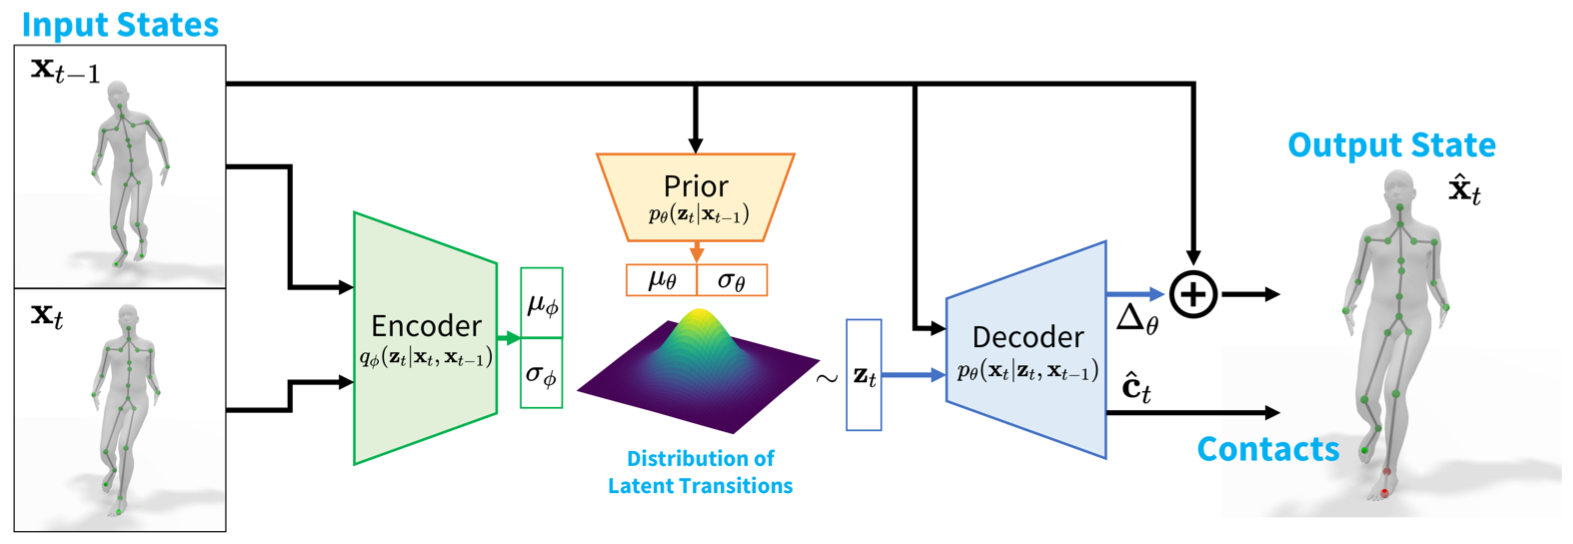
\includegraphics[width=1\textwidth]{Figures/humor/model/architecture.png}
    \caption{HuMoR C-VAE Architecture}
    \label{fig:humor_architecture}
\end{figure}


\TODO{Describe the model in more detail, include architecture diagrams etc., describe the rollout and the various stages of the model}

\section{HuMoR Investigation}
\label{sec:humor_investigation}

\subsection{Method}
Our investigation began with a largely qualitative evaluation of the HuMoR model which had two main aims.  First was to stress test the system, to see where it failed, where it succeeded, and if the mentioned benefits in the HuMoR paper \cite{humor} were as described.  The second was to evaluate the model with the defects of the current automated mocap system (described in \chpref{chpt:introduction}) in mind to see if it could complement its functionality, notably if it could improve upon occluded motion, joints flipping and confident but false predictions.

To achieve this goal, a selection of videos were taken containing a variety of motions; fast, slow, abnormal, and with occlusions. The HuMoR system was run on these videos and the results were investigated. The TestOps is performed in 3 stages as described in \secref{sec:humor_test_ops}, where only the 3rd makes use of the HuMoR motion model, we can therefore compare the Stage 2 results to the Stage 3 results to see where the model provided an improvement over a more classical optimisation method.

\subsection{Advantages of HuMoR}
We see a number of situations in which the model shows a clear improvement over stage 2 where the HuMoR model is not used.

In an occluded situation where the 2d pose predictions don't have any information on the legs, the model manages to produce a realistic sitting motion, as shown in \figref{fig:humor_sitting}.

\begin{figure}[!ht]
    \centering
    \subfloat[OpenPose]{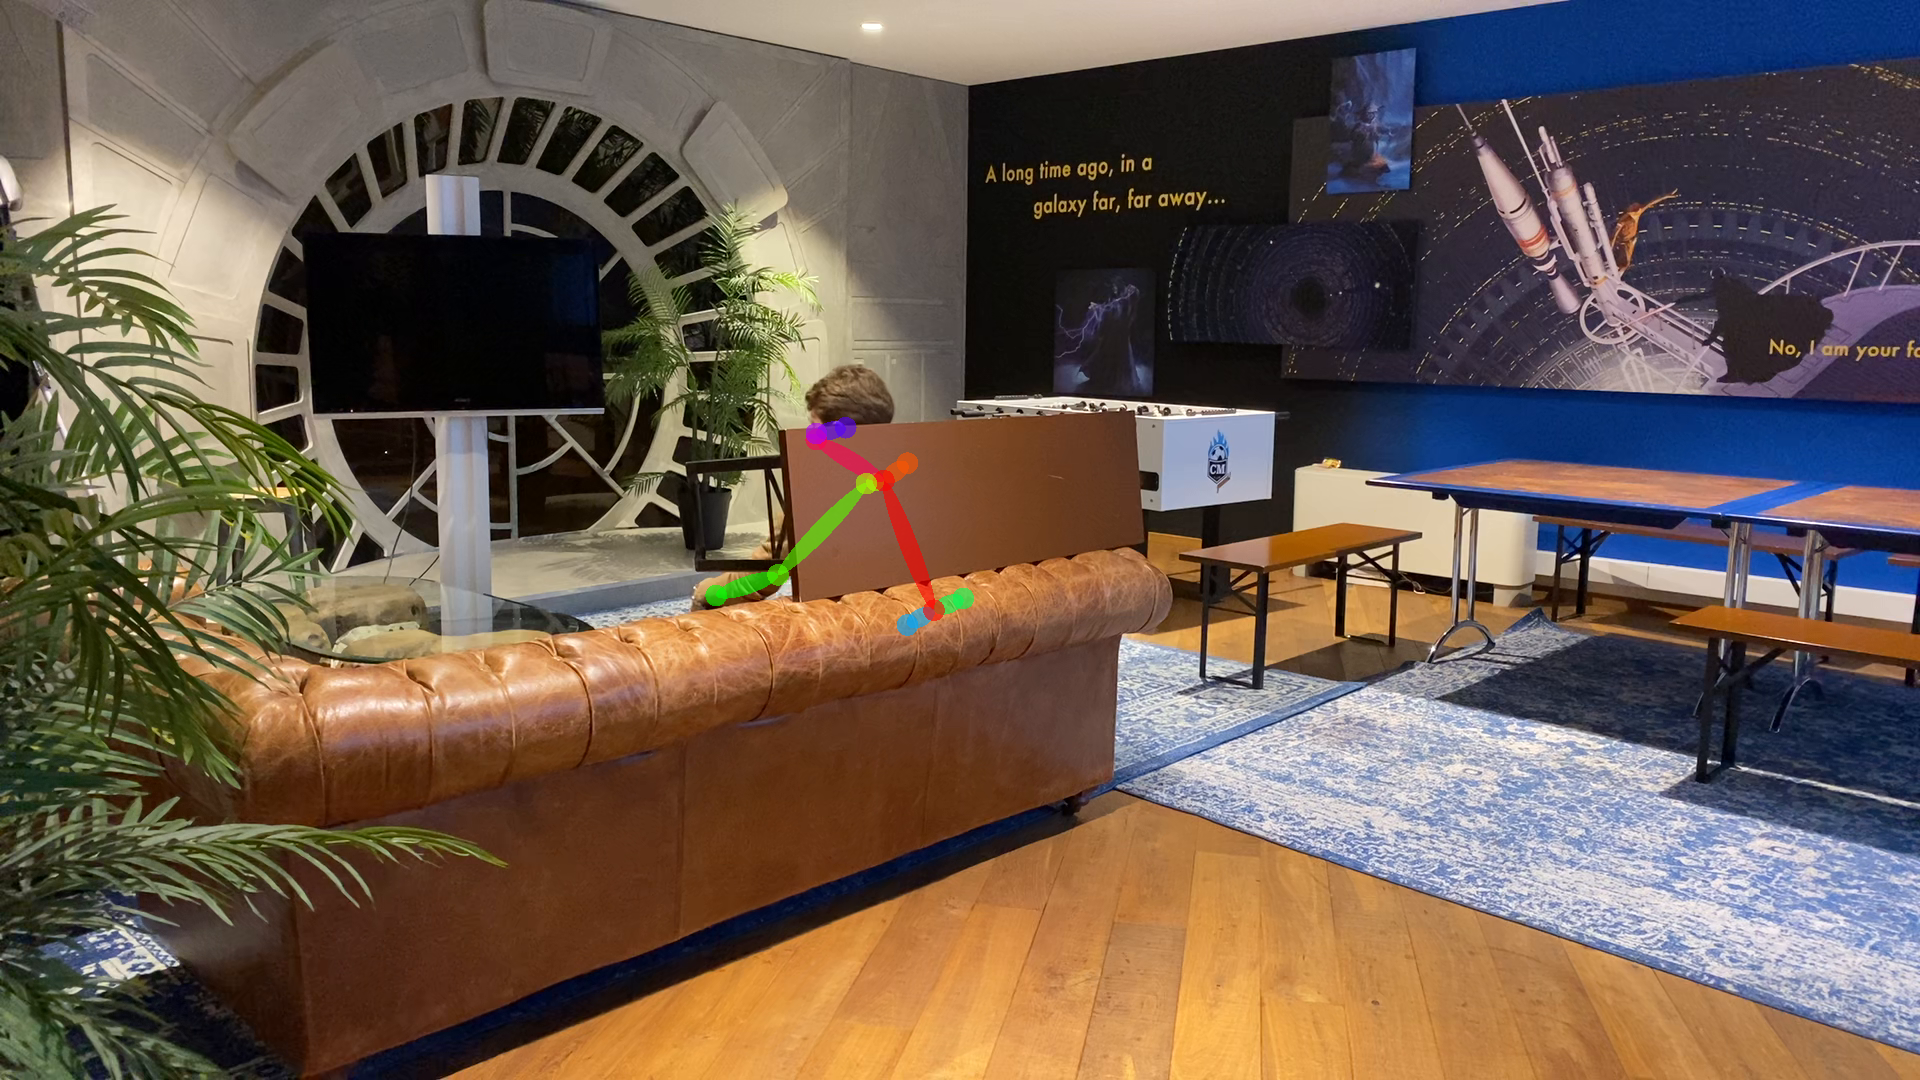
\includegraphics[width=0.3\textwidth]{Figures/humor/qualitative/good/sitting/openPose.png}} 
    \hfil
    \subfloat[Stage 2]{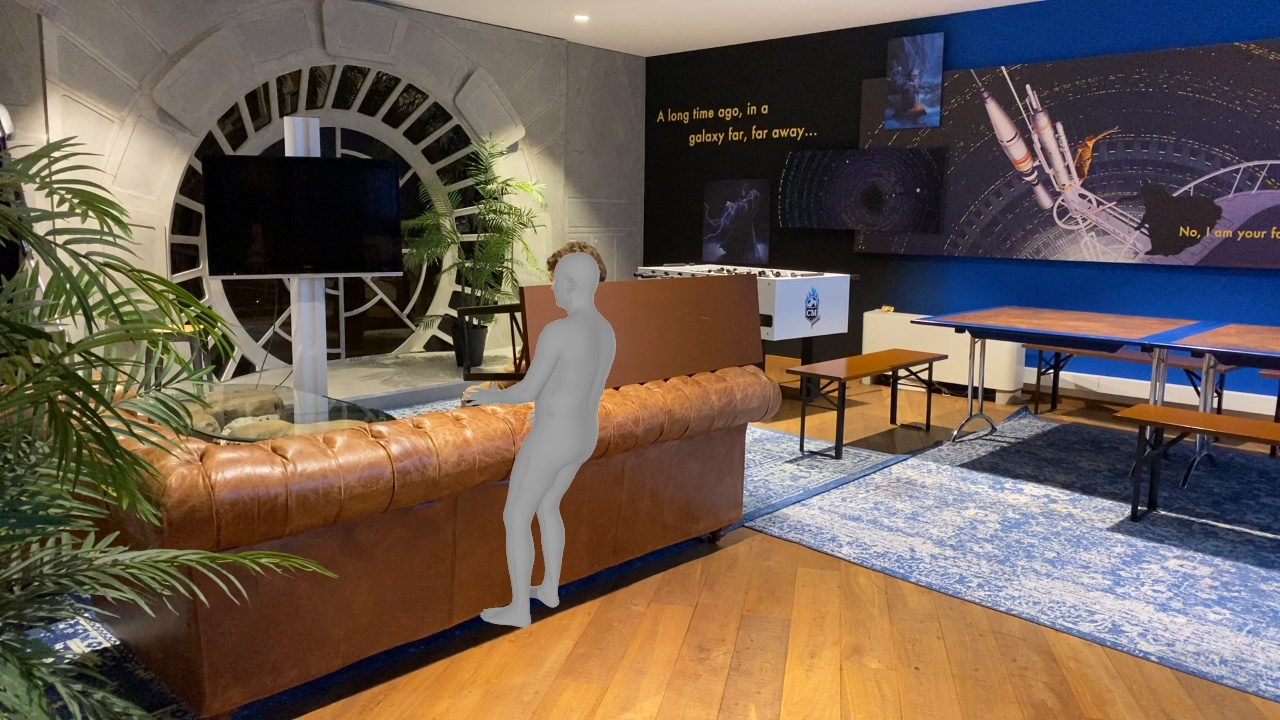
\includegraphics[width=0.3\textwidth]{Figures/humor/qualitative/good/sitting/stage2.jpg}} 
    \hfil
    \subfloat[Stage 3]{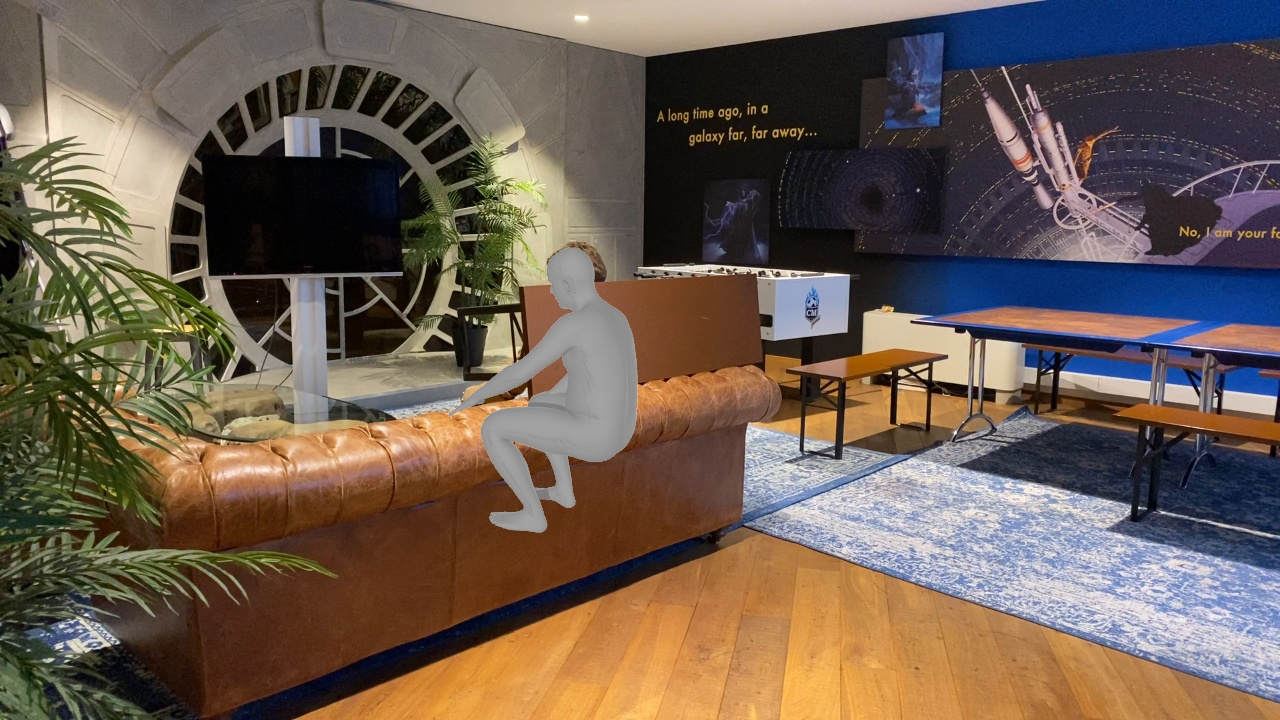
\includegraphics[width=0.3\textwidth]{Figures/humor/qualitative/good/sitting/stage3.jpg}}
    \caption{HuMoR achieving occluded sitting}
    \label{fig:humor_sitting}
\end{figure}

We also note that in many of the less complicated videos HuMoR produces clean motion and deals with many movements without obvious issues. It therefore doesn't seem to regress the easy situations but can improve the more difficult situations, notably occlusions.


\subsection{Drawbacks of HuMoR}

\subsubsection{Occluded walking}
We noted that while HuMoR manages to sit when occluded, it often fails to walk. This seems to be due to the fact that OpenPose \cite{openPose} often predicts both legs on the frames just before the occlusions where only one leg is actually un-occluded, as can be seen in \figref{fig:humor_bad_occluded_walking}. This results in a sequence of poses where the frames before an occlusion indicate that the person is no longer walking, hence making it significantly more difficult for HuMoR to begin walking again during the occlusion. This issue is thus largely due to a dependence on OpenPose and thus on an inheritance of OpenPoses' failure points.

\begin{figure}[!ht]
    \centering
    \subfloat[OpenPose]{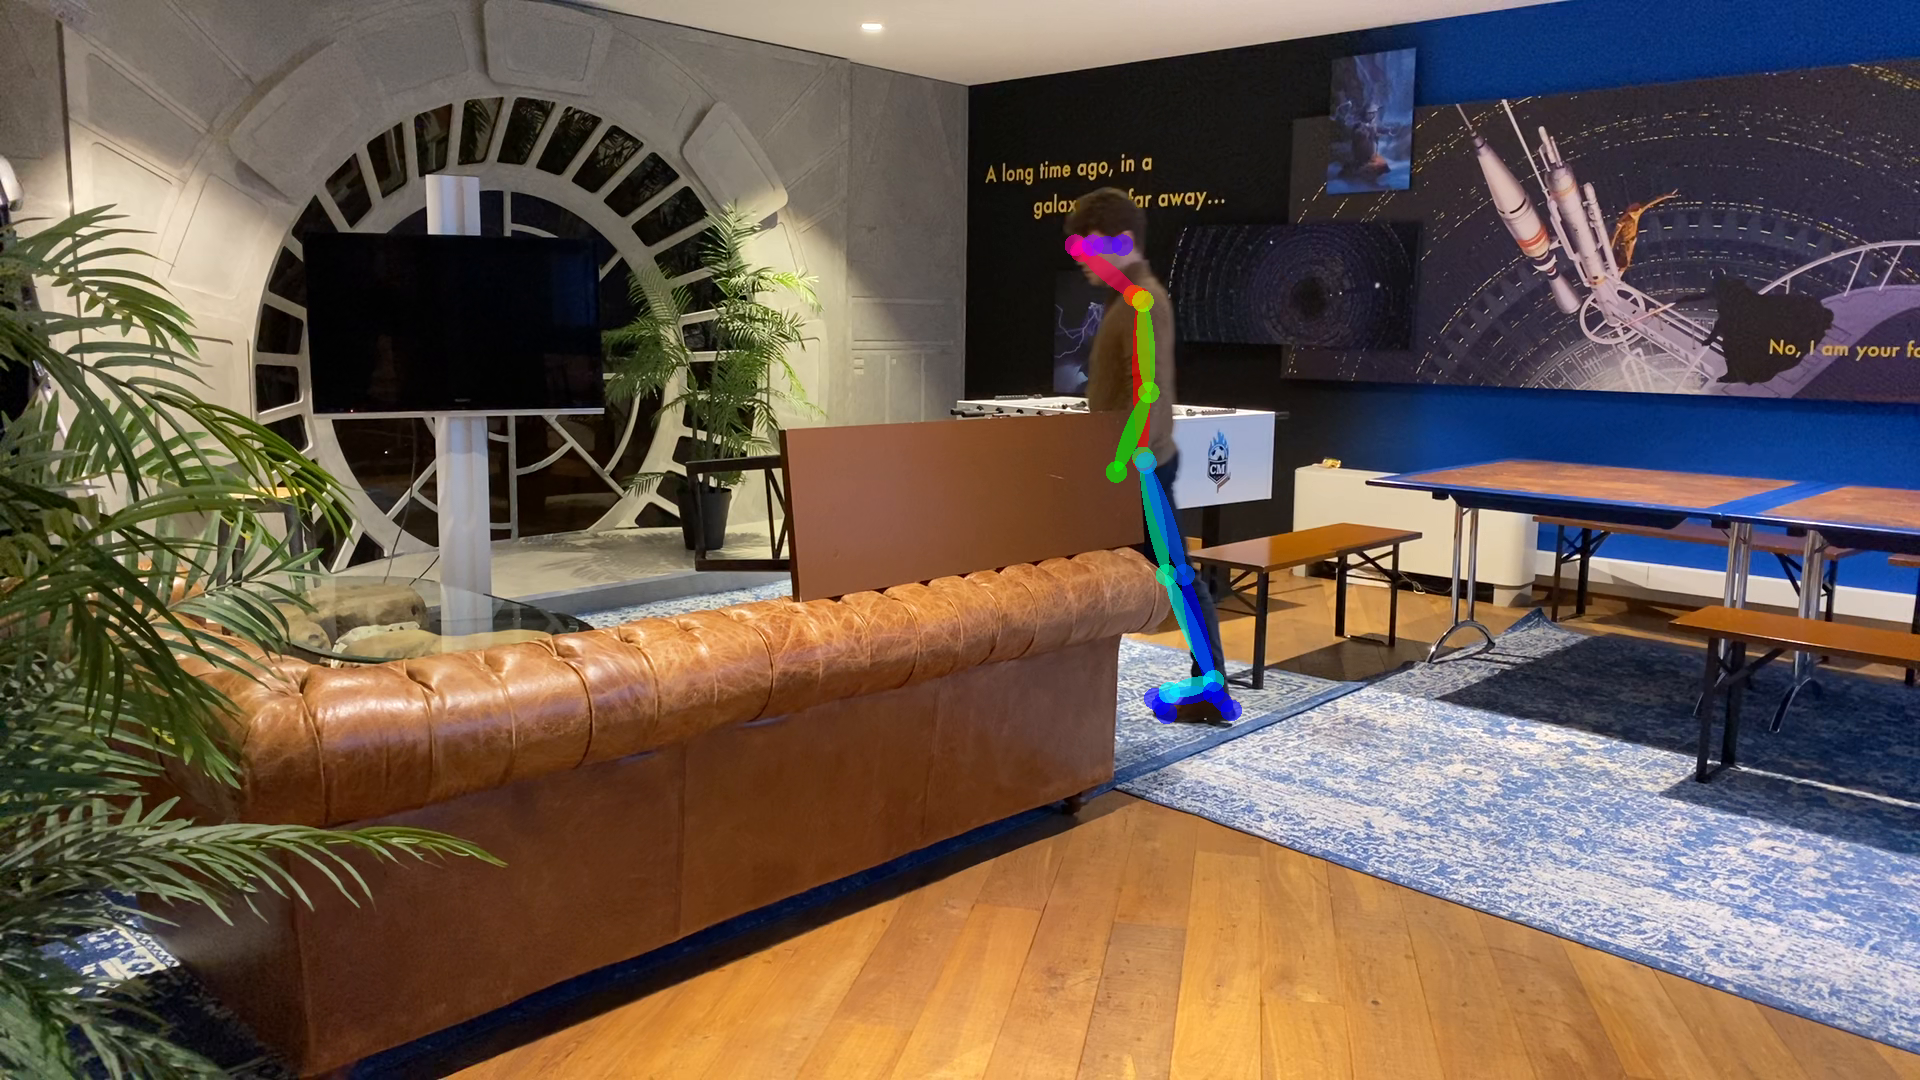
\includegraphics[width=0.2\textwidth]{Figures/humor/qualitative/bad/occluded_walking_failed/openPose.png}} 
    \hfil
    \subfloat[Stage 2]{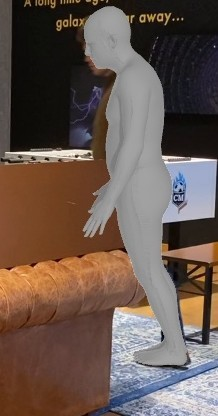
\includegraphics[width=0.2\textwidth]{Figures/humor/qualitative/bad/occluded_walking_failed/stage2.jpg}} 
    \hfil
    \subfloat[Stage 3]{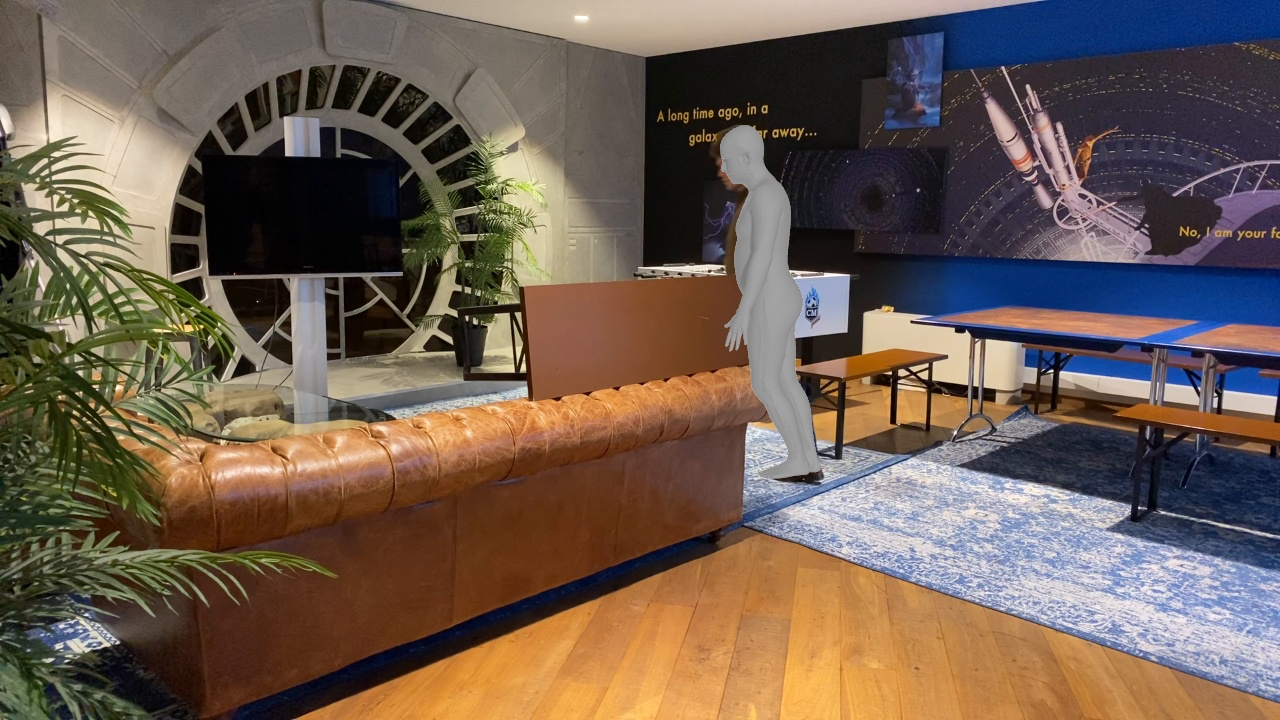
\includegraphics[width=0.2\textwidth]{Figures/humor/qualitative/bad/occluded_walking_failed/stage3.jpg}}
    \caption{Occluded walking failure point, 2 legs predicted instead of 1}
    \label{fig:humor_bad_occluded_walking}
\end{figure}

\subsubsection{Axis-angle representation}
We also found that the choice of axis angle representation for various rotations led to the emergence of commonly known issues that arise from the discontinuities present in the representation \cite{aa_6d_angles}. The shortest path between certain angles in axis angle space enforced by the smoothness regularizer can lead to a 360-degree rotation, as seen in \figref{fig:humor_bad_aa}, among other issues.

\begin{figure}[!ht]
    \centering
    \subfloat[Raw frames]{
        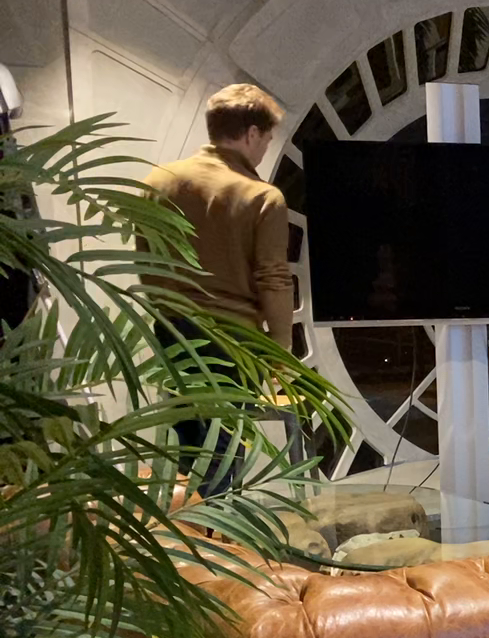
\includegraphics[width=0.2\textwidth]{Figures/humor/qualitative/bad/aa_issue/000329.png}
        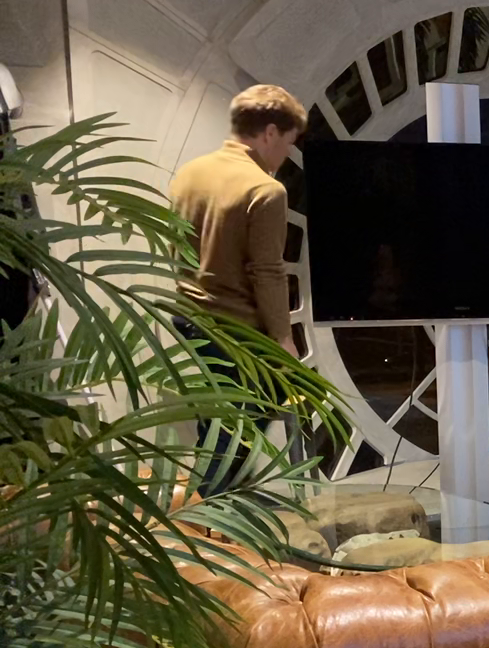
\includegraphics[width=0.2\textwidth]{Figures/humor/qualitative/bad/aa_issue/000335.png}
        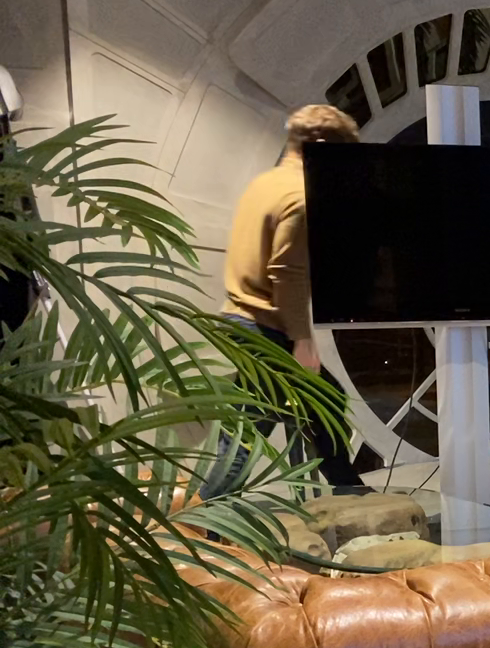
\includegraphics[width=0.2\textwidth]{Figures/humor/qualitative/bad/aa_issue/000343.png}
    } 
    \hfil
    \subfloat[OpenPose]{
        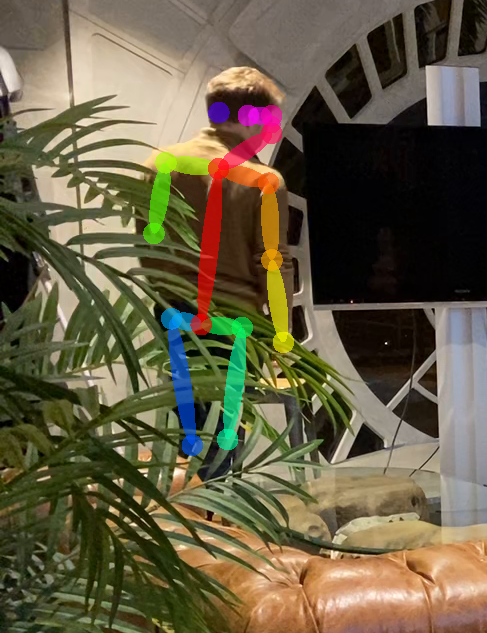
\includegraphics[width=0.2\textwidth]{Figures/humor/qualitative/bad/aa_issue/000329_rendered.png}
        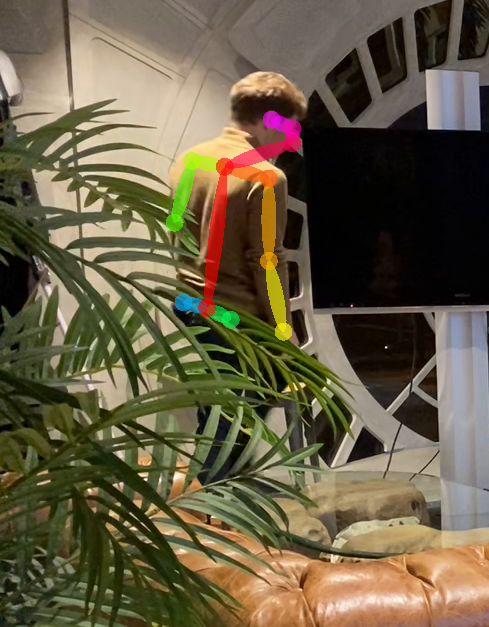
\includegraphics[width=0.2\textwidth]{Figures/humor/qualitative/bad/aa_issue/000335_rendered.png}
        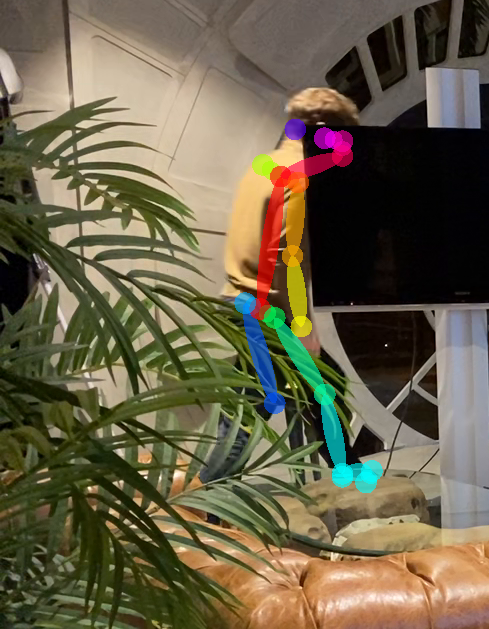
\includegraphics[width=0.2\textwidth]{Figures/humor/qualitative/bad/aa_issue/000343_rendered.png}
    }
    \hfil
    \subfloat[HuMoR, note the full rotation to the left]{
        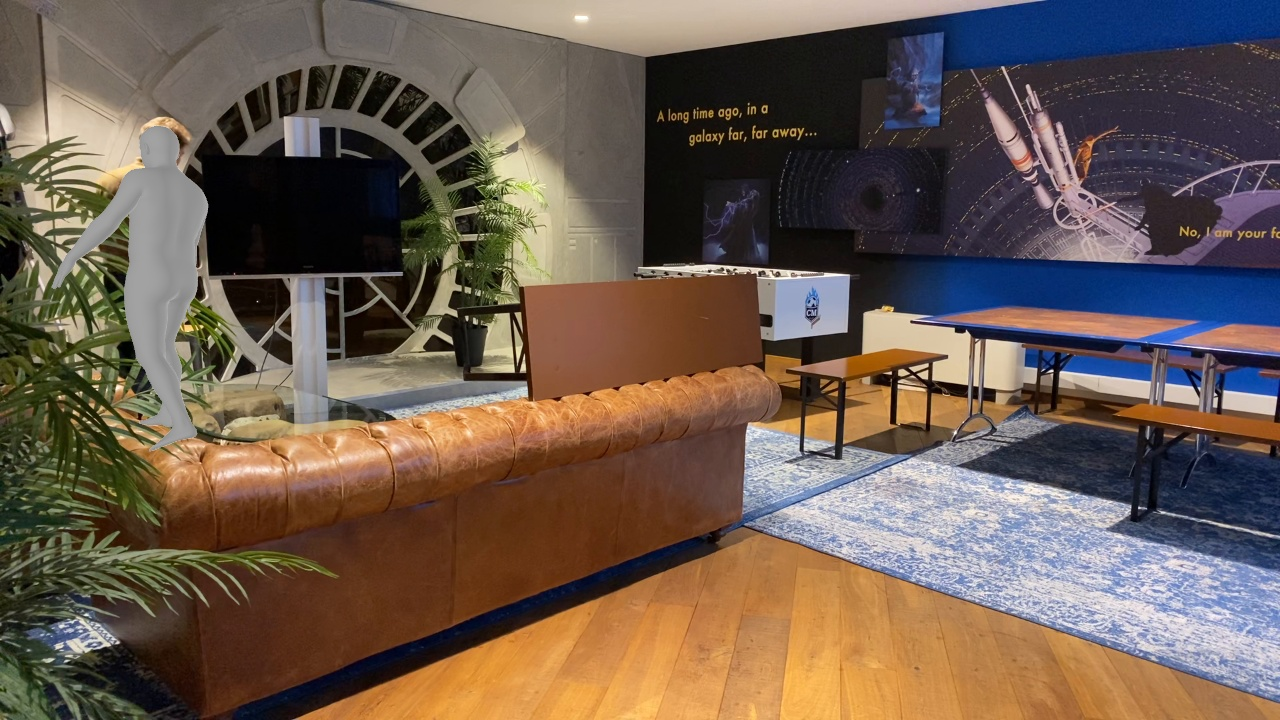
\includegraphics[width=0.2\textwidth]{Figures/humor/qualitative/bad/aa_issue/frame_00000329.jpg}
        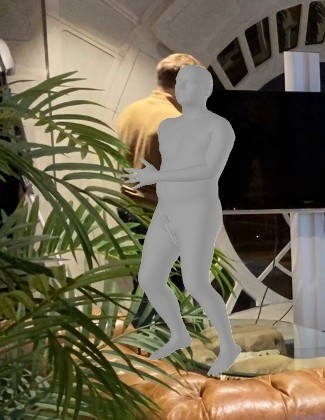
\includegraphics[width=0.2\textwidth]{Figures/humor/qualitative/bad/aa_issue/frame_00000335.jpg}
        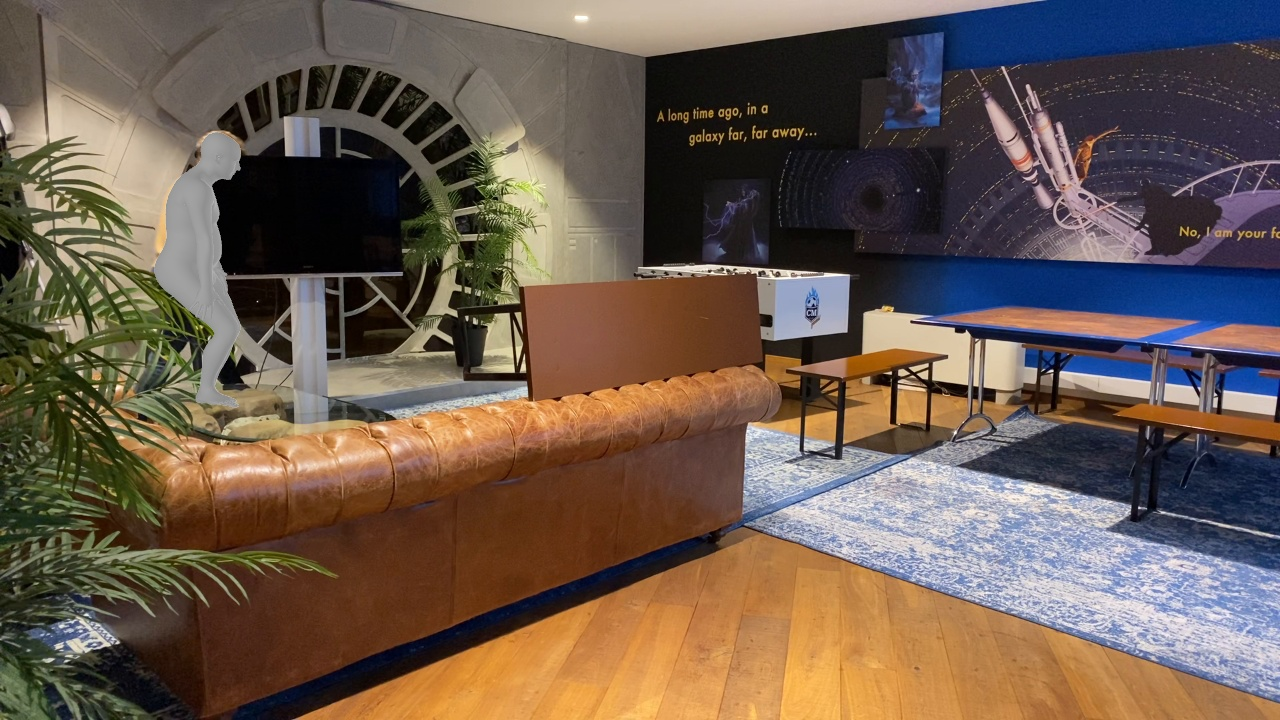
\includegraphics[width=0.2\textwidth]{Figures/humor/qualitative/bad/aa_issue/frame_00000343.jpg}
    }
    \caption{Axis angle issue: dubious rotations}
    \label{fig:humor_bad_aa}
\end{figure}

\subsubsection{Over-smoothed motion}
Next, we saw overly smoothed motion for certain clips, most notably for particularly stylised motions such as dancing.  We also found that if there is a single frame without OpenPose predictions then from that frame onwards the TestOps fails. 

\subsubsection{Autoregressive nature}
We found that the TestOps system would occasionally get itself into a tangle, as seen in \figref{fig:humor_bad_mess}, we assume due to the autoregressive nature resulting in a potentially catastrophic cumulation of errors and found this happened most notably for a sequence containing someone rolling on the floor. It is interesting to note that these sorts of motions were not often, if ever, present in the training data, and so it is likely that the model can fail catastrophically in many more situations, provided that they are sufficiently different from the training data.

\begin{figure}[!ht]
    \centering
    \subfloat[OpenPose]{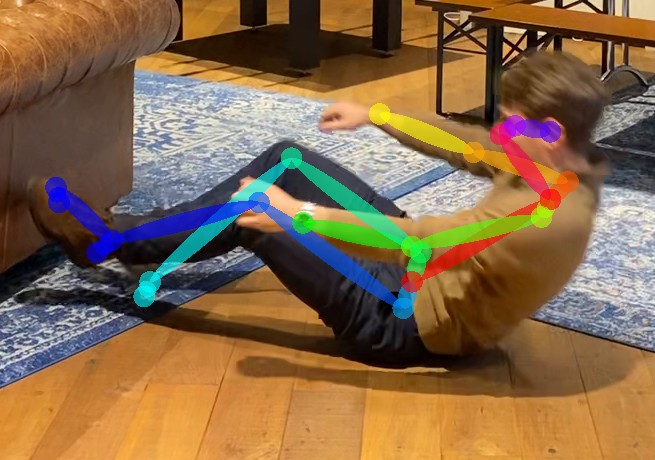
\includegraphics[width=0.3\textwidth]{Figures/humor/qualitative/bad/unrecoverable/openPose.png}} 
    \hfil
    \subfloat[Stage 2]{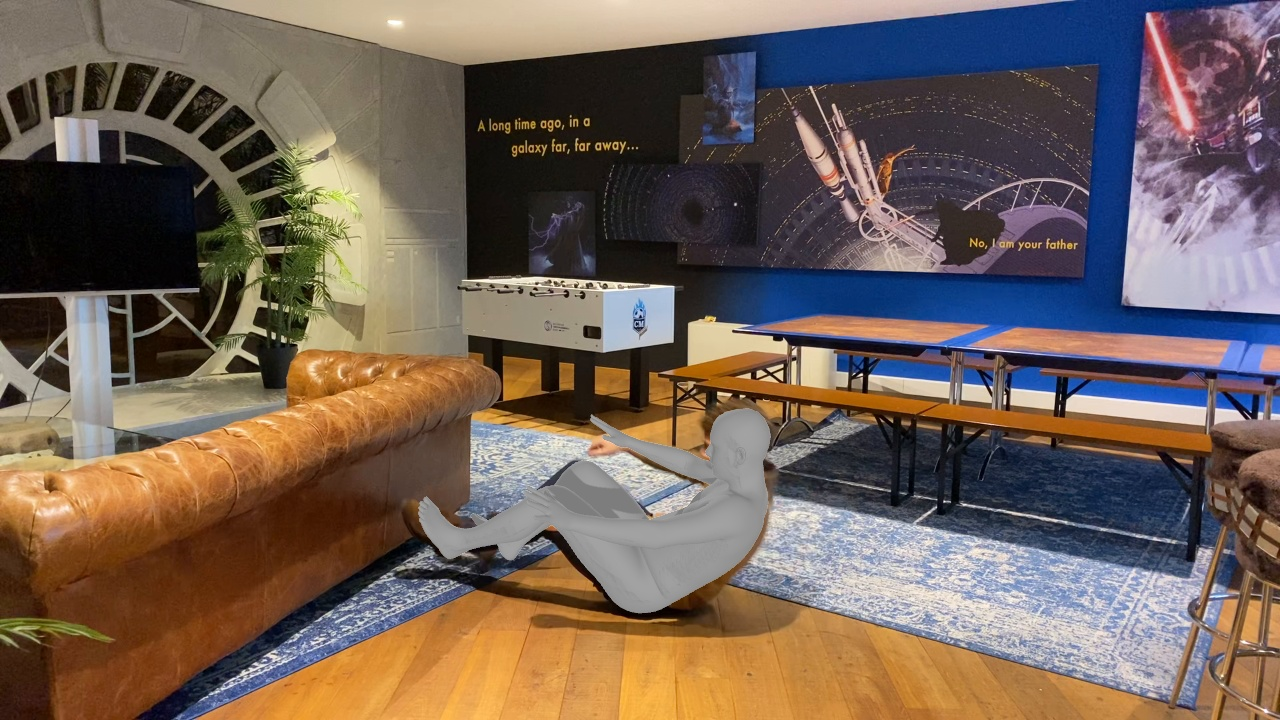
\includegraphics[width=0.3\textwidth]{Figures/humor/qualitative/bad/unrecoverable/stage2.jpg}} 
    \hfil
    \subfloat[Stage 3]{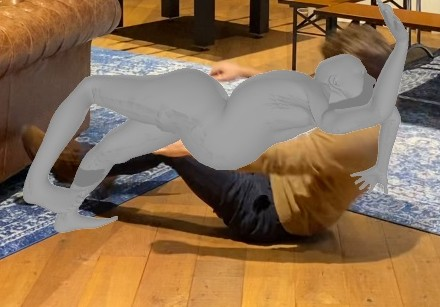
\includegraphics[width=0.3\textwidth]{Figures/humor/qualitative/bad/unrecoverable/stage3.jpg}}
    \caption{HuMoR in a tangle}
    \label{fig:humor_bad_mess}
\end{figure}

Another issue due to the autoregressive nature was the computational burden and high memory usage. The system splits a full video into multiple overlapping subsequences as it is not computationally practical to roll out for the entire sequence. The overlapping sections then have an additional loss applied to them to ensure consistency between the subsequences. While reasonably effective, this demonstrates the heavy computation burden of a long-range autoregression and we find that the shorter the subsequences, the more discontinuities in the optimised motion.

Finally, and most importantly, we found that the TestOps was extremely slow. It took around 20mins per 2s clip, and we could batch at most four 2s clips together, totaling 20mins per 8s on an Nvidia GeoForce 1080ti with 11Gbs memory.

\subsection{Profiling}
To further investigate this speed issue, we profiled the code, as can be seen in \figref{fig:humor_profiling}. We found that the program spent 90\% of its time in the Stage 3 optimiser closure, 56\% of its time performing the backward step and 32\% of its time in the rollout function. Hence it was clear that the speed issue was due to the slow act of rolling out in stage 3 and the large computation necessary to perform the backward step on the enormous computation graph resulting from the rollout.

\begin{figure}[!ht]
    \centering
    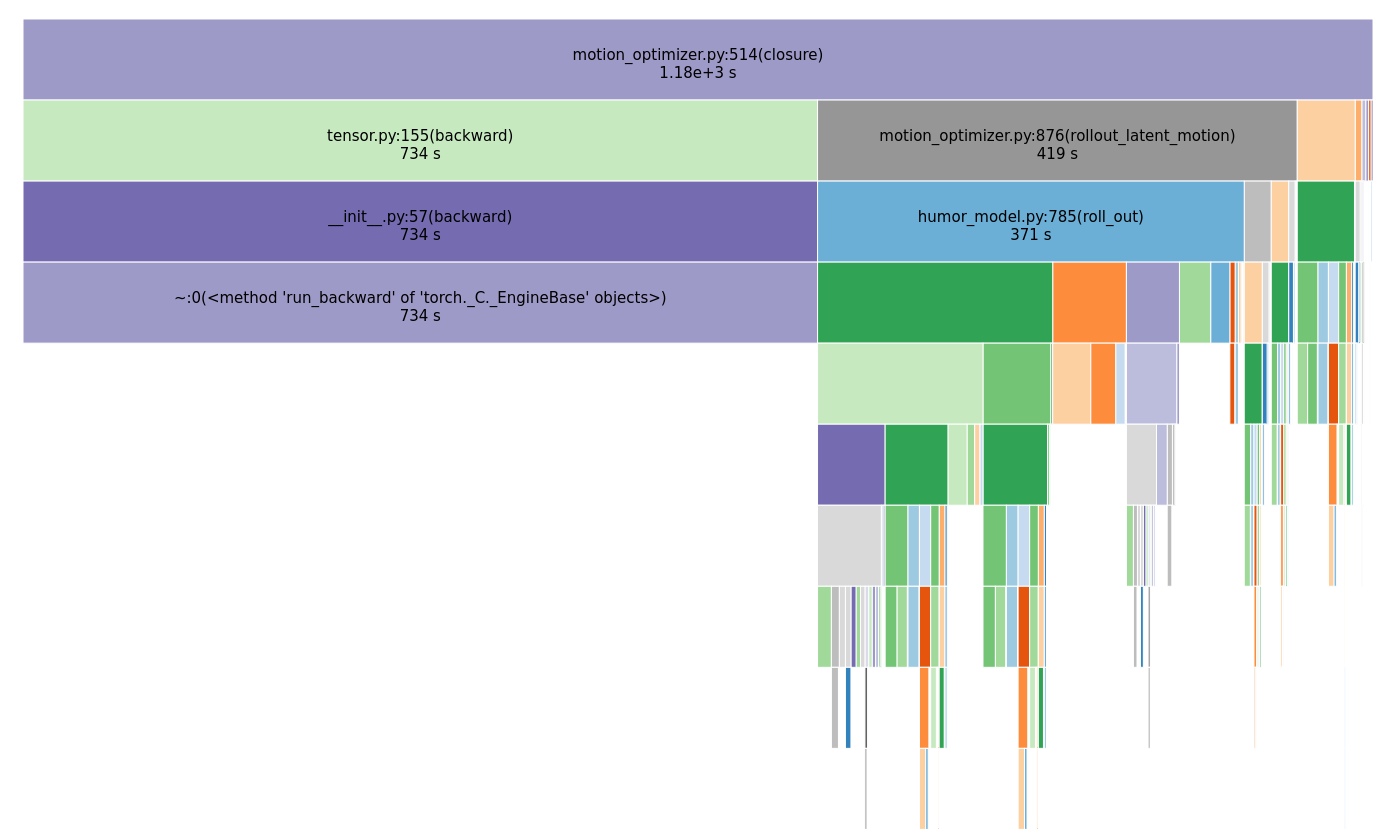
\includegraphics[width=1\textwidth]{Figures/humor/profiling/profiling.png}
    \caption{TestOps profiling}
    \label{fig:humor_profiling}
\end{figure}

\subsection{Investigation Conclusion}
Through this investigation, we found that HuMoR demonstrates a number of positive properties. The model handles occluded sitting motions well and often creates clean and plausible motion. It does however also exhibit numerous issues. The choice of axis angle representation, the dependence on OpenPose, and the smoothed motion all had a good chance of being fixed with different optimiser design choices.  The glaring issue however was the unresonable amount of time the system took, rendering it unusable for our desired goal of having a close to real-time motion capture system. The next step was therefore to speed up the method, and to do so we needed to focus primarily on improving/removing the rollout of the third stage of the optimiser. In the next section, an attempt to do just this is presented.
\section{Improving HuMoR TestOps}
\label{sec:humor_improvement}

This section presents the attempt that was made at modify the TestOps of the HuMoR paper \cite{humor} in such a way that we attain comparable results but in a significantly shorter timespan.

\TODO{See if I have introduced the terms properly (decoded sequence, $x$'s, $x'$'s, etc.)}

\subsection{Speeding up the TestOps}

Realising that the main speed limitations are due to the concept of rollout over the entire sequence, we decided to break this long range dependence. Through short overlapping rollouts, it is possible to acheive more parrallelisation and smaller computation graphs, and our intuition suggests that the need for such a large context window is not necessary, that only a small number of autoregressed frames are needed to be able to propagate information sensibly and to get meaningful gradients. Anecdotaly, it would seem intuitive that if a video contains sitting, then walking, then sitting again, the second act of sitting would not depend in on the early act of sitting, hence rolling out over the whole sequence seems unnecessary.

The HuMoR TestOps rollout is presented graphically in \figref{fig:humor_rollout_graph}. $x$ is the state, and $z$ are the latent variables, the optimised variabels are highlighted in pink, and the losses are coloured, gray x's indicate they are calculated during the optimisation from the optimised variables. As can be seen, first all the states are autoregressed from the initial state and the latent variables, and then the losses are applied. This can be seen to result in very long range dependencies in the computation graph, thus making the gradients time consuming to calculate. 

\begin{figure}[!ht]
    \centering
    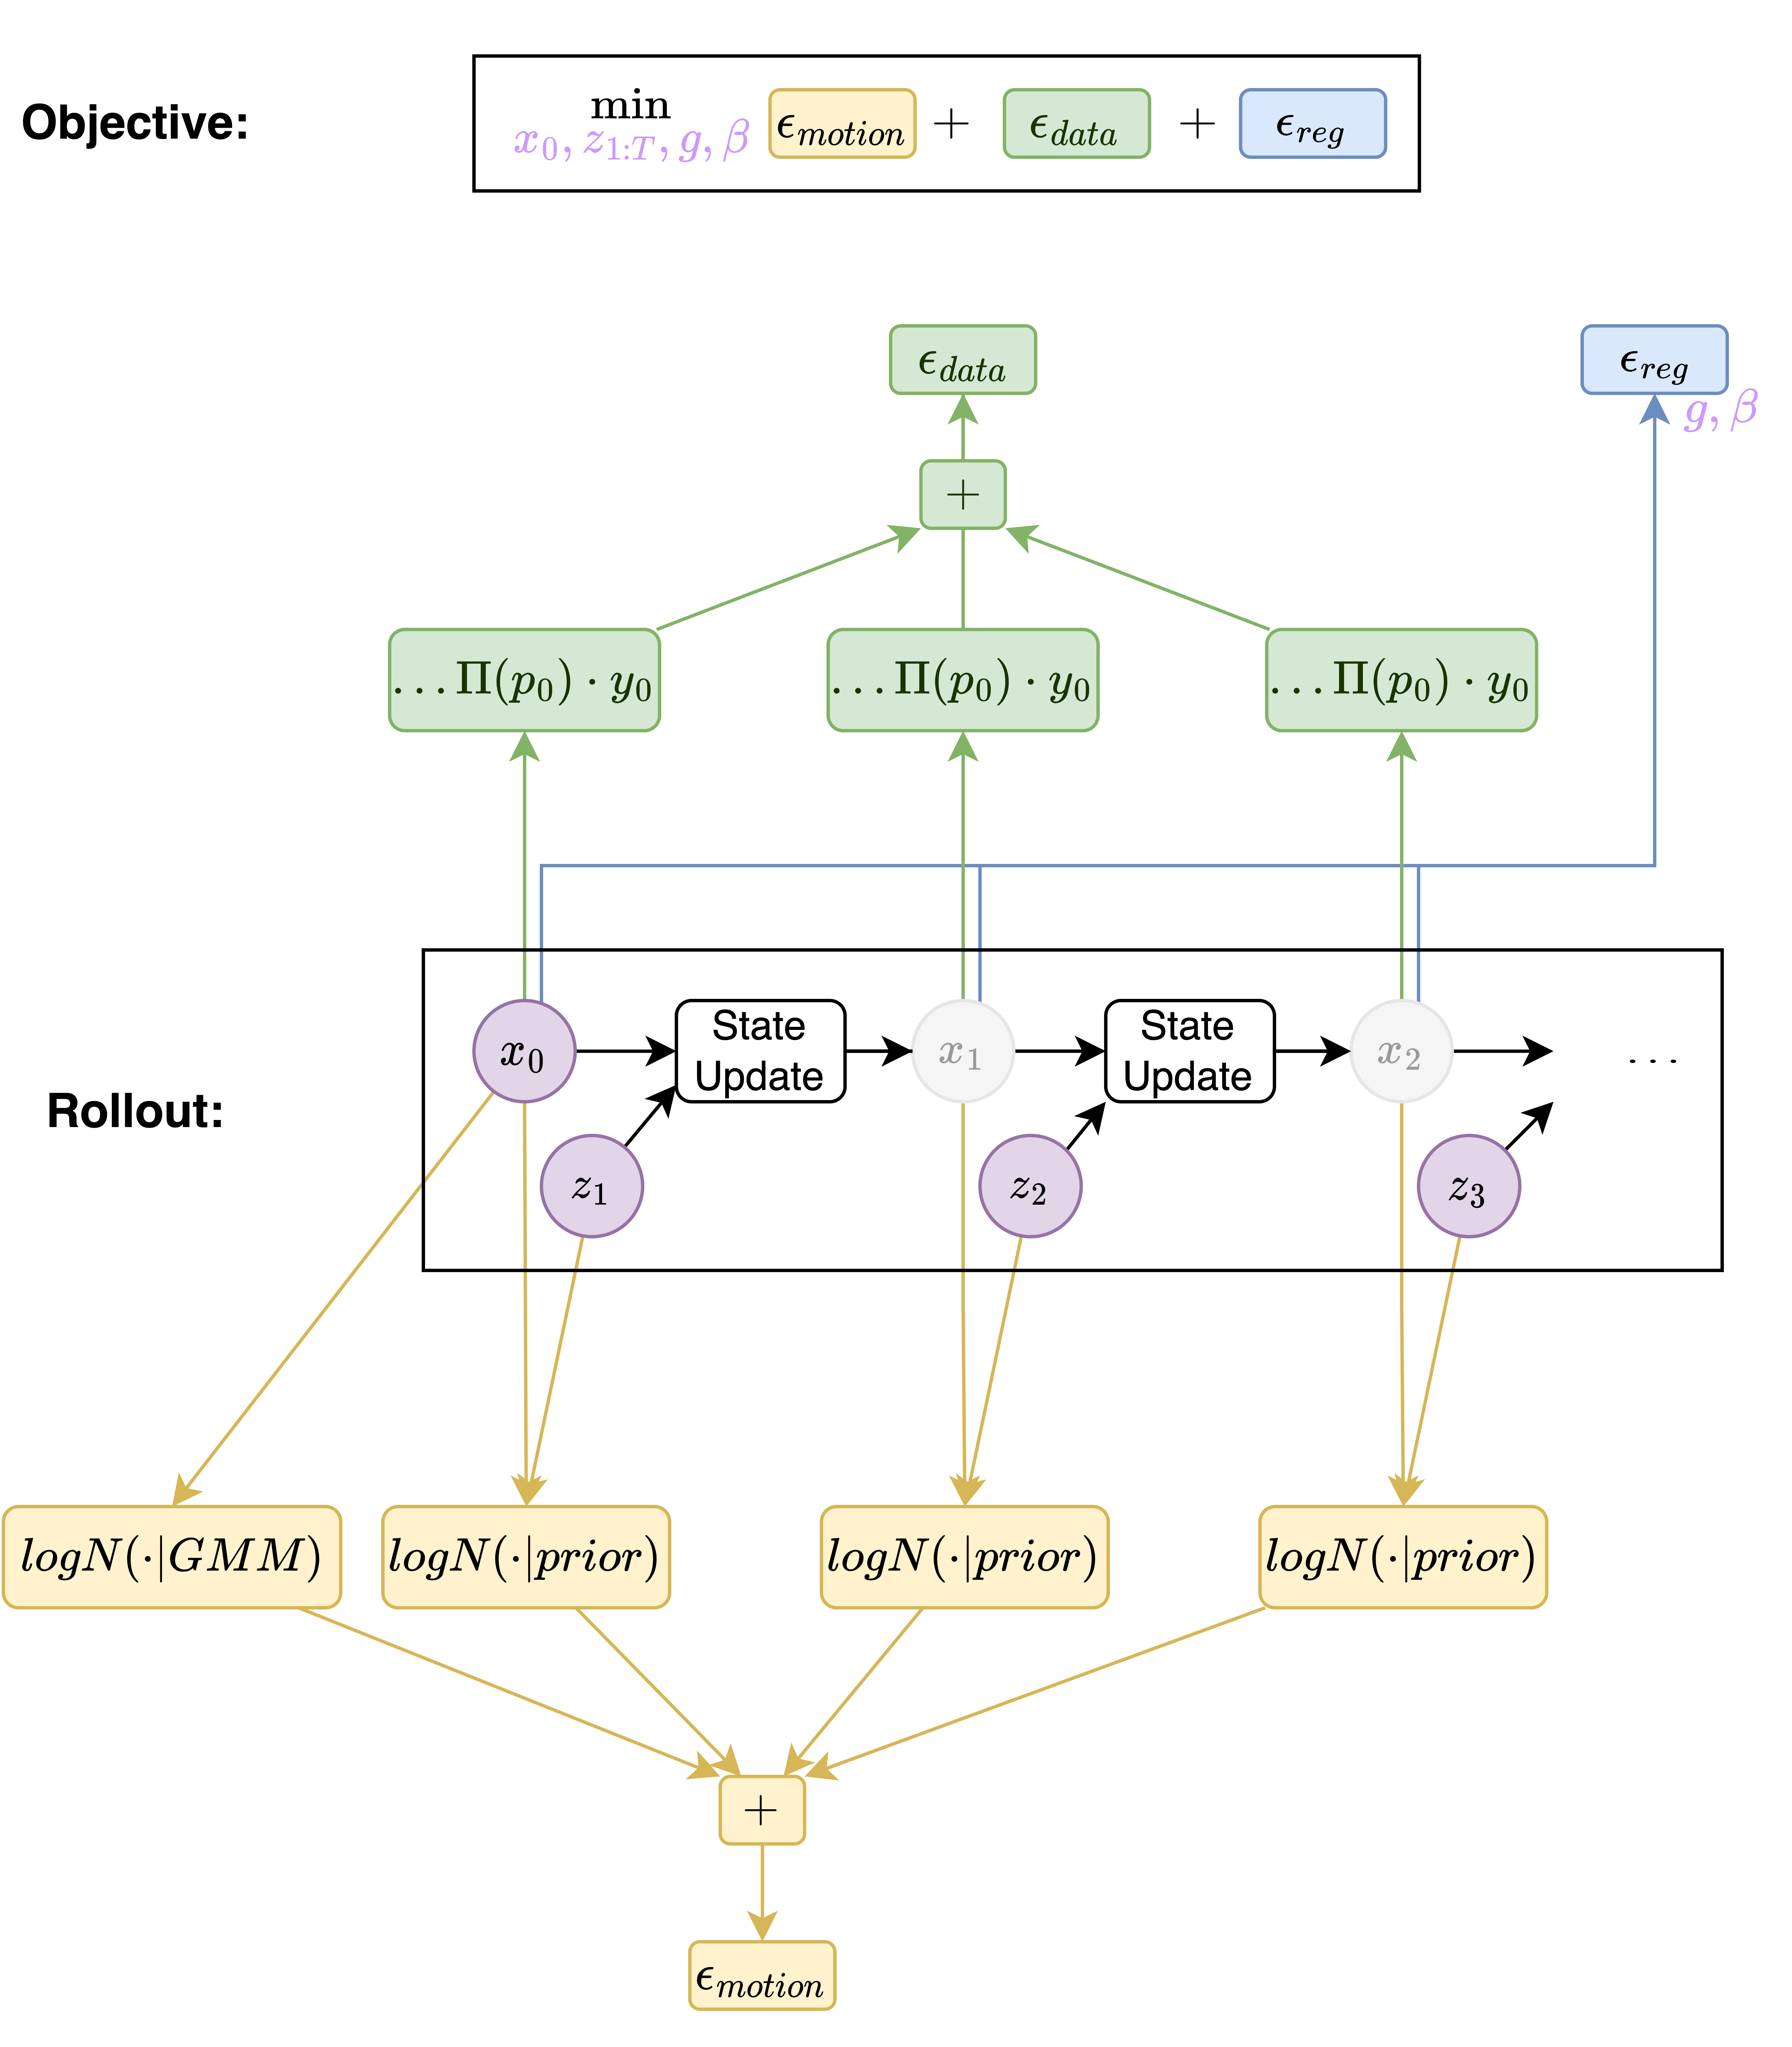
\includegraphics[width=1\textwidth]{Figures/humor/improvement/computation_graph_humor.png}
    \caption{TestOps Computation Graph}
    \label{fig:humor_rollout_graph}
\end{figure}

\TODO{Update \figref{fig:dimm_rollout_graph} and remove the 'NEW' norm, labels on green loss, and potentially red loss?}

The most obvious way to break this autogregression is to maintain and optimise a separate sequence of $x$'s, updating this seperate sequence with reference to the $x'$'s decoded from the latent variables as in \figref{fig:dimm_rollout_graph}. We can take into account the decoded $x'$'s in several manners:
\begin{itemize}
    \item Copy over
    \begin{itemize}
        \item Directly replace the optimised sequence of $x$'s with the decoded $x'$'s.
    \end{itemize}
    \item Blend
    \begin{itemize}
        \item Perform a weighted addition of the optimised $x$'s and decoded $x'$'s.
    \end{itemize}
    \item Loss term
    \begin{itemize}
        \item Add a loss term on the difference between the optimised $x$'s and decoded $x'$'s. 
    \end{itemize}
\end{itemize}

All decoding steps can now be performed in parrallel, rather than sequentially, which greatly reduces the computation time. 

\begin{figure}[!ht]
    \centering
    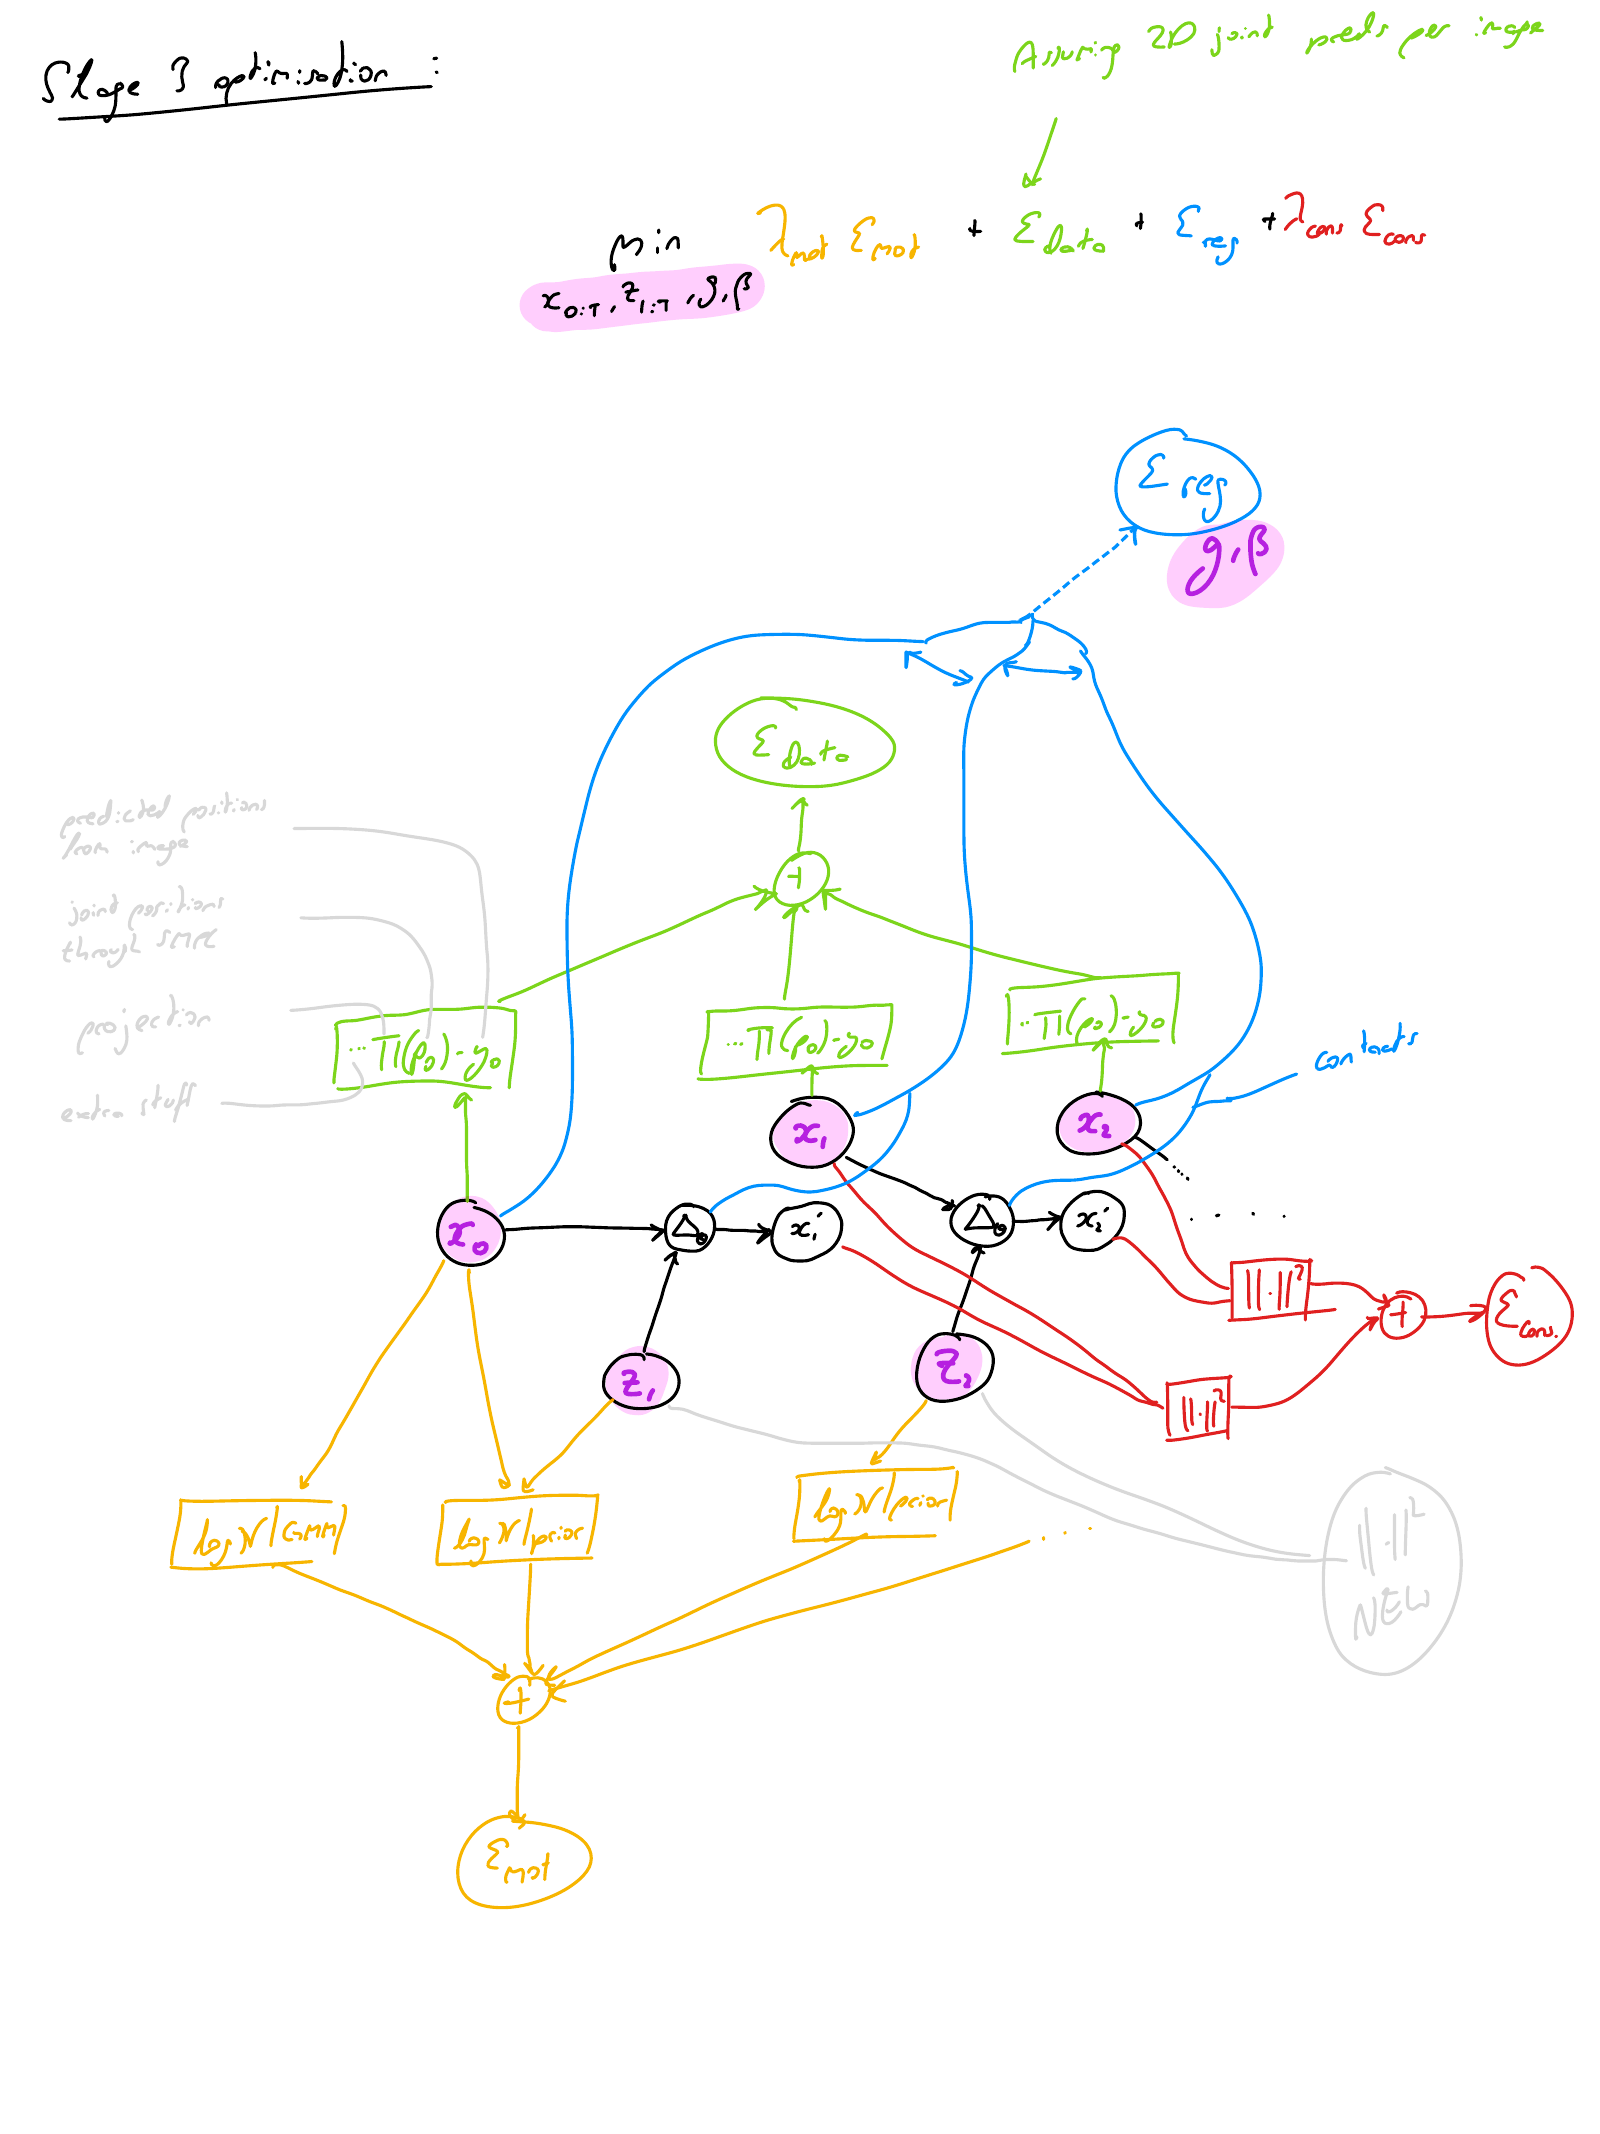
\includegraphics[width=1\textwidth]{Figures/humor/improvement/computation_graph_dimm.png}
    \caption{Decoupled Computation Graph}
    \label{fig:dimm_rollout_graph}
\end{figure}

This new method also allows us to experiment with different amounts of rollout. We can once again decode the decoded sequence of $x'$'s to get $x''$, and so on and so forth. These extra sequences are all decoded with the same latent variables thus the updates to the latent variables will take into account the losses on all the decoded sequences. Graphically this can be seen in \figref{fig:dimm_decoded_sequences}, where each next line .
\TODO{describe the figure better}

\begin{figure}[!ht]
    \centering
    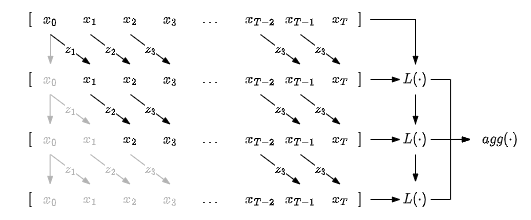
\includegraphics[width=1\textwidth]{Figures/humor/improvement/Rollout_overlap.png}
    \caption{Decoded sequences}
    \label{fig:dimm_decoded_sequences}
\end{figure}

The information contained in each $x$ can flow forwards through the short range rollouts, and over the iterations of the optimiser. Note however that the information flow will be slower than the HuMoR TestOps, as in the TestOps all subsequent $x$'s are regressed from the initial $x_0$.
In the HuMoR TestOps information can flow backwards from any future frame's $x$ in one update through the gradients, as all $x$'s are linked in the computation graph through the auto-regression (though our intuition suggests that the information does not actually need to flow so far, as previously discussed). In the new method however, the information flow will be much more limited, as the rollouts will be significantly shorter, though again the information should flow through the iterations fo the optimiser.

\subsection{Implementation notes}

A number of issues were encountered during the implementation that are worth mentioning. After implementing the new method, attempts were made to get the optimiser to produce sensible results. The general approach was to use a small number of losses, so as to get a better intuition of each loss, with the goal of better understanding how to balance the losses in the optimiser, but some errors in individual losses were encountered.

Firstly, as expected, the Axis-Angle representation became a problem. When running through functions to convert to root-local reference frame for the HuMoR model for decoding (as it operates on said reference frame), and then back to world reference frame for the opftimiser, the Axis-Angle vector flipped direction. Though the flipped vector still represented the same rotation, the angle representations of the same angle in the optimised sequence of $x$'s and the decoded sequence of $x'$'s were different, hence encorporating the information from decoded sequence cause the angle to move somewhere between the two flipped values which was no longer a sensible angle representation, thus resulting in root flips and other strange effects.

Secondly, an issue due to the SMPL model was found. When using a 2d reprojection loss (comparing the projected SMPL joints to the OpenPose 2d predictions) on a sequence where only the left arm and face had any OpenPose predictions, the legs were being moved by the optimiser. This was wrong as there were only losses on the arm and face joints, hence no gradients should flow to the legs. It was eventually found that the skinning weights of the SMPL model \cite{SMPL} contain spurious long range connections. 3\% of the LBS (linear blend skinning) weights in the SMPL model are non-zero but less than $1e-2$, which seems rather too low to have any meaningful effect on the skinning, but which allows for spurious gradients to flow. \\
For the comparison to the OpenPose predictions the OpenPose skeleton must be obtained from the SMPL mesh. Certain joints are regressed, other are simply taken directly as vertices from the mesh, as in the case of the nose joint in the OpenPose skeleton which is taken to be vertex 332 \cite{SMPL_op_joints}. We noted that this vertex 332 is skinned $99.8\%$ by the 'head' joint, but also $0.2\%$ by the right hip, left knee and right knee. This issue was solved by pruning all weights below 1e-2. It is interesting to note that there are known spurious connections in the SMPL blend shapes \cite{STAR}, but that we have found no reference to spurious connections in the LBS weights.

\subsection{Experiments}

% c.f Current_experiments.md for more details
\TODO{explain why the initial rollout was bad, and the compounding of errors forward}
\TODO{maybe we should discuss more in the humor investagtion section about the bad initial rollout}
\TODO{Check everything is explicitely named, e.g have a graphic clearly naming the optimised x's and the decoded x's, and what the z's are}

To begin with, we looked into the initial $z$'s that were obtained from projecting the Stage 2 results through the HuMoR encoder. We found that in occluded situations these $z$'s encode a sitting motion without any optimisation as seen in \figref{fig:humor_stage_2_rollout_sitting}, that simply the projection leads them to encode the necessary occluded motion. However we note that when autoregressively rolled out over a longer sequence the results, in \figref{fig:humor_stage_2_rollout_deviation}, deviate largely from the initial sequence of $x$'s seen in \figref{fig:humor_stage_2}. This shows us that though the initial $z$'s encode some sensible motion locally, and can be used to accurately recover the next frame, when they are chained together small deviations from the $x$ motion accumulate to create an overall deviation. For example if the arm is moved slightly too much by a single $z$, then all the future frames will have the arm in slightly the wrong position, and multiple $z$'s are wrong in the same direction, then the arm will raise up. This deviating sequence is the initial starting rollout in the Stage 3 of the HuMoR TestOps in which the rollout is optimised, though it seems unfortunate to us that from a sensible sequence of $x$'s obtained from Stage 2 we get such a bad sequence through the autoreggresive rollout. We do however note that though while this starting point represents a sequence that deviates largely, the $z$'s might not need to move so far to avoid the accumulation effect. The intuition in our case was that we are starting from some sensible $x$'s and $z$'s, and therefore that it should be possible to refine the $x$'s by take into account the HuMoR model through the $z$'s whilst updating the $z$'s. 

\begin{figure}[!ht]
    \centering
    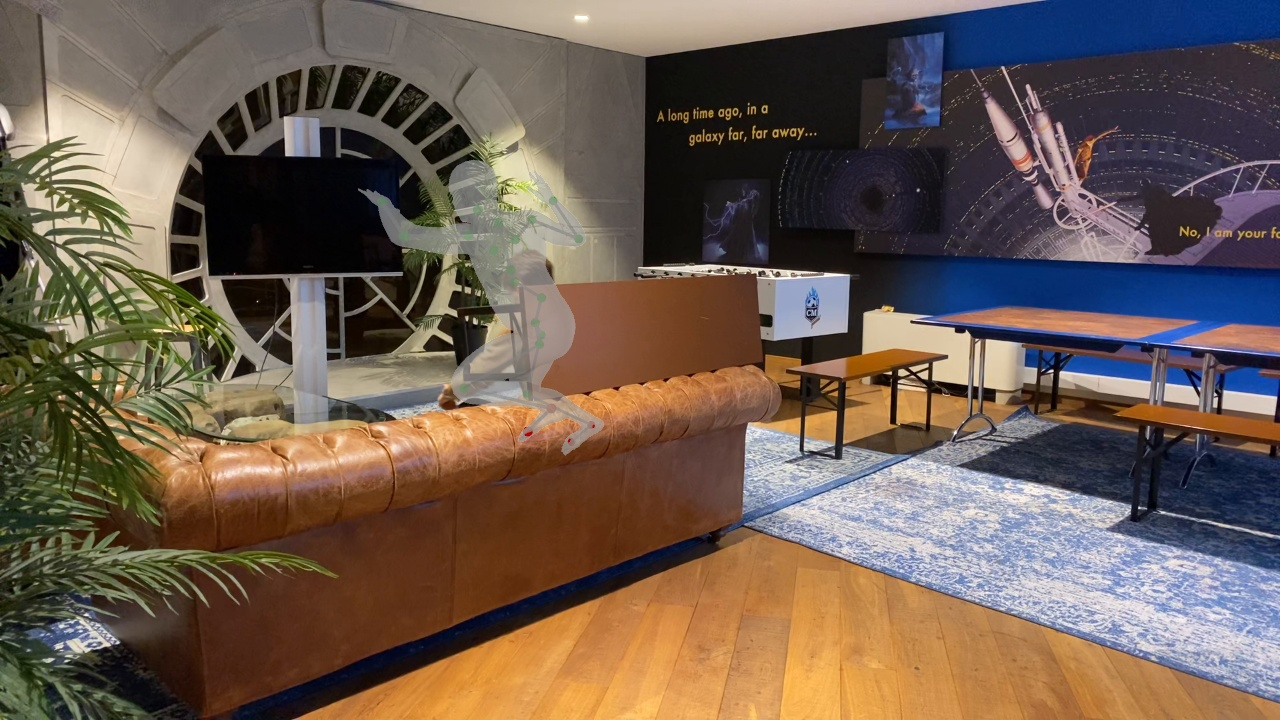
\includegraphics[width=1\textwidth]{Figures/humor/improvement/Rollout_stage_2/sitting_clip/rollout_sitting_example/frame_00000078.jpg}
    \caption{Stage 2 $z$'s encode a sitting motion}
    \label{fig:humor_stage_2_rollout_sitting}
\end{figure}


\begin{figure}[!ht]
    \centering
    \subfloat[]{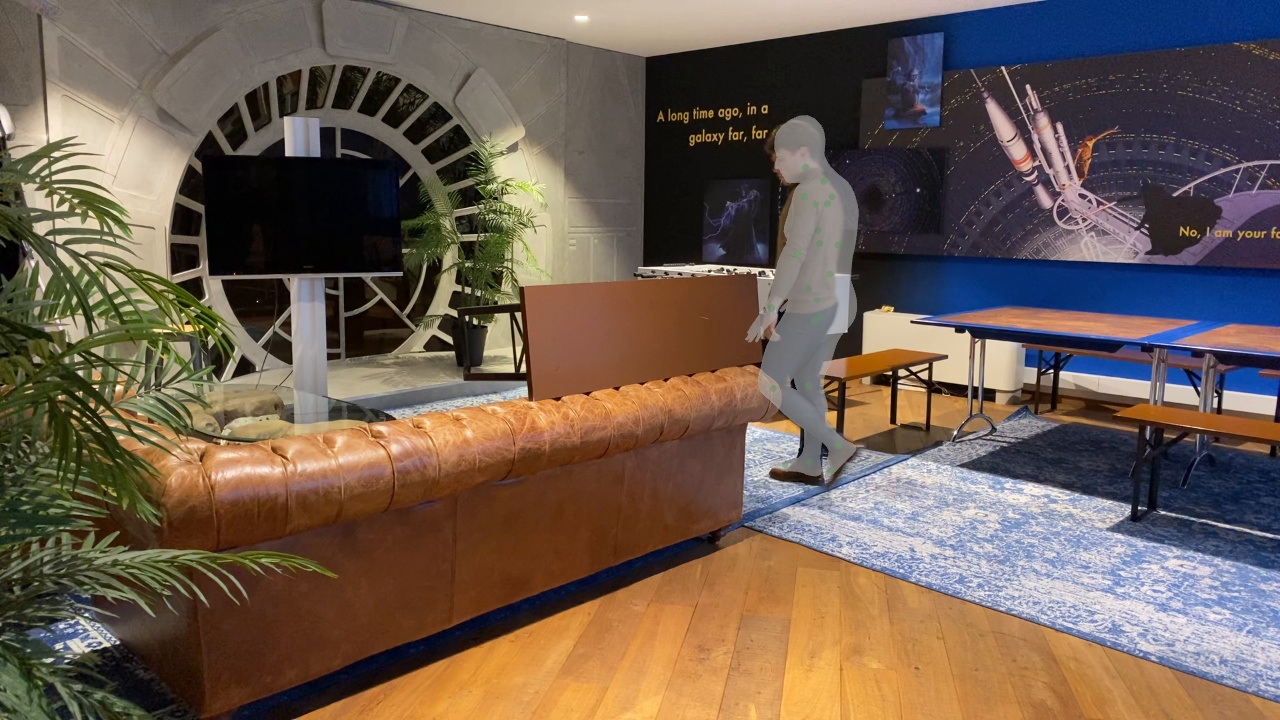
\includegraphics[width=0.3\textwidth]{Figures/humor/improvement/Rollout_stage_2/sitting_clip/stage2/frame_00000099.jpg}} 
    \hfil
    \subfloat[]{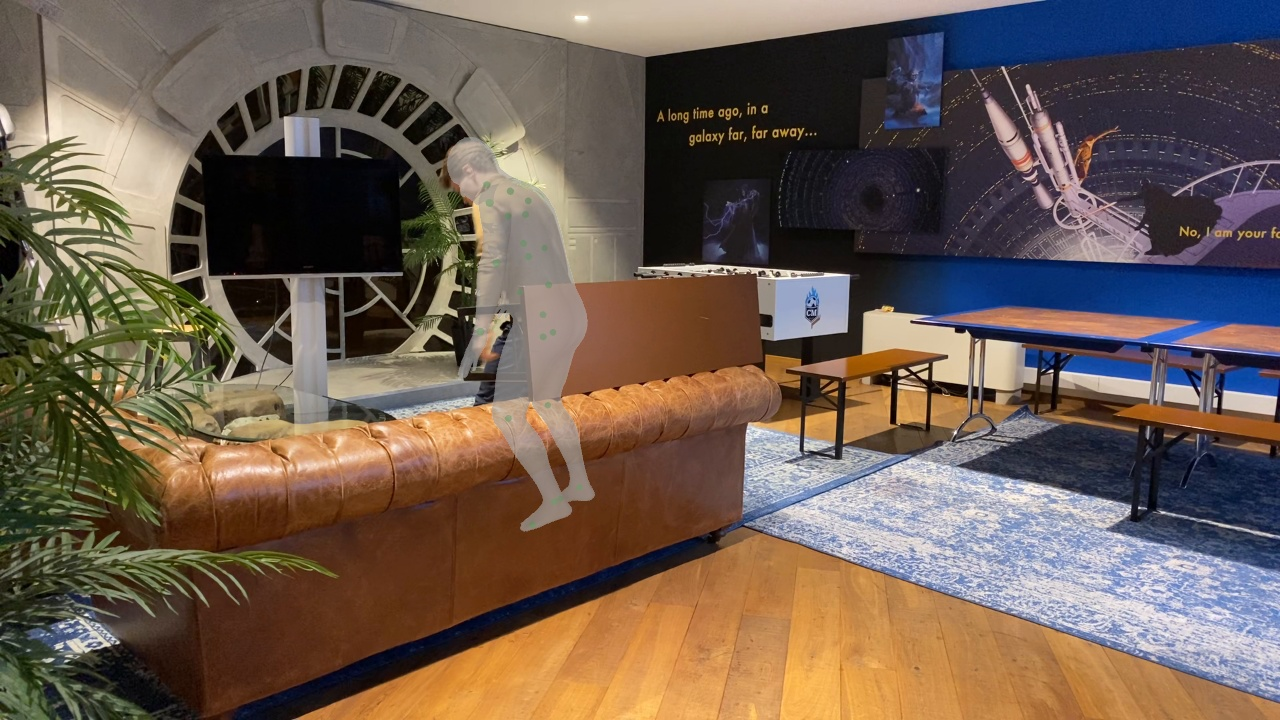
\includegraphics[width=0.3\textwidth]{Figures/humor/improvement/Rollout_stage_2/sitting_clip/stage2/frame_00000149.jpg}} 
    \hfil
    \subfloat[]{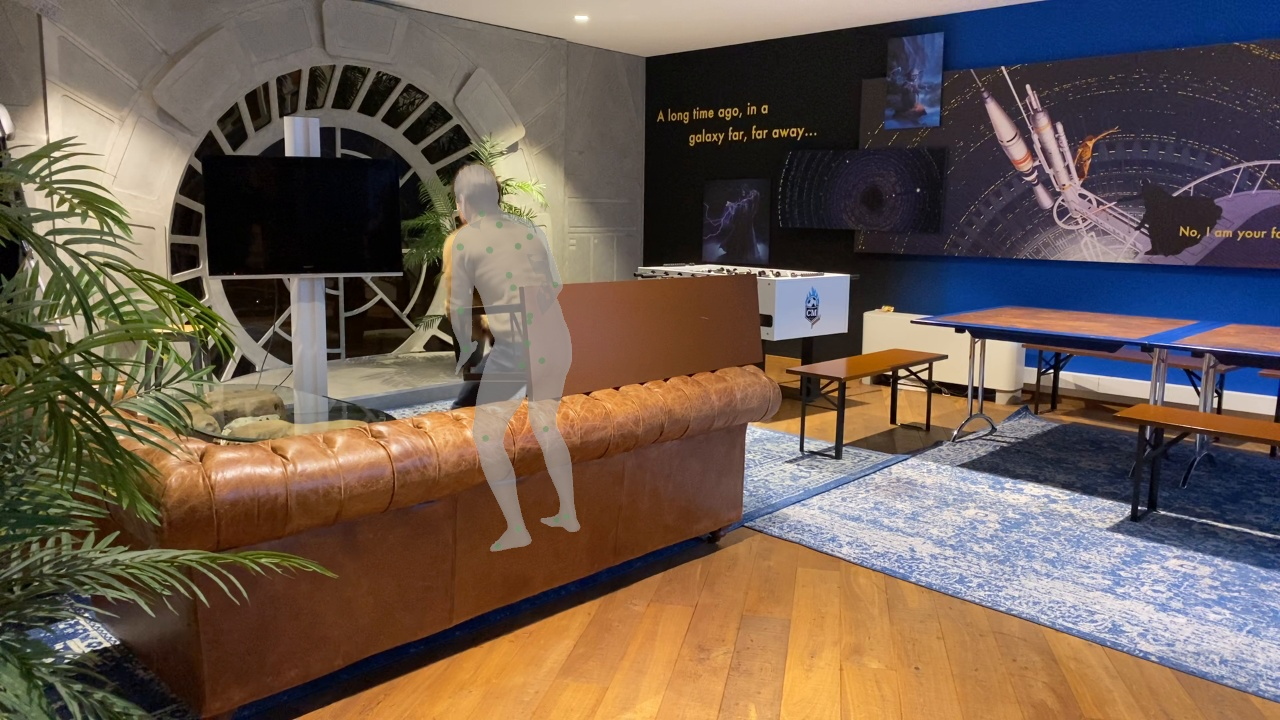
\includegraphics[width=0.3\textwidth]{Figures/humor/improvement/Rollout_stage_2/sitting_clip/stage2/frame_00000219.jpg}}
    \hfil
    \subfloat[]{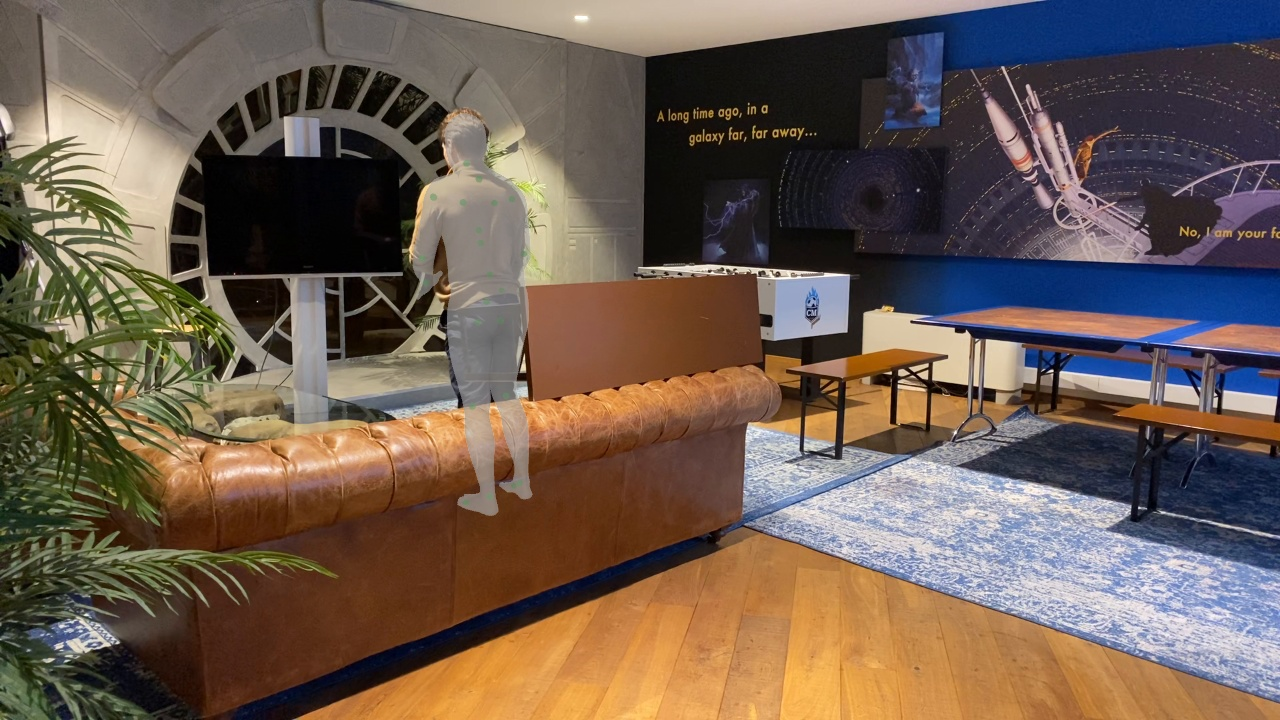
\includegraphics[width=0.3\textwidth]{Figures/humor/improvement/Rollout_stage_2/sitting_clip/stage2/frame_00000239.jpg}}
    \caption{Stage 2 $x$'s}
    \label{fig:humor_stage_2}
\end{figure}

\begin{figure}[!ht]
    \centering
    \subfloat[]{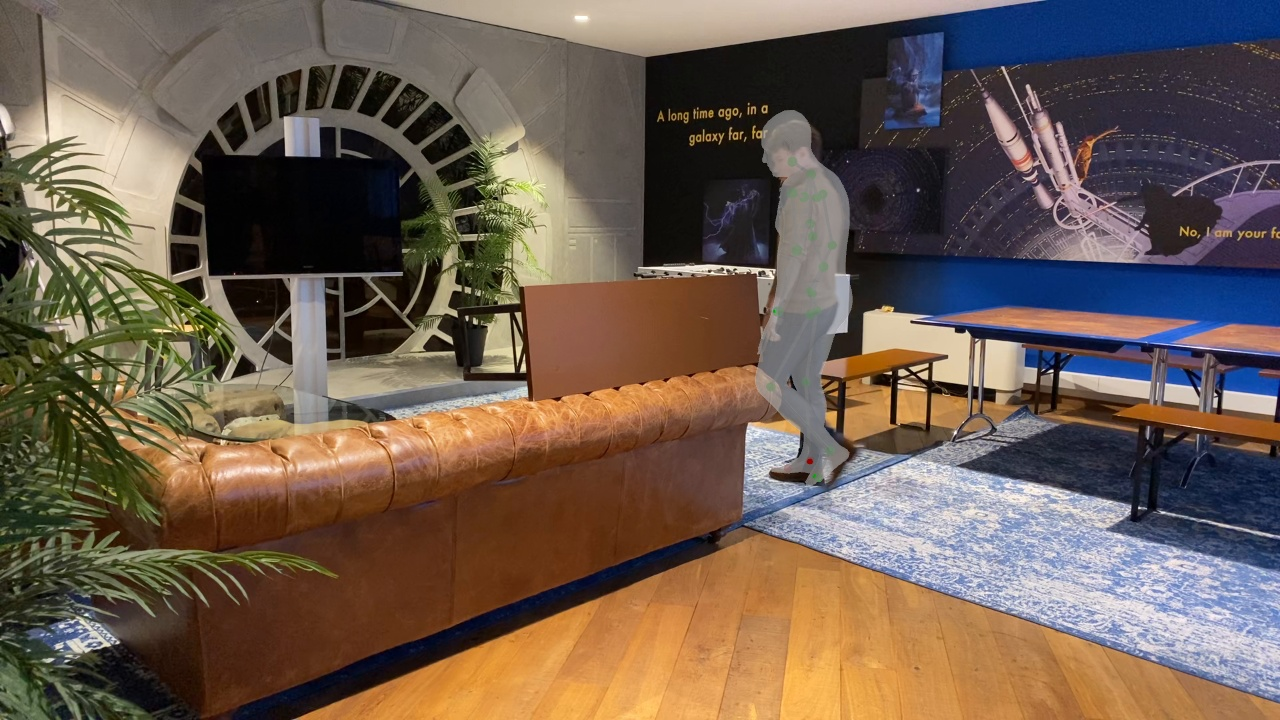
\includegraphics[width=0.3\textwidth]{Figures/humor/improvement/Rollout_stage_2/sitting_clip/rollout/frame_00000010.jpg}} 
    \hfil
    \subfloat[]{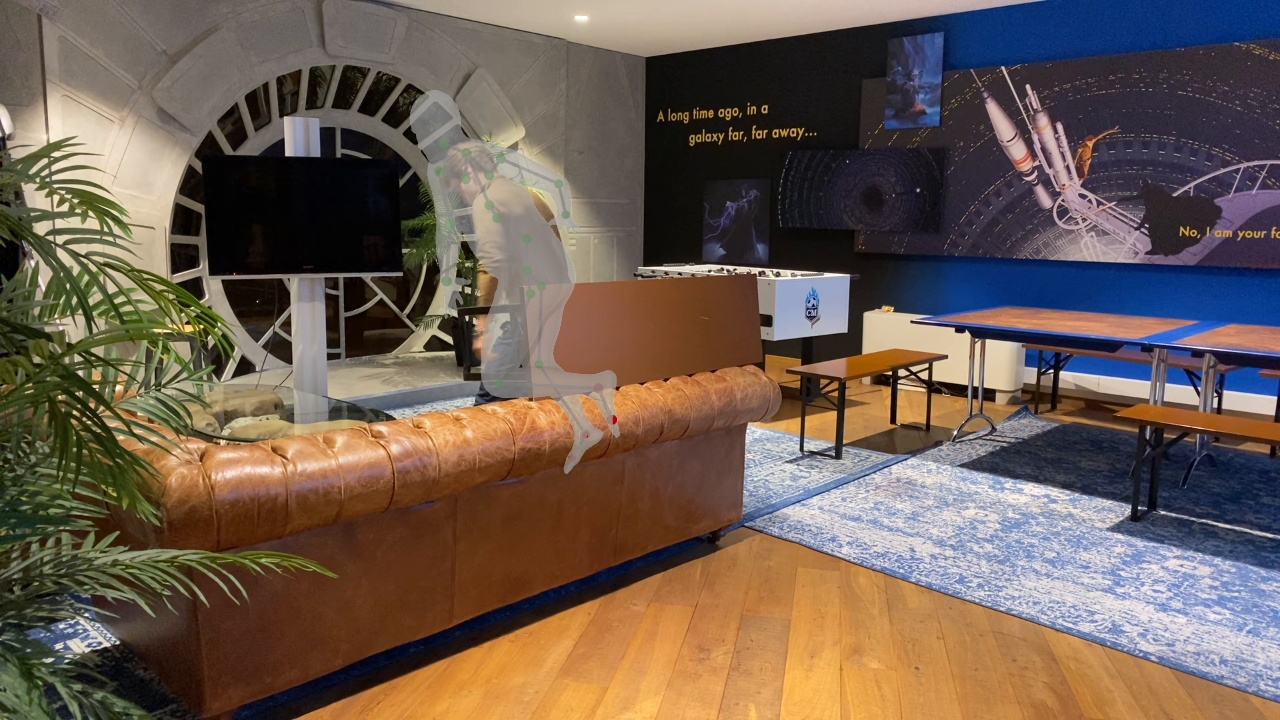
\includegraphics[width=0.3\textwidth]{Figures/humor/improvement/Rollout_stage_2/sitting_clip/rollout/frame_00000060.jpg}} 
    \hfil
    \subfloat[]{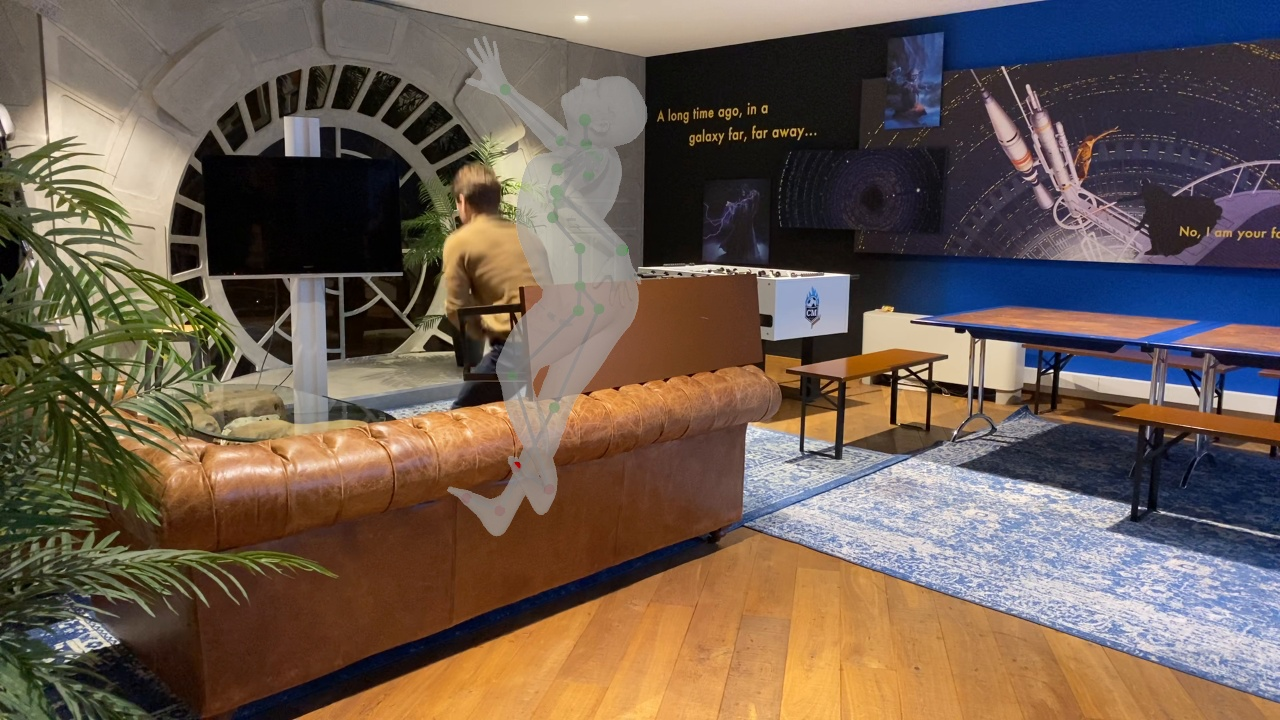
\includegraphics[width=0.3\textwidth]{Figures/humor/improvement/Rollout_stage_2/sitting_clip/rollout/frame_00000130.jpg}}
    \hfil
    \subfloat[]{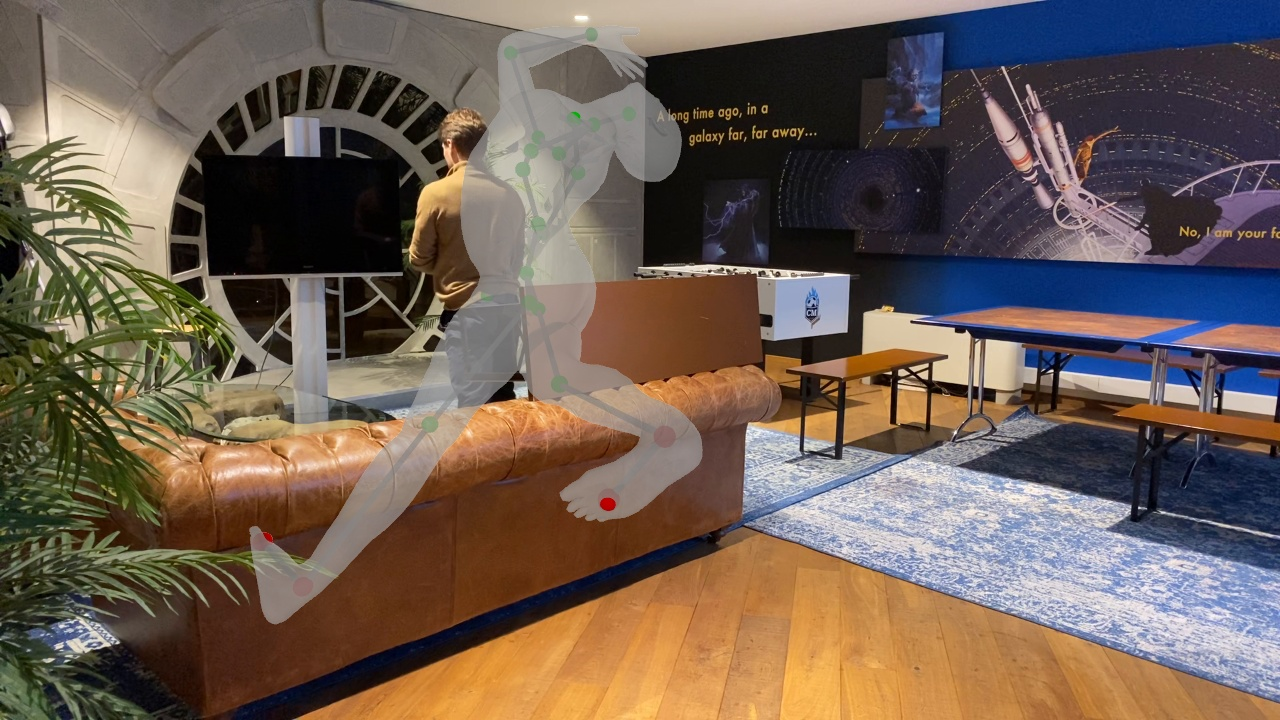
\includegraphics[width=0.3\textwidth]{Figures/humor/improvement/Rollout_stage_2/sitting_clip/rollout/frame_00000150.jpg}}
    \caption{Deviation due to rollout of Stage 2 $z$'s}
    \label{fig:humor_stage_2_rollout_deviation}
\end{figure}


With some preliminary experiments in which we began optimising $x$'s and $z$'s we found that the most successful approach to blending the decoded and optimised $x$'s was to have an L1 loss on the distance between them. We saw that when simply copying over, the propagation of small errors forward was too strong (as desribed in \figref{fig:humor_stage_2_rollout_deviation}) and the system failed to recover as the long range gradients present in the HuMoR TestOps method weren't present, and we found when blending rather than completely copying over that the weighting of the blending was another parameter that was difficult to choose, hence having a loss was the path of least resistence.

Next we experimented with jointly optimising $x$ and $z$ with a larger variety of losses. It was noted that the sitting down motion was not acheived consistenly. However as previously mentioned, the initial $z$'s encode a sitting motion, thus we conject that the $x$'s and $z$'s were fighting and this sitting motion was lost, that is to say the $z$'s move to match the $x$'s motion in which the skeleton simply clips into the floor without bending legs, thus the $z$'s begin encoding less leg bending. To avoid this issue in future experiments, the $z$'s were detached from the consistency loss making the optimised $x$'s match the decoded $x$'s.

This led us on to some experiments in which we either optimise $z$ whilst fixing $x$, or vice versa. With the $z$'s fixed at the stage 2 results, we managed to acheive a sensible sitting motion for a clip containing occluded sitting, but when we applied the same optimiser settings to a longer clip the results were no longer satisfactory. We also noted that when it did work, it required a large number of iterations, in the 1000s, which took 10mins or more, thus the speedup was not as evident as hoped (though our method would continue scaling better). In the inverse case, fixing $x$ to the final HuMoR optimised states and optimising $z$, we noted that we consistently converge in the direction of the final HuMoR $z$'s, which indicates that we are optimising in the right direction, with the best results acheived at a rollout of 5 decoding steps.

All these experiments were performed with varying numbers of decoding steps, 1, 2, 5, and 10. We found that the effect of more stable results but slower compute times with longer rollouts did manifest as intuition would suggest. 

These experiments suggest that the next direction to pursue would be an optimisation scheme in which we flip flop optimising $z$ then $x$. However considering our difficulty in achieving consistent results for the optimisation of the $x$'s with fixed $z$'s, our feeling that this might not be the optimal solution to the problem, my desire to try a new direction, and the time constraints, we deemed it time to move on and try a new method.

\subsection{Conclusion}

We found that jointly optimising the $x$'s and $z$'s did not prove an easy task to solve, which may indicate that
\begin{itemize}
    \item it is a particularly difficult problem, and therefore that the optimiser struggles to satisfy the constraints and find a good minimum for both $x$ and $z$ at the same time
    \item the coupling of the $x$'s and $z$'s in the HuMoR decoder is an important issue. We found it to be at least a minor issue as it was necessary to decouple the $z$'s from the consistency loss (matching the optimised $x$s to the decoded $x'$'s) to avoid the $z$'s being modified in such a way as to fit the unoptimised $x$'s at the beginning of the optimisation
    \item the optimiser is badly balanced
\end{itemize}
This at the very least suggests that a new decoder that does not couple $x$'s and $z$'s would be useful and worth investigating if a similar method is pursued.

In the investigations we found it possible to acheive sensible results on a given clip (for example fixing the unoptimised initial $z$'s, we can a plausible sitting motion in a small video of sitting in occlusion) but that the same settings for the optimiser failed to acheive a good result on an alternative clip. This may indicate that 
\begin{itemize}
    \item again, this is a difficult problem that the optimiser will struggle to solve
    \item the optimiser is badly balanced
\end{itemize} as before.

While many of the issues encountered may simply be due to a badly balanced optimiser, considerable effort was made to mitigate this potential issue, and therefore it is our impression that this problem is at the very least a difficult one. We have improved our intuition, fixed several issues, and understood more about the problem and our goals. We therefore can make a more informed decision with respect to which direction to pursue next. \\
We found that taking a system that was designed with autogregression in mind, and trying to parrallelise it, proved more difficult than expected. The experiments lead us to beleive that jointly optimising a sequence of poses and latent variables obtained through a single frame decoder may be a more difficult formulation of the problem than others. We therefore conclude that a method in which we model longer motion sequences may be more fruitful.

\TODO{Double check through Notes/Current\_experiments.md to see if there's anything else we can learn from the experiments}
\chapter{Motion Diffusion Models}

\section{Method}

%%%%%%%%%%%%%%%%%%%%%%%%%%%%%%%%%%%%%%%%%%%%%%%%%%%%%%%%%%%%%%%%%%%%
% General diffusion models
%%%%%%%%%%%%%%%%%%%%%%%%%%%%%%%%%%%%%%%%%%%%%%%%%%%%%%%%%%%%%%%%%%%%
\subsection{Diffusion Models}
\label{sec:diffusion_models}
The diffusion framework that we use is defined theoretically as follows \cite{ddpm,improved_diffusion,EDGE}. Given $x_0 \sim p(x_0)$ from some data distribution, diffusion is a Markov noising process over latent variables $x_t, t=1,...,T$. The process of adding noise (the 'forward noising process') is defined through the distributions
\begin{equation}
    \begin{aligned}
        q(x_t|x_{t-1}) &:= \mathcal{N}(\sqrt{1-\beta_t} x_{t-1}, \beta_t \mathbf{I}) \\
        q(x_T | x_0) &:= \prod_{t=1}^T q(x_t | x_{t-1}) \\
    \end{aligned}
\end{equation}
. With a well-chosen variance schedule $\beta_1, ..., \beta_T$ and a large T, we approximate a standard normal distribution as we approach $t=T$. This entails that the first latent variable $x_T$ is approximately Gaussian noise. The 'reverse noising process' is unknown without the full data distribution, which we don't have access to, hence we approximate it using some parametrized function
\begin{equation}
    \label{eq:reverse_noising_mean_variance}
    p_{\theta}(x_{t-1} | x_t) = \mathcal{N}(\mu_{\theta}(x_t, t), \Sigma_{\theta}(x_t, t))
\end{equation}

The whole process can be visualized in \figref{fig:diffusion_process} borrowed from the DDPM paper \cite{ddpm}.

\begin{figure}[!ht]
    \centering
    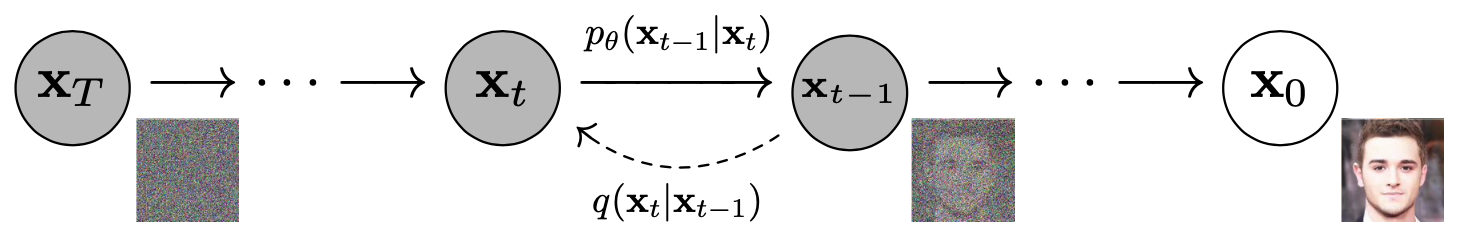
\includegraphics[width=0.75\textwidth]{Figures/diffusion/diffusion_process.png}
    \caption{Diffusion Process}
    \label{fig:diffusion_process}
\end{figure}

We find with $p$ and $q$ that this system forms a VAE that can be trained through the Variational Lower Bound (VLB) \cite{kingma2022_VAE}.

In practice, however, some modifications are commonly made to this definition to ease our implementation and improve performance.
Firstly we note that the forward noising process can be written as
\begin{equation}
    \label{eq:direct_noising_latents}
    q(x_t|x_0) \sim \mathcal{N}(\sqrt{\bar{\alpha_t}}x_0, (1-\bar{\alpha_t})\mathbf{I})
\end{equation}
with $\bar{\alpha_t} = \prod_{s=1}^t \alpha_s$ and $\alpha_t = 1 - \beta_t$. This is simply a mixing of the data with Gaussian noise according to a monotonically decreasing schedule $\bar{\alpha_t}$ and allows us to sample any latent variable at any timestep directly from the clean signal, which aids the training procedure described in \secref{sec:diffusion_training}. Next, we also note that we take the following definition for the $\bar{\alpha_t}$ schedule (rather than defining the $\beta$ schedule), as in \cite{improved_diffusion},
\begin{equation}
    \begin{aligned}
    \bar{\alpha_t} &= \frac{f(t)}{f(0)} \\
    f(t) &= \cos \left( \frac{t/T + s}{1 + s} \cdot \frac{\pi}{2} \right)
    \end{aligned}
\end{equation}
with a small offset $s$ (we take $s=0.008$ \cite{improved_diffusion}) to avoid $\beta_t$ from being too small near $t=0$ which can reduce performance, according to the authors.

We also use a simplified reverse noising process, where rather than predicting the mean and variance of the noise for a single step as indicated in \eqref{eq:reverse_noising_mean_variance}, we directly try to predict the denoised signal \cite{ramesh2022hierarchical},
\begin{equation}
    \label{eq:denoised_signal_prediction}
    \hat{x}_{\theta}(x_t, t) \approx x_0 \\
\end{equation}
which, alongside the choice of a fixed rather than learned variance as in \cite{ddpm}, allows us to describe the denoising process as follows, where a tractable expression is provided by Bayes Theorem \cite{improved_diffusion},
\begin{equation}
    \label{eq:direct_prediction_denoising}
    \begin{aligned}
    p_{\theta}(x_{t-1} | x_t) &= q\big(x_{t-1} | x_t, \hat{x}_{\theta}(x_t, t)\big)  \\
    &= \mathcal{N}(\mu_{\theta}(x_t, t), \tilde{\beta}_t I)
    \end{aligned}
\end{equation}
with 
\begin{equation}
    \label{eq:direct_prediction_denoising_details}
    \begin{aligned}
    \tilde{\beta}_t &= \frac{1 - \bar{\alpha}_{t-1}}{1 - \bar{\alpha}_t} \beta_t \\
    \mu_{\theta}(x_t, t) &= \frac{\sqrt{\bar{\alpha}_{t-1}}\beta_t}{1-\bar{\alpha}_t}\hat{x}_{\theta}(x_t, t) + \frac{\sqrt{\alpha}_t(1-\bar{\alpha}_{t-1})}{1-\bar{\alpha}_t}x_t
    \end{aligned}
\end{equation}
.
This direct prediction of the denoised signal allows us to use the simplified MSE objective \cite{ddpm,ramesh2022hierarchical} during training
\begin{equation}
    \label{eq:simple_loss}
    \mathcal{L}_{simple} = \mathbb{E}_{x_0,t}\left[ \| x_0 - \hat{x}_{\theta}(x_t, t) \|_2^2 \right]
\end{equation}
which can still be interpreted as a form of Variational Lower Bound without the variance terms.

The essential idea of training such a model is to randomly sample a timestep, noise a signal back to this timestep with \eqref{eq:direct_noising_latents}, predict the denoised signal with \eqref{eq:denoised_signal_prediction}, and perform a backward step on the loss described in \eqref{eq:simple_loss} alongside some other regularisation losses that suit our problem.

The inference procedure involves sampling random Gaussian noise, then iteratively predicting the denoised signal with \eqref{eq:denoised_signal_prediction} and sampling from the next timestep with \eqref{eq:direct_prediction_denoising}.

%%%%%%%%%%%%%%%%%%%%%%%%%%%%%%%%%%%%%%%%%%%%%%%%%%%%%%%%%%%%%%%%%%%%
% Our diffusion model
%%%%%%%%%%%%%%%%%%%%%%%%%%%%%%%%%%%%%%%%%%%%%%%%%%%%%%%%%%%%%%%%%%%%
\subsection{Model Design}
\label{sec:disney_motion_diffusion}
Armed with this understanding of diffusion, we move on to the task of designing our model, strongly inspired by the work of Tevet. et. al \cite{MDM}.


\subsubsection{State Representation}
\label{sec:diffusion_state_representation}
Our state represents a motion sequence of length $N$, and includes primarily a root translation, $r \in \mathbb{R}^{N \cross 3}$, and 6d \cite{aa_6d_angles} joint orientations in body frame, $o \in \mathbb{R}^{N \cross 6}$. The state can be extended with some optional extras, depending on the data, of foot ground contacts $b \in \mathbb{R}^{N \cross 1}$, and explicit velocities for the root translation and joint orientations. Again, depending on the data, we can represent the root translation, and root orientations (a subset of the joint orientations) either in world space, where each motion sequence will have a distinct starting point and starting orientation or as what we call a 'stuck root' reference frame, where the first pose is set to the positions $(0,0)$ and identity root orientation and all subsequent poses are described with respect to this first frame, with the idea being that this formulation leads to a smaller space for the model to learn.


\subsubsection{Architecture}
We follow closely \cite{MDM} in our architecture, though without the text conditioning. We use a simple transformer \cite{vaswani2017attention} encoder as the denoising network, conditioned on the diffusion timestep so that the network can learn how much noise is present that needs removing. This is used with the described denoising process which can be seen in \figref{fig:dmd_architecture}.

\begin{figure}[!ht]
    \centering
    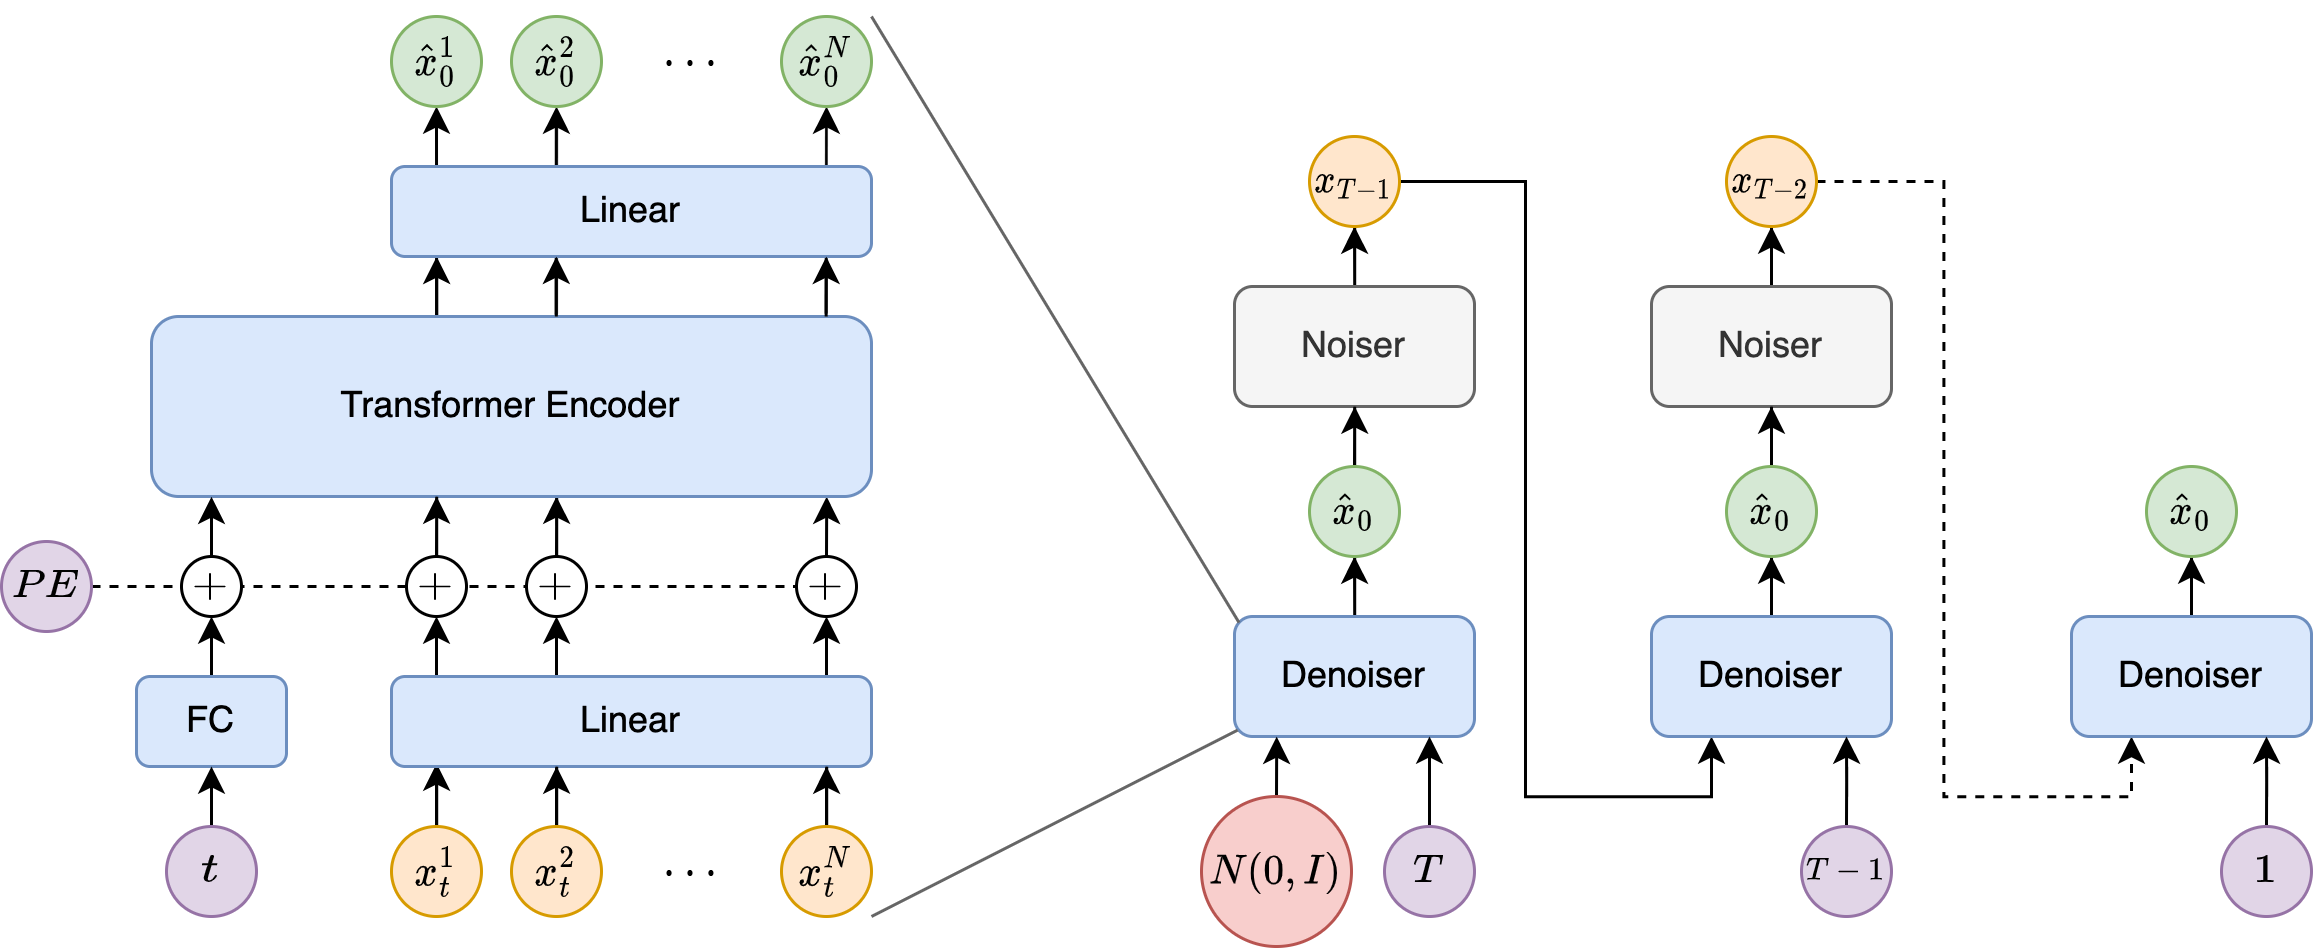
\includegraphics[width=1\textwidth]{Figures/diffusion/Network_diagram.png}
    \caption{Model Architecture \& Denoising Process}
    \label{fig:dmd_architecture}
\end{figure}



\subsubsection{Training}
\label{sec:diffusion_training}

In addition to the simple MSE loss described in section \ref{sec:diffusion_models}, we can include a number of other losses to aid the training procedure.
\begin{equation}
    \begin{aligned}
        \mathcal{L}_{fk} &= \frac{1}{N} \sum_{i=1}^{N} \| x_0^{(pos)} - FK(\hat{x}_0^{(i)})  \|_2^2 \\
        \mathcal{L}_{vel} &= \frac{1}{N-1} \sum_{i=1}^{N-1} \| (x_0^{(i+1)} - x_0^{(i)}) - (\hat{x}_0^{(i+1)} - \hat{x}_0^{(i)}) \|_2^2 \\
        \mathcal{L}_{contact} &= \frac{1}{N-1} \sum_{i=1}^{N-1} \| \left( FK(\hat{x}_0^{(i+1)}) - FK(\hat{x}_0^{(i)}) \right) \cdot \hat{b}^{(i)}  \|_2^2
    \end{aligned}
\end{equation}
with $x_0^{(i)}$ representing the $i$th pose of the motion sequence $x_0$. The $\mathcal{L}_{fk}$ loss is a forward kinematics loss, i.e a loss on the positions that are calculated from the orientations through a forward kinematic function and compared to the ground truth positions that we have access to, $x_0^{(pos)}$, and which provides another mechanism by which the orientations might be adjusted, thus increasing the robustness of the predictions. The $\mathcal{L}_{vel}$ loss is a calculated velocity loss, in which the first-order finite differences are used to estimate the velocities of the state (orientations and root translation only in this case), and which encourages the model to learn a smooth motion sequence. The $\mathcal{L}_{contact}$ loss is a foot contact loss, where the velocities of the ground-contacting feet joints, indicated by the predicted foot contacts $\hat{b}^{(i)}$, are minimised so as to discourage foot sliding. We note that the $\mathcal{L}_{contact}$ loss is only used when the ground contacts are included in the state representation.



\subsubsection{Inpainting}
\label{sec:diffusion_method_inpainting}

An important tool in the arsenal of the diffusion model literature is that of inpainting \cite{diffusion_inpainting}. Inpainting is the process of keeping a portion of the state constant throughout the diffusion process. An example of the use of this technique would be that of changing the motion of the lower body while maintaining the motion of the upper body, though many other use cases are explored in more detail in \secref{sec:diffusion_experiments}. The inpainting procedure works as follows; at each denoising step we mix a portion of the latent variable state $\hat{x}_t$, indicated through the binary mask $m$, with the complementary portion of some known state $x^{(known)}$, indicated through $1-m$, 
\begin{equation}
    \hat{x}_{t} = m \odot \hat{x}_t + (1-m) \odot q(x^{(known)}|t-1)
\end{equation}
Graphically this process can be seen in the diagram presented in \figref{fig:inpainting_diagram}, and more intuitively in \figref{fig:inpainting_video} where the inpainting progression is shown for the example of replacing leg motion. This procedure is particularly attractive as it requires no special training procedure, and can be employed readily with any diffusion model.

\begin{figure}[!ht]
    \centering
    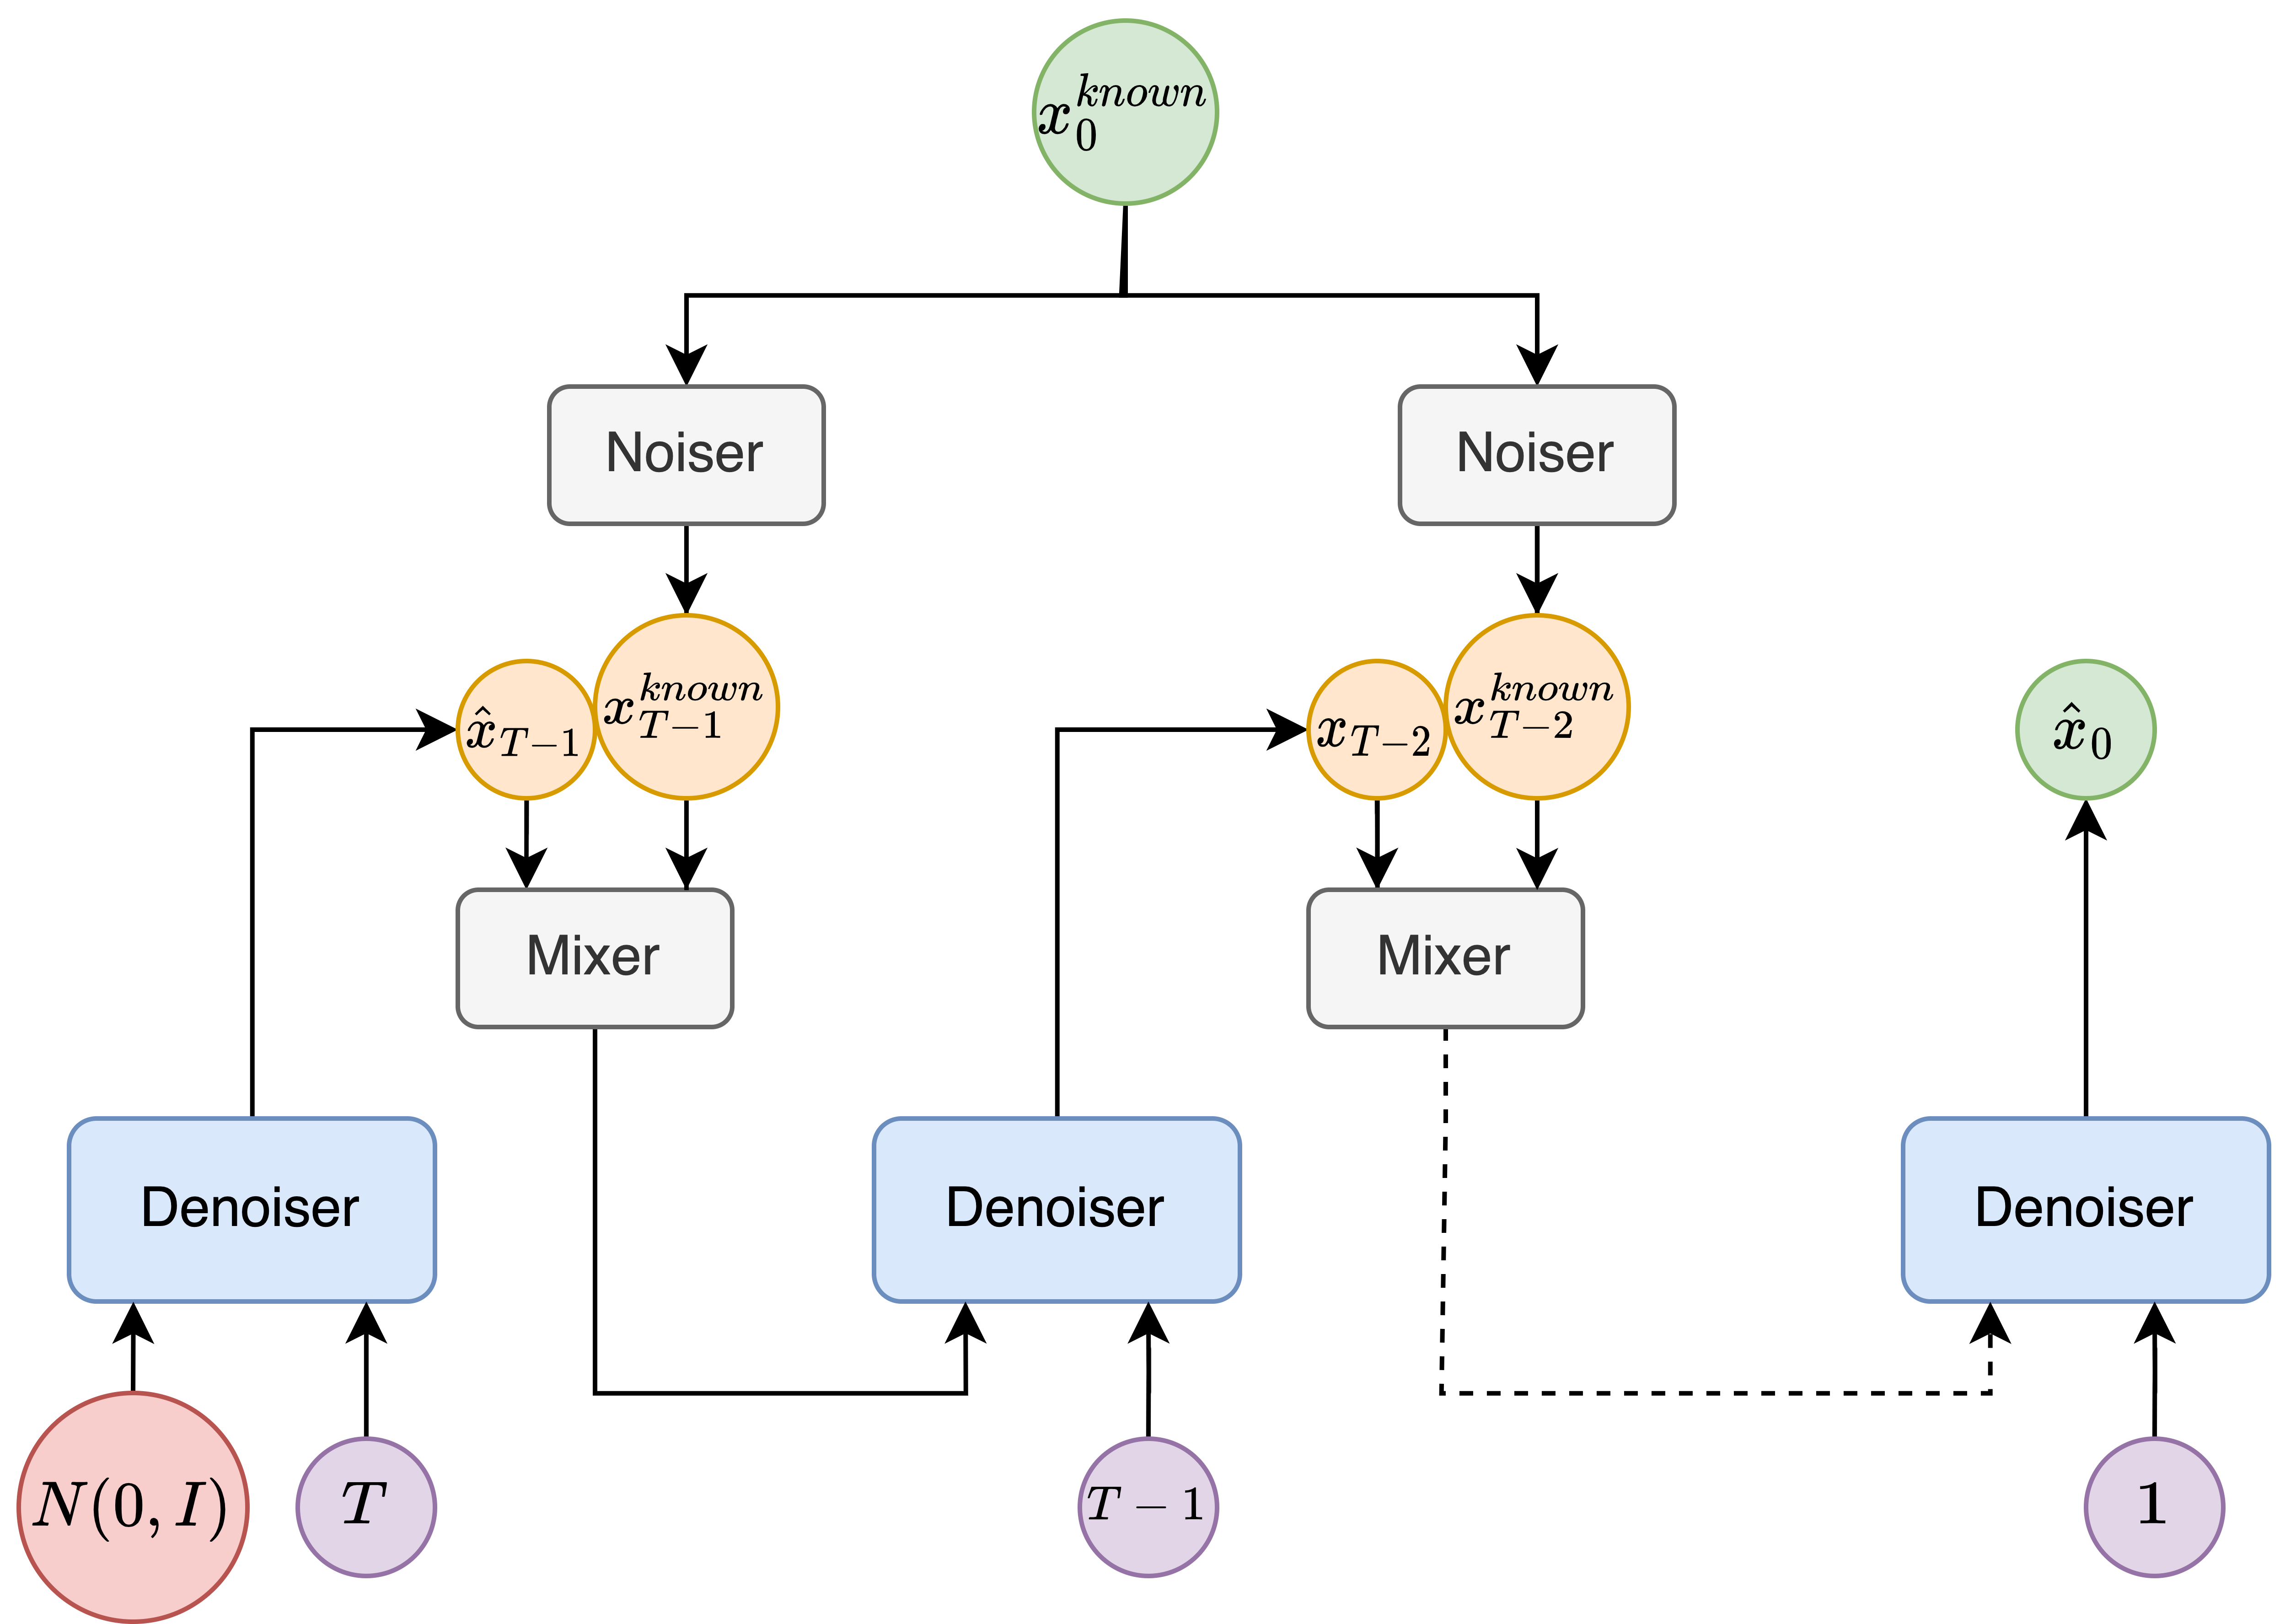
\includegraphics[width=1\textwidth]{Figures/diffusion/Inpainting.png}
    \caption{Inpainting Procedure}
    \label{fig:inpainting_diagram}
\end{figure}

\begin{figure}[!ht]
    \centering
    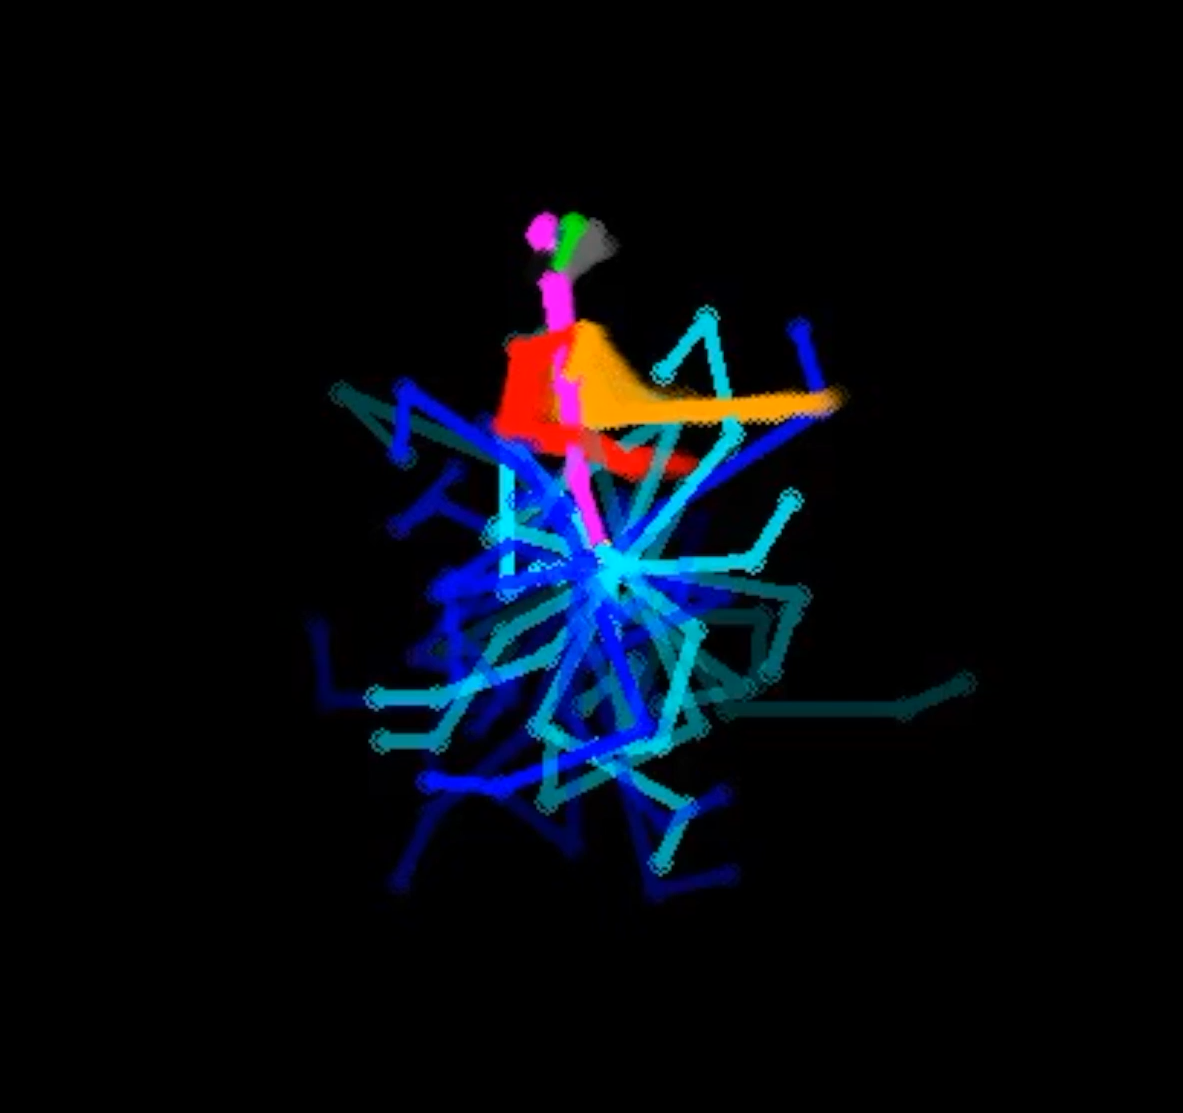
\includegraphics[width=0.2\textwidth]{Figures/diffusion/inpainting/1.png}
    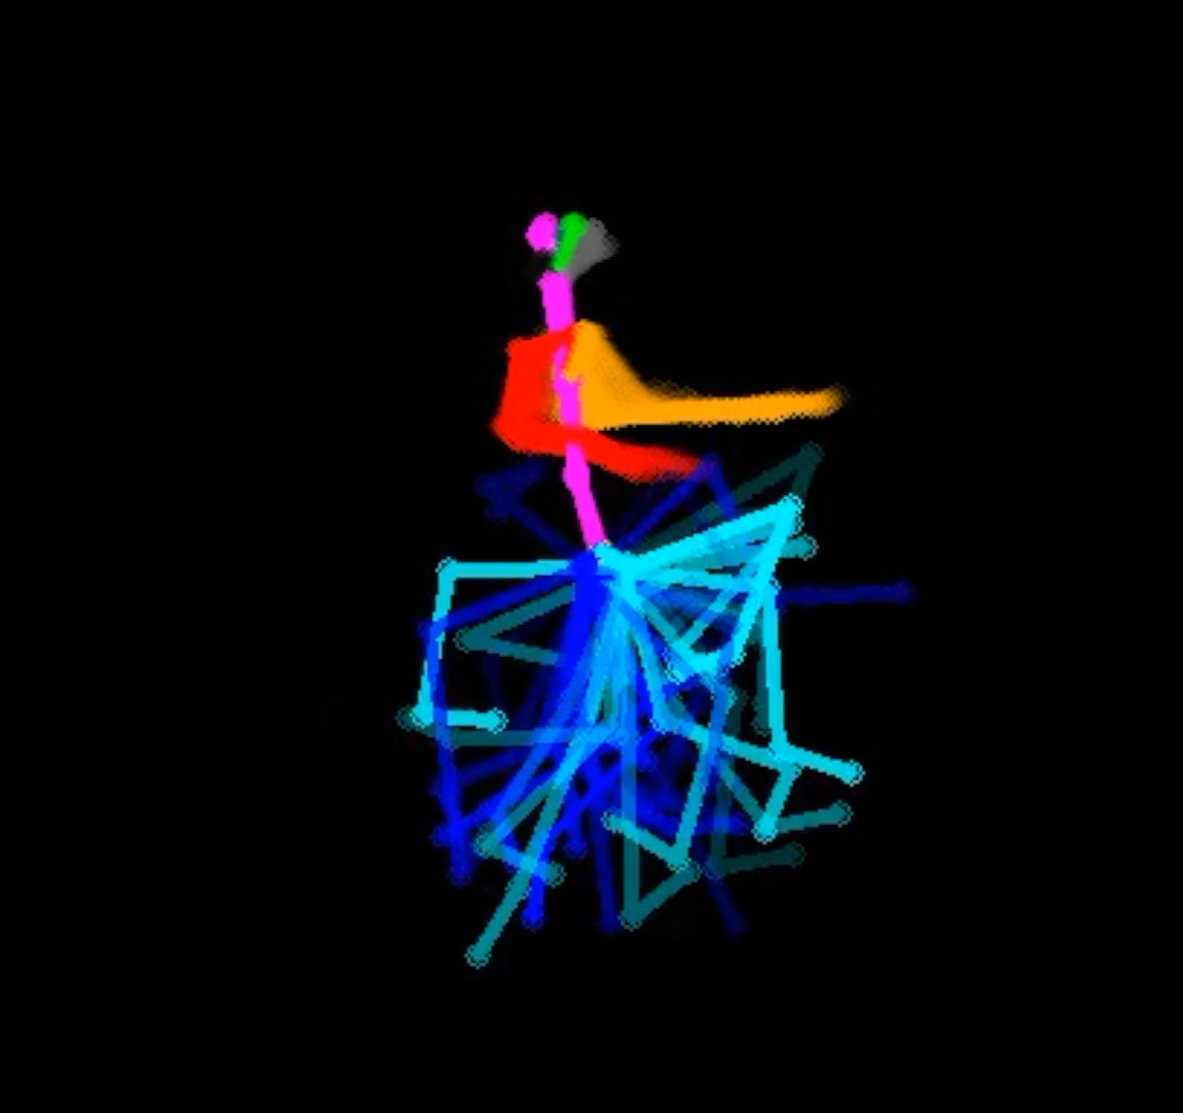
\includegraphics[width=0.2\textwidth]{Figures/diffusion/inpainting/2.png}
    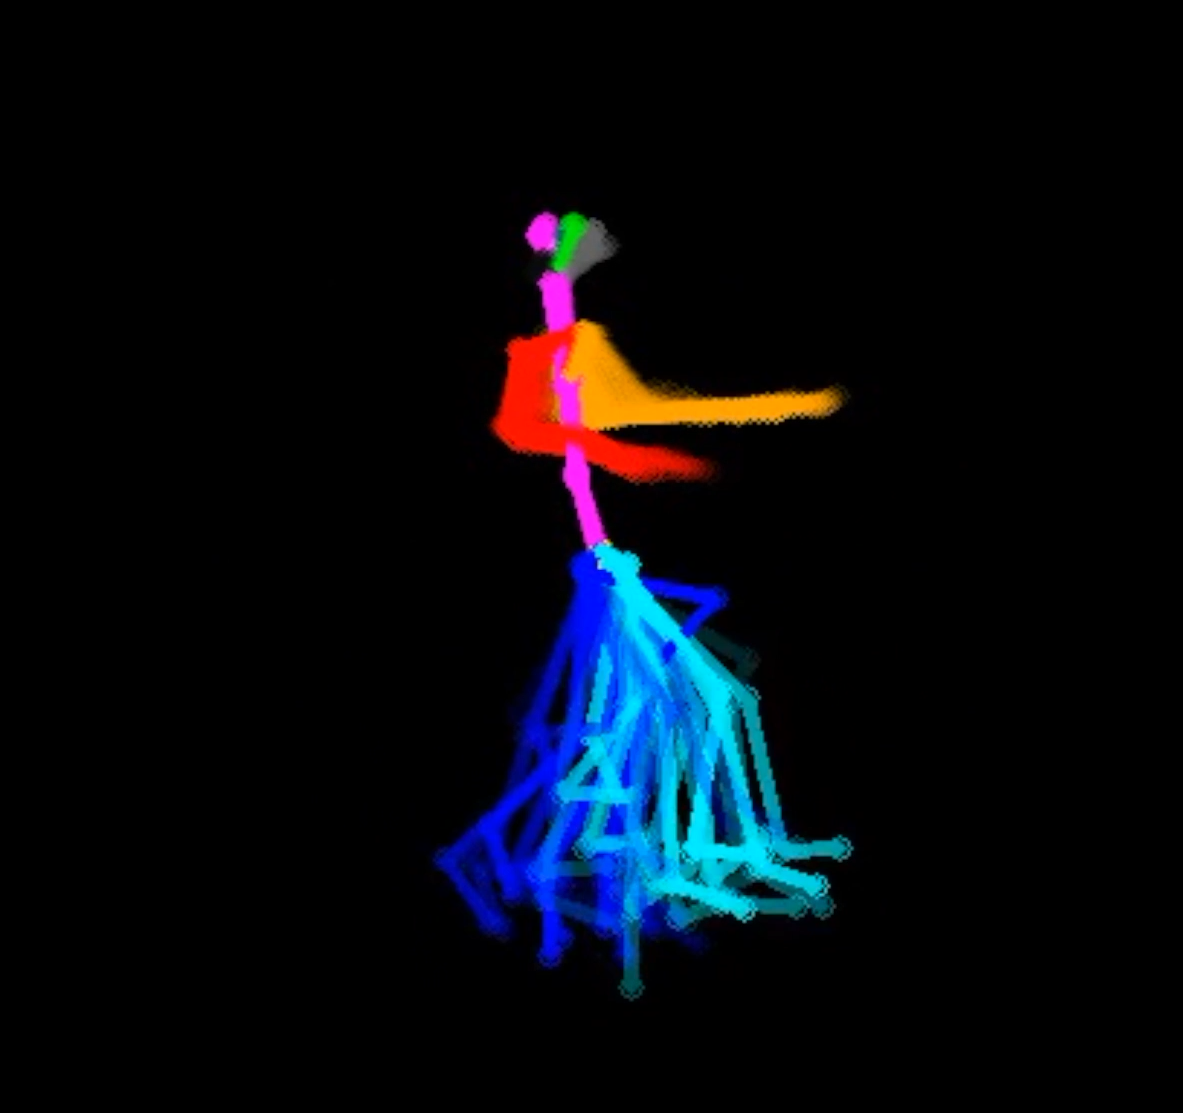
\includegraphics[width=0.2\textwidth]{Figures/diffusion/inpainting/3.png}
    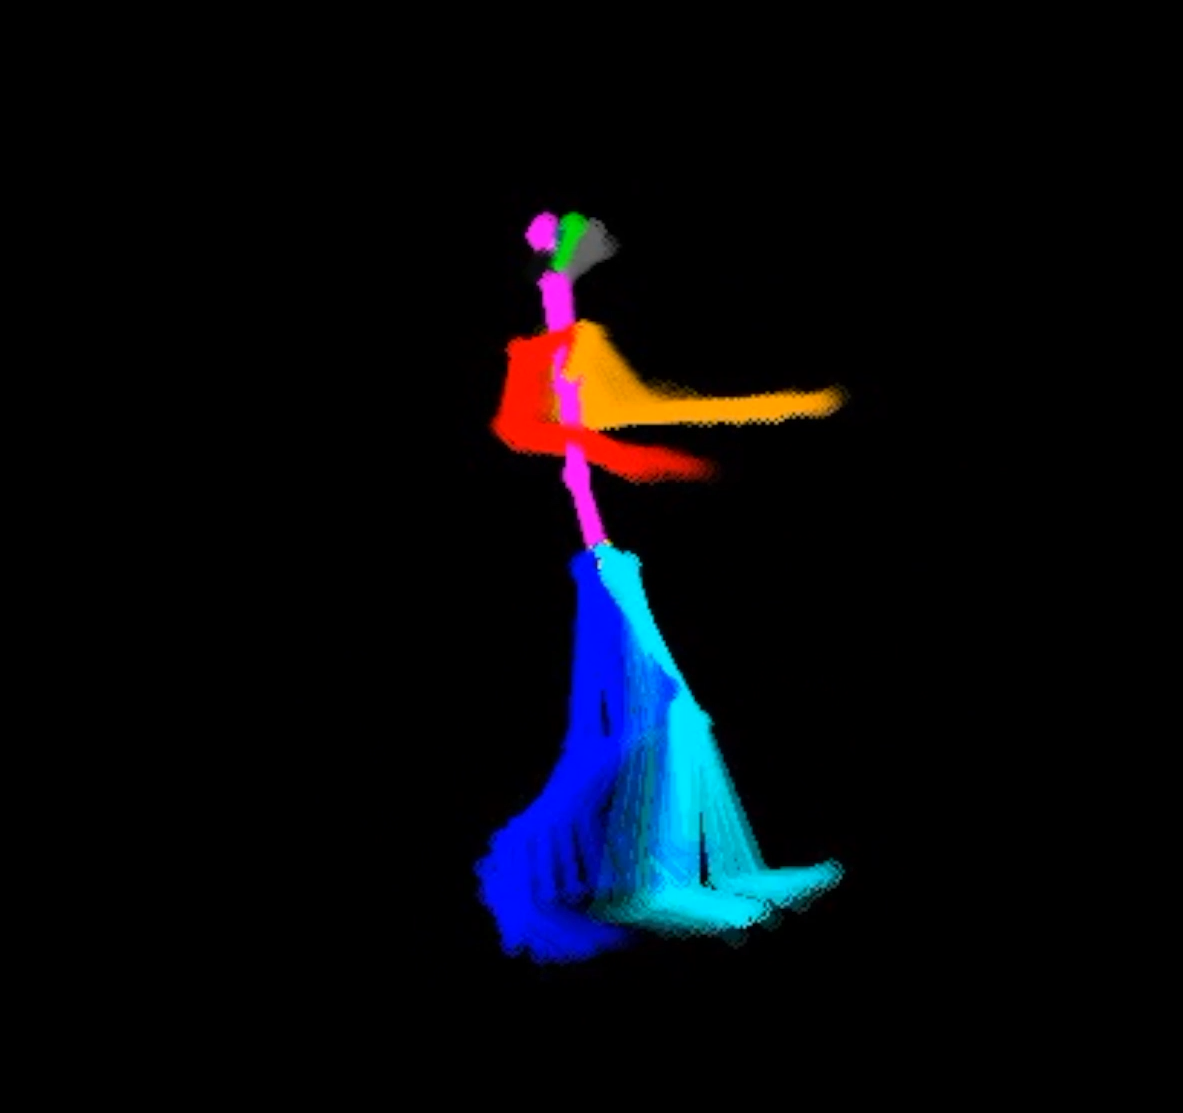
\includegraphics[width=0.2\textwidth]{Figures/diffusion/inpainting/4.png}
    \caption{Inpainting: Replacing the legs of a motion sequence}
    \label{fig:inpainting_video}
    \medskip
    \small
    \raggedright
    On the left we can see the first step of the inpainting procedure in which we have replaced the upper body and kept random noise for the lower body. As we proceed in the denoising process, we continually replace the upper body with the known fixed motion whilst denoising the legs.

    Note that these images are illustrative and intended to help the reader's intuition. In reality, the upper body is also noised to the corresponding diffusion step but we have shown the denoised version here so that it is obvious what is kept constant.
\end{figure}


\subsubsection{Data}
We have access to professional motion capture data that encompasses a wide range of possible motion for a number of subjects. In total we have 21 motion sequences on the order of 2 minutes each, thus in total we have around 45 minutes of motion capture data. This data is normalised elementwise and retargeted to a standard skeleton. Several motion sequences are held out for testing.
We have one dataset where the root of the skeleton is kept static in the y direction but can move freely in all others, and one version of the dataset that has a freely moving root and for which we have calculated foot contact labels.
\section{Experiments}
\label{sec:diffusion_experiments}

Or main goal in this investigation into diffusion models was to get a better understanding of their performance on a wide range of tasks. We keep in mind the original task of improving an existing motion sequence, but are aware of the other potentials of the model and so do not limit ourselves in scope.


%%%%%%%%%%%%%%%%%%%%%%%%%%%%%%%%%%%%%%%%%%%%%%%%%%%%%%%%%%%%%%%%%%%%%%%%%
% General test cases
%%%%%%%%%%%%%%%%%%%%%%%%%%%%%%%%%%%%%%%%%%%%%%%%%%%%%%%%%%%%%%%%%%%%%%%%%
\subsection{Test Cases}
We present here a variety of different test cases that on which the models performance can be evaluated. The general structure of the evaluation is to generate a sufficiently large number of sequences for each given task, then to import them into blender and visually inspect their quality and how well they acheive each task. We have decided to take a qualitative approach as we are attempting to get a better understanding of the models capabilities, and so this was the path of least resistance to obtain such an understanding in the time that was left after the HuMoR investigation. We note that in the future, if a given task is deemed worth investigation further, or if a significantly larger number of models are being test, more rigorous evaluation metrics would be greatly benefitial.

\subsubsection{Sequence Generation}
To ensure that the model has learned a sensible variety of human motion, we generate a number of sequences from gaussian noise, and check that they contain sufficient diversity, considering that a main indicator of an overfit diffusion model is that of a lack of diversity.

\subsubsection{Denoising}
\TODO{Come up with a better test for this}

\subsubsection{Occluded Legs}
An important situation in which the current Disney Research|Studious model does not perform optimally is that of occluded sequences. To test the ability of the diffusion models to handle this situation, we evaluate the models capabilities to generate the leg motion of an entire motion sequence. We acheive this using the inpainting framework described in \secref{sec:diffusion_method_inpainting}, keeping the upper body joint rotations and the root translation fixed, and allowing the model free reign over the rest of the state.

\subsubsection{Missing State}
To further test the ability of the models to handle occlusions, a test case where we only keep a random percent of the state during inpainting. This can either be 
\begin{enumerate}
    \item a random subset of each frame in a motion sequence
    \item a random subset that is constant across the whole sequence
\end{enumerate}
with the first testing the models ability to handle arbitrarily occuring missing data, and the second testing the models ability to recover from longer term occlusions.

\subsubsection{Inbetweening}
Another important area of motion generation research is that of Motion Inbetweening, in which the goal is to fill in a middle part of a motion sequence in which a number of frames at the beginning and end of the sequence are given. Again we can use the inpainting framework from \secref{sec:diffusion_method_inpainting} and keep the edges of the motion as static.


%%%%%%%%%%%%%%%%%%%%%%%%%%%%%%%%%%%%%%%%%%%%%%%%%%%%%%%%%%%%%%%%%%%%%%%%%
% Baseline model
%%%%%%%%%%%%%%%%%%%%%%%%%%%%%%%%%%%%%%%%%%%%%%%%%%%%%%%%%%%%%%%%%%%%%%%%%
\subsection{Baseline Model}
\label{sec:baseline_evaluation}
The baseline model was trained with the Disney Research|Studios dataset that does not, and cannot (due to a lossy rendering of the mocap), contain foot contacts. The state includes the root translation, joint orientations, and their respective velocities explicitly. It was trained for \TODO{X} epochs. \TODO{More details?}

\subsubsection{Sequence Generation}
We found that the model generates a diverse set of plausible motion, a number of frames are shown in \figref{fig:baseline_generation}. A few shortcomings however can be seen. Most notably we find that the model produces a fair bit of foot sliding \TODO{Is this true??}, where the foot seem to be in contact with the ground but has a non zero velocity in some directions. This effect can be mitigated through the use of the foot sliding loss coupled with data with containing labeled foot contacts.

\begin{figure}[!ht]
    \centering
    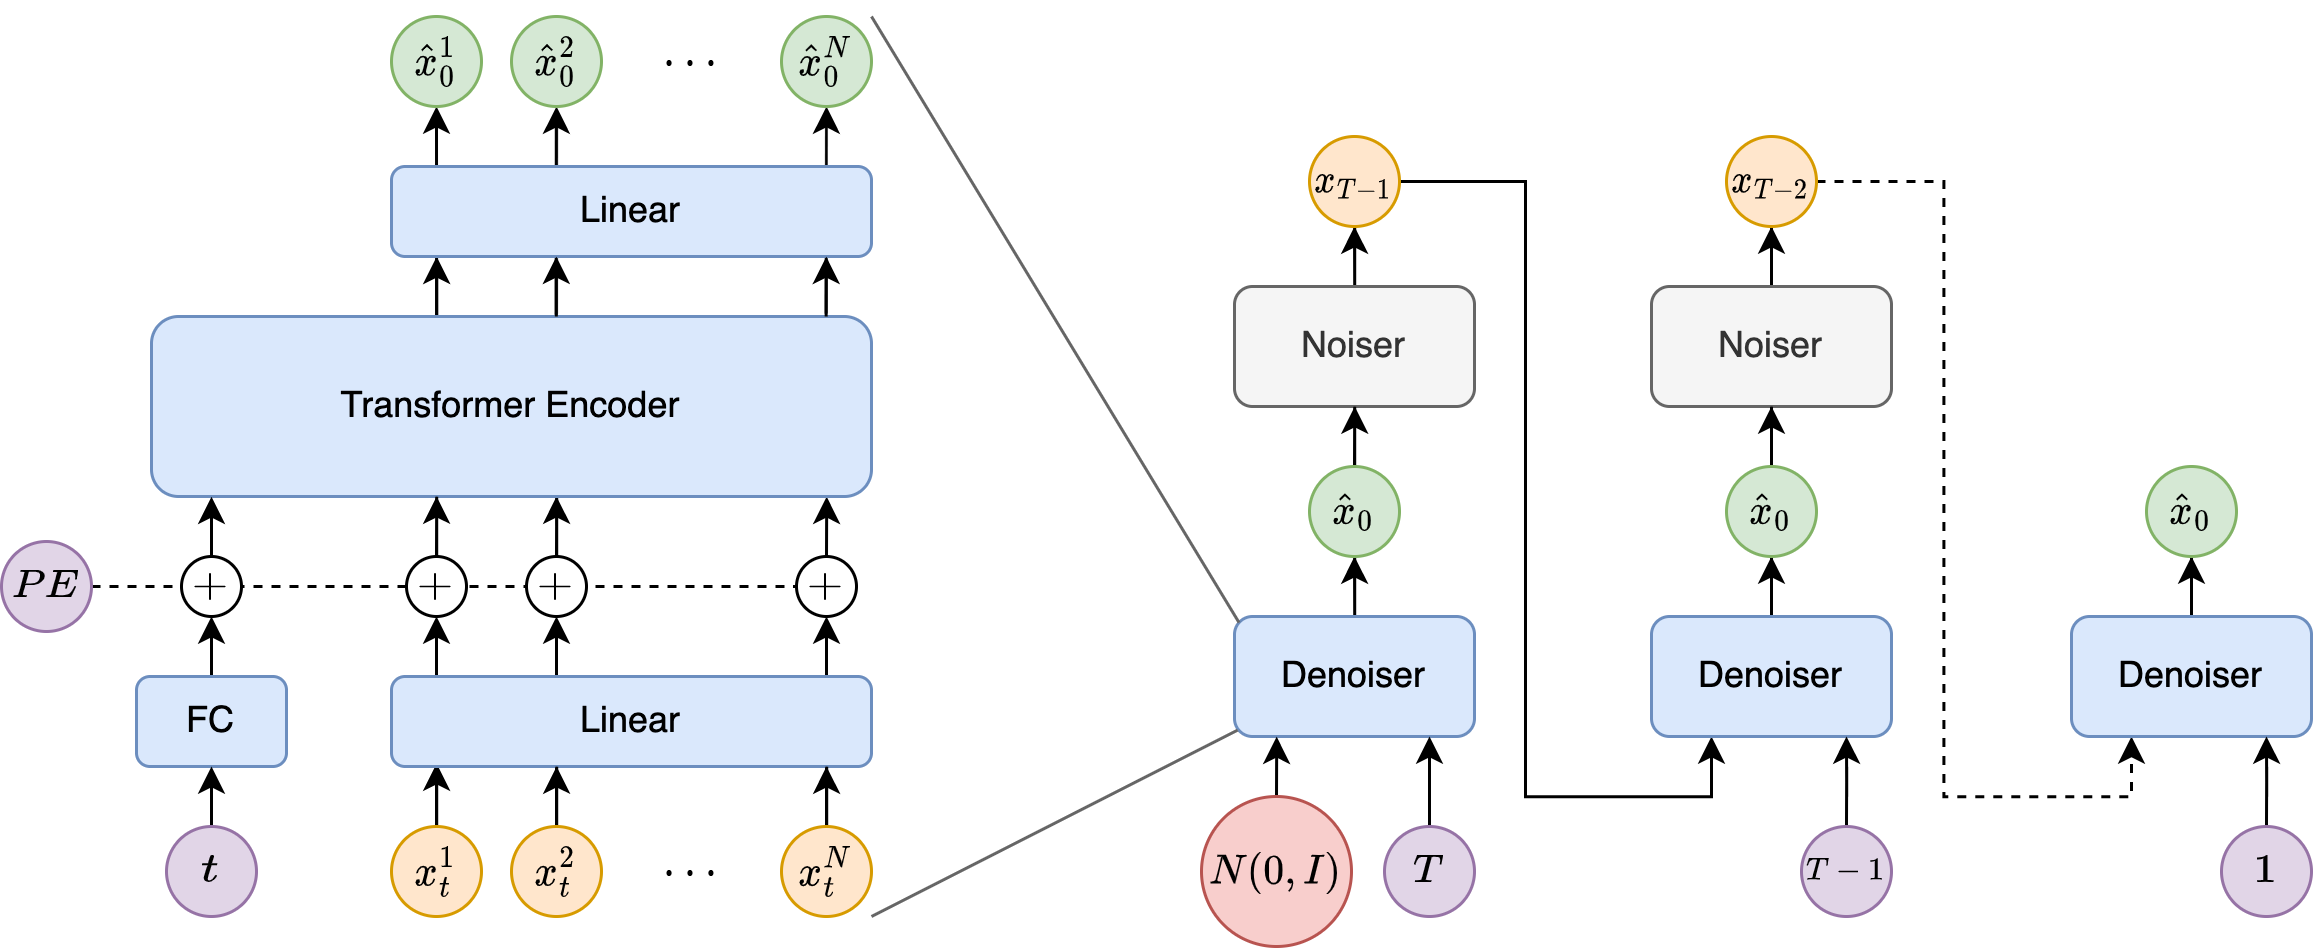
\includegraphics[width=1\textwidth]{Figures/diffusion/Network_diagram.png}
    \caption{Motion Generation - Baseline model}
    \label{fig:baseline_generation}
\end{figure}

\subsubsection{Denoising}
\TODO{Come up with a better test for this}

\subsubsection{Occluded Legs}
The model shows a strong performance on the task of inpainting missing legs in a motion sequence, with the result being of leg motion that is often both smooth and well adhering to the upper body motion. A few examples frames are shown in \figref{fig:baseline_occluded_legs}. 
The most notable failure case is that sometimes the model reverses the direction of motion. We postulate that this is due to the fact that the data for the baseline model has a root that does not move in the forward/reverse direction, therefore the pendulating rotation motion of the hips, without the additional context of a specific direction, can often be both interpreted as both forward and backward motion.

\begin{figure}[!ht]
    \centering
    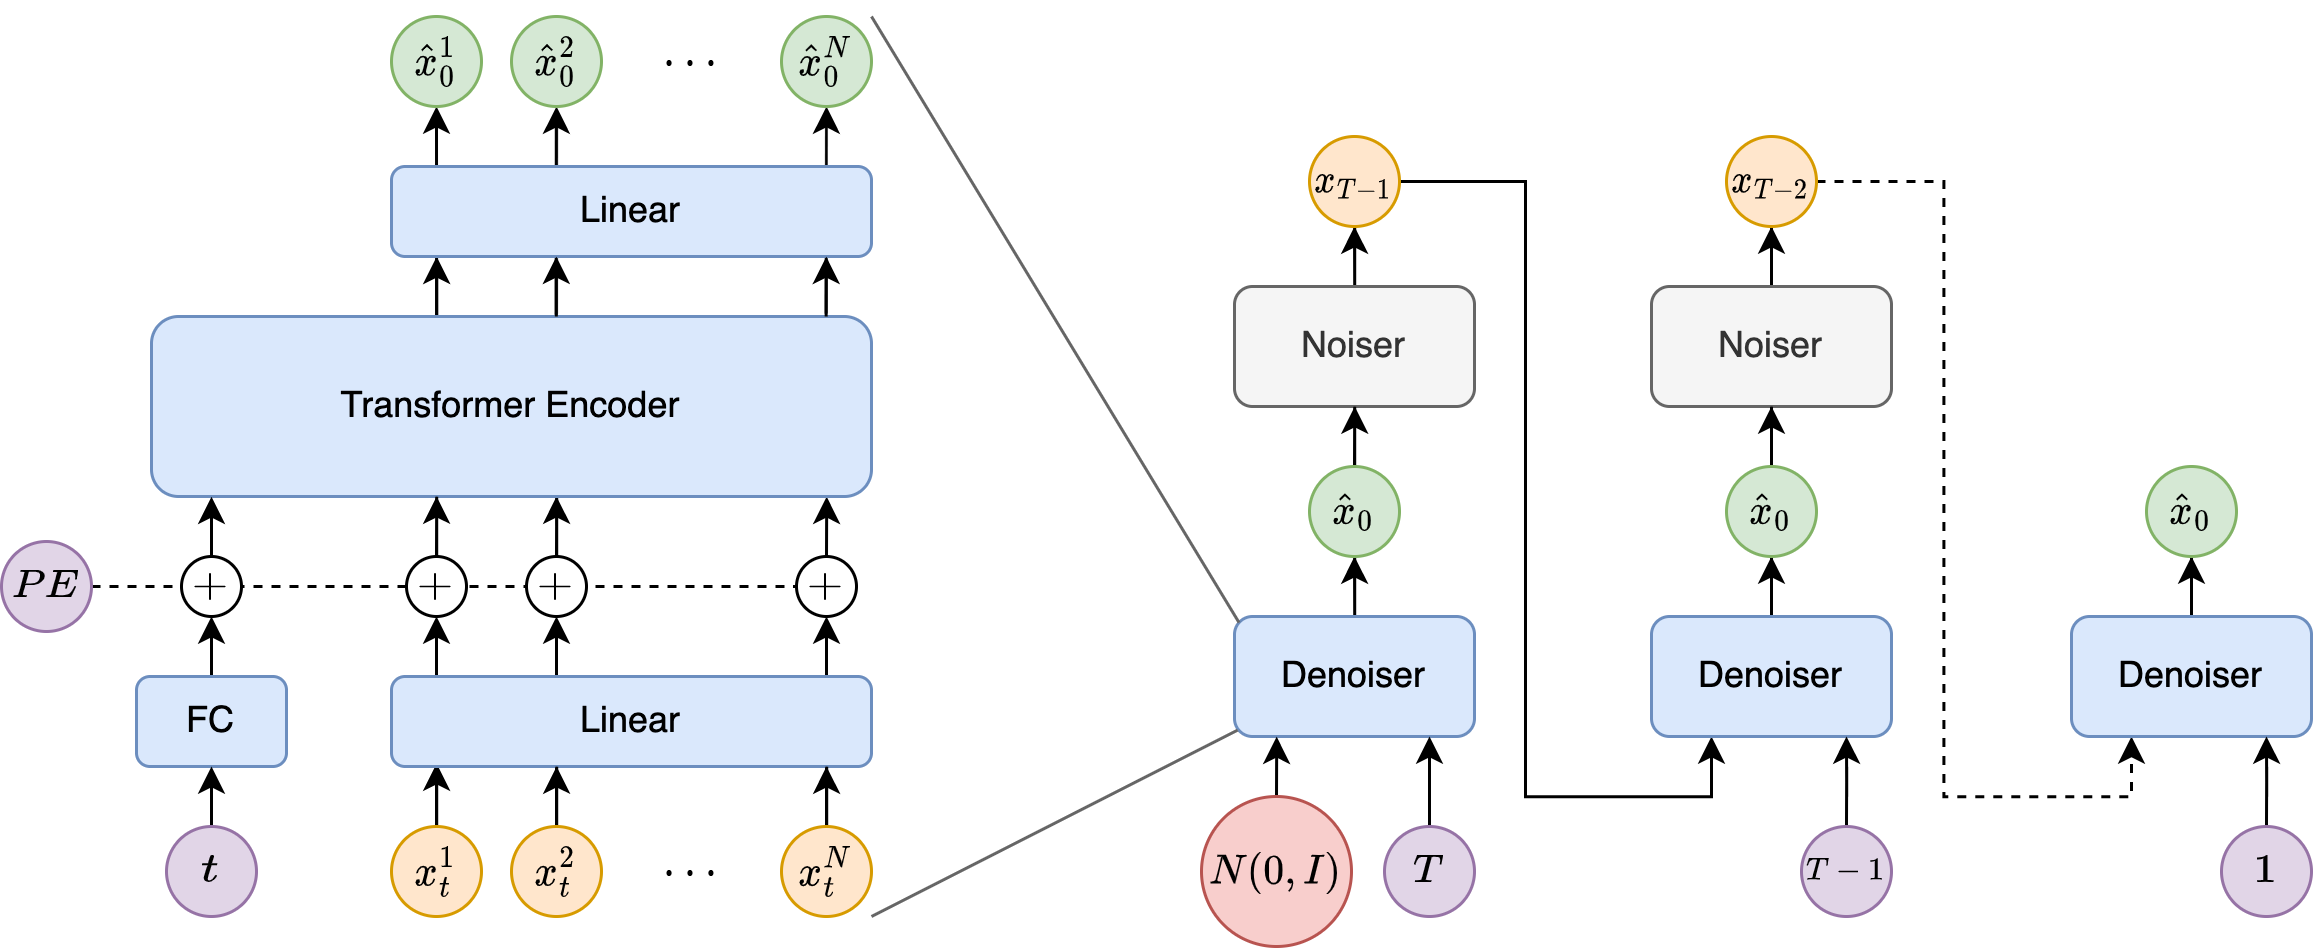
\includegraphics[width=1\textwidth]{Figures/diffusion/Network_diagram.png}
    \caption{Occluded Legs Inpainting - Baseline model}
    \label{fig:baseline_occluded_legs}
\end{figure}


\subsubsection{Missing State}
\textbf{Random each frame}
When removing a new random subset of the joints of each pose every frame in the motion sequence, we find that the model can very accurately reconstruct the missing state, even when only 50\% of the state is given each frame, and surprisingly it still performs reasonably well when only 25\% of the state is given each frame. A few example frames are shown in \figref{fig:baseline_missing_state_random_frame}. This shows that the model has learned well the concept of temporal consistency, as in this experiment it is likely that a missing joint will be surrounded (temporally) by given joints, hence it simply needs to interpolate between the given joints.

\begin{figure}[!ht]
    \centering
    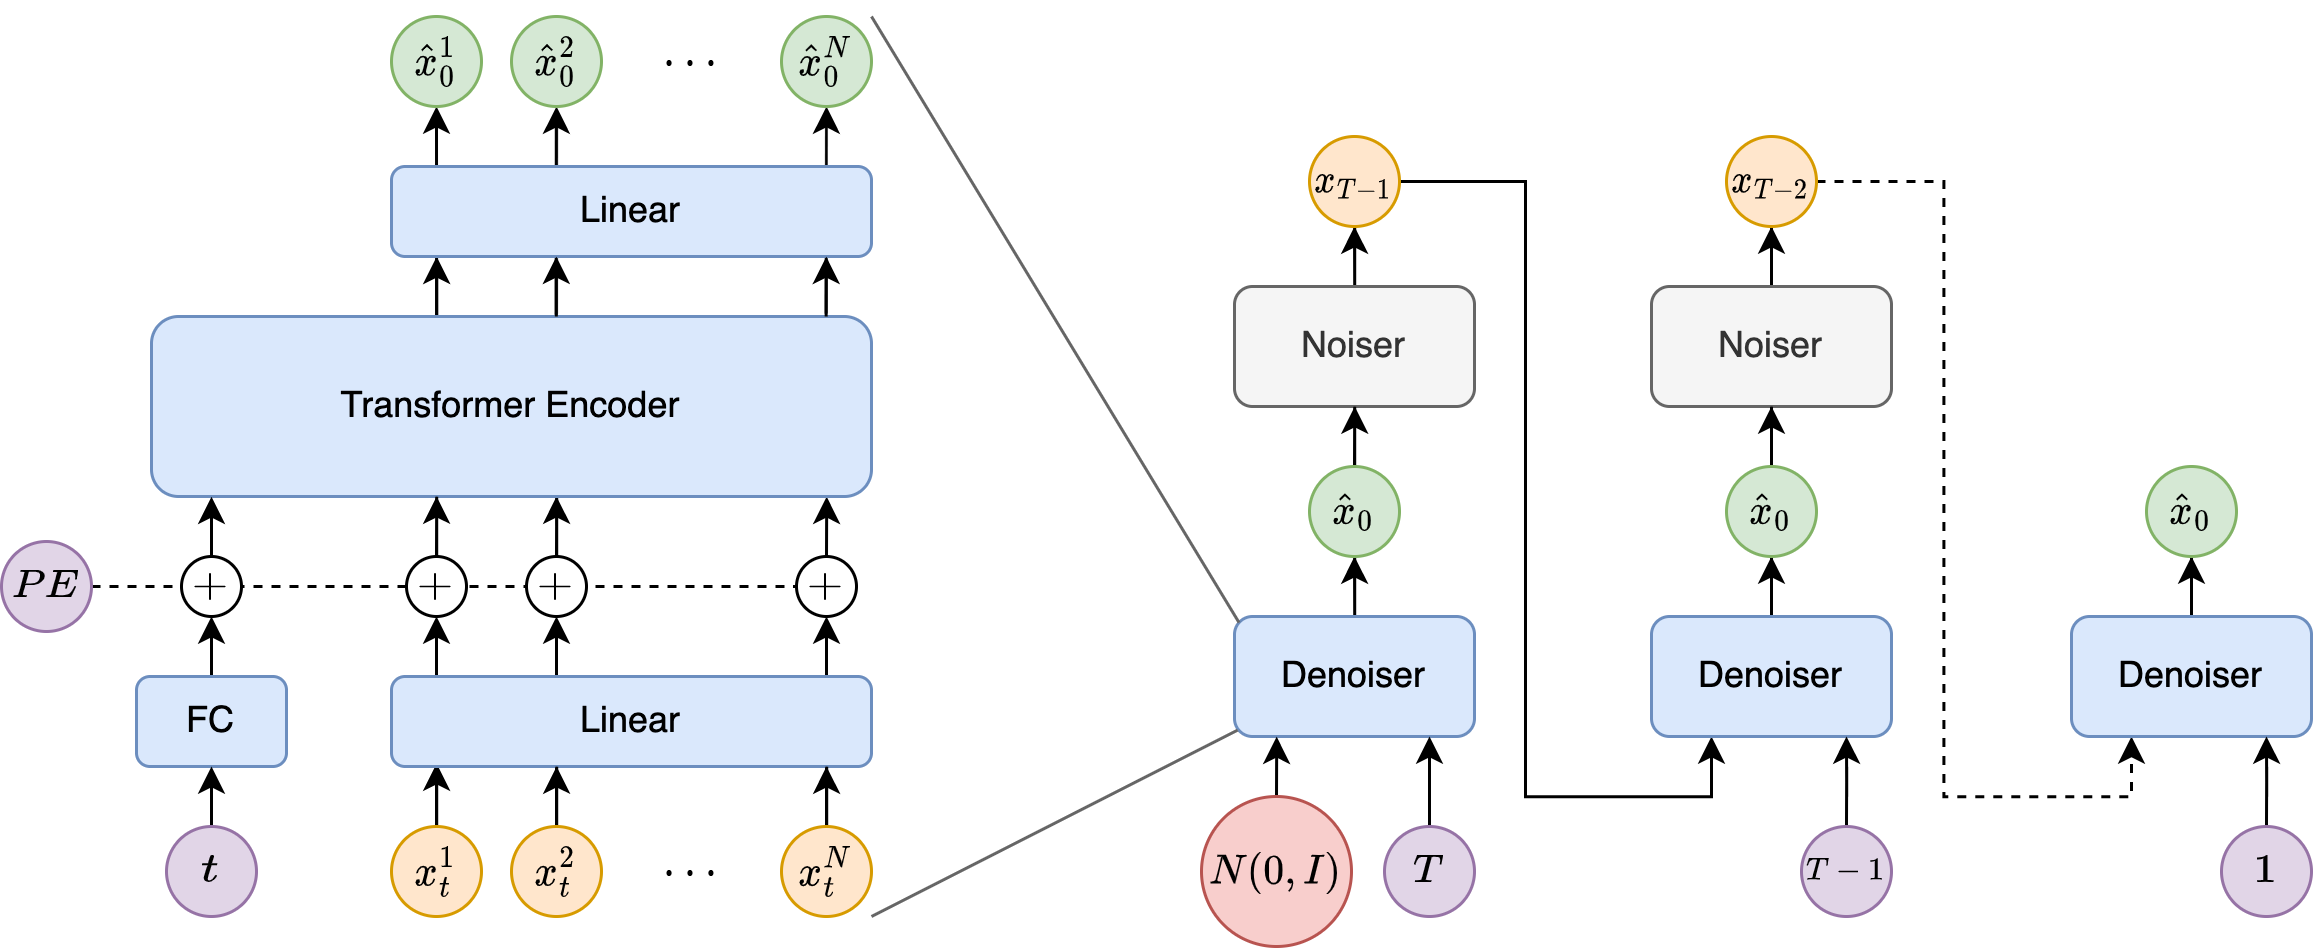
\includegraphics[width=1\textwidth]{Figures/diffusion/Network_diagram.png}
    \caption{Occluded Legs Inpainting - Baseline model}
    \label{fig:baseline_occluded_legs}
\end{figure}

\textbf{Random for the whole sequence}
\TODO{Describe better}


\subsubsection{Inbetweening}


%%%%%%%%%%%%%%%%%%%%%%%%%%%%%%%%%%%%%%%%%%%%%%%%%%%%%%%%%%%%%%%%%%%%%%%%%
% Mode with foot contacts
%%%%%%%%%%%%%%%%%%%%%%%%%%%%%%%%%%%%%%%%%%%%%%%%%%%%%%%%%%%%%%%%%%%%%%%%%
\subsection{Model with Foot Contacts}

\subsubsection{Sequence Generation}
\subsubsection{Denoising}
\subsubsection{Occluded Legs}
\subsubsection{Missing State}
\subsubsection{Inbetweening}


%%%%%%%%%%%%%%%%%%%%%%%%%%%%%%%%%%%%%%%%%%%%%%%%%%%%%%%%%%%%%%%%%%%%%%%%%
% Mode with foot contacts
%%%%%%%%%%%%%%%%%%%%%%%%%%%%%%%%%%%%%%%%%%%%%%%%%%%%%%%%%%%%%%%%%%%%%%%%%
\subsection{Autocompletion}
\label{sec:autocomplete}

Another project that is running at Disney Research|Studios is that of pose autocompletion. This is the task of taking a set of \textit{handles}, a subset of joints, and predicting the position of the rest of the joints. The goal here is to again help to improve the animation pipeline, by reducing the amount of work an animator has to do to get a sensible pose. As a side note to the previous experiments, we train
ed some diffusion models for the described task, where we enforce a sequence length of 1 so that we are only predicting  single pose, and where we modify the inpainting to allow for a specific set of joints to be deemed \textit{handles} and to be kept fixed.

\subsubsection{Baseline}
The model is as described in \secref{sec:baseline_evaluation} however with a sequence length of 1.

We find that while the model does present plausible poses, and that on average these poses have handle joints close to the desired positions of the handles (with a few exceptions), it does not satisfy the task properly as can be seen in \TODO{include images of position of handles vs. position of actual joints}. An ideal solution would not move the handles at all, and would simply modify the rest of the joints.

\TODO{include images}


\subsubsection{Handle Conditioning}
To mitigate this issue of the handles being modified, we propose a handles conditioning, in which a one hot embedding of the handles is run through a linear layer, then concatenated to the input of the network. A loss is then applied to the output that penalises any deviation in position of the handles that are output as compared to those input. In theory this should force the network to learn to consider the handles as immutable, and to create a pose that satisfies the handles.

Though the implementation was largely completed, we unfortunately did not have time to finish debugging some of the finer details, and so cannot provide concrete results. However we deemed the idea interesting enough to present in this thesis, and hope that it can be of use in future research directions.
\section{Conclusion}
\chapter{Conclusion and Outlook}
\label{chpt:conclusion}

We embarked upon the work presented in this thesis to explore motion modeling in the context of a project at Disney Research|Studios aiming to capture motion data direct from RGB videos. To begin with, we explored the relevant literature in \chpref{chpt:related_work}, gaining a broader understanding of the field of motion modeling, and placing emphasis on the common Autoencoder and VAE architectures and the promising field of diffusion models. Next, we selected the HuMoR method \cite{humor} as a base for an investigation, with the view that the model's strong performance and use for rectifying motion sequences obtained from 2d pose estimates could lead to an important improvement of the existing Disney Research|Studious pipeline. We investigated the model in \chpref{chpt:humor}, finding that the model provided promising result however at a huge computational cost. We set out to improve this speed issue in \secref{sec:humor_improvement}, presenting a novel strategy for optimisation that broke the autoregressive nature of the HuMoR method at the heart of the performance issue. Considerable effort was made to obtain comparable results, however the conclusion was reached that the results were not nearing the required quality and that the desired speedup seemed tricky to achieve. With the lessons of this experience on hand we formulated a new research direction, choosing to investigate a sequence-level model, rather than the local pose-to-pose model of HuMoR due to the large potential speedup, and moved to the novel diffusion framework for which a promising literature is emerging. We explored in detail the diffusion framework in \chpref{chpt:diffusion} and formulated a baseline architecture upon which to base our investigations. We evaluated on a wide range of different tasks in \secref{sec:diffusion_experiments}, finding that the model can successfully replace missing legs and random missing joints, that it shows promise for motion inbetweening, that it generates diverse plausible motion, that it can be used for other tasks such as pose autocompletion, that the diffusion denoising procedure is flexible and can be sped up, and that the inpainting procedure can be modified to improve performance. Finally, we discussed the many exciting future research directions in \secref{sec:diffusion_future_work}. We are hopeful for the future of diffusion models in motion modeling and are thrilled to have provided a notion of their potential and a building block upon which to base future research.

% ---- END MAIN PART ----


\appendix
\clearpage
\renewcommand*{\chapterpagestyle}{myappendixpagestyle}

\chapter{Information For The Few}

Nein, meine Texte les ich nicht, so nicht, st?hnte Oxmox. Er war mit Franklin, Rockwell und dem halbtaxgrauen Panther Weidemann in Memphis (Heartbreak Hotel) zugange. Sie warteten auf die fette Gill, um bei der Bank of Helvetica die Kapit?lchen in Kapital umzuwandeln. Oxmox liess nicht locker. Ich fleh euch an, rettet meine Copy, gebt meinem Body nochn Durchschuss! Kein Problem, erbarmte sich Old Face Baskerville, streichelte seinen Hund, zog seine einspaltige Poppl, legte an und traf! (Zeidank nichts Ernstes --- nurn bisschen Fraktur.) Oxmox: Danke, ist jetzt mit Abstand besser. Derweil jumpte der Fox leise over the Buhl, die sich mal wieder immerdar wie jedes Jahr gesellte. Diesmal war Guaredisch ihr Erw?hlter, weil seine Laufweite einem vollgetankten Bodoni entsprach und seine ungez?gelte Unterl?nge ihre Serifen so serafisch streifte, dass sie trotz Techtelmechtelei die magere Futura, jene zuverl?ssige und gern eingesetzte Langstreckenl?uferin, rechtsb?ndig ?berholen konnten.

\section{Foo Bar Baz}

Nein, meine Texte les ich nicht, so nicht, st?hnte Oxmox. Er war mit Franklin, Rockwell und dem halbtaxgrauen Panther Weidemann in Memphis (Heartbreak Hotel) zugange. Sie warteten auf die fette Gill, um bei der Bank of Helvetica die Kapit?lchen in Kapital umzuwandeln. Oxmox liess nicht locker. Ich fleh euch an, rettet meine Copy, gebt meinem Body nochn Durchschuss! Kein Problem, erbarmte sich Old Face Baskerville, streichelte seinen Hund, zog seine einspaltige Poppl, legte an und traf! (Zeidank nichts Ernstes --- nurn bisschen Fraktur.) Oxmox: Danke, ist jetzt mit Abstand besser. Derweil jumpte der Fox leise over the Buhl, die sich mal wieder immerdar wie jedes Jahr gesellte. Diesmal war Guaredisch ihr Erw?hlter, weil seine Laufweite einem vollgetankten Bodoni entsprach und seine ungez?gelte Unterl?nge ihre Serifen so serafisch streifte, dass sie trotz Techtelmechtelei die magere Futura, jene zuverl?ssige und gern eingesetzte Langstreckenl?uferin, rechtsb?ndig ?berholen konnten.

\section{Barontes}

Nein, meine Texte les ich nicht, so nicht, st?hnte Oxmox. Er war mit Franklin, Rockwell und dem halbtaxgrauen Panther Weidemann in Memphis (Heartbreak Hotel) zugange. Sie warteten auf die fette Gill, um bei der Bank of Helvetica die Kapit?lchen in Kapital umzuwandeln. Oxmox liess nicht locker. Ich fleh euch an, rettet meine Copy, gebt meinem Body nochn Durchschuss! Kein Problem, erbarmte sich Old Face Baskerville, streichelte seinen Hund, zog seine einspaltige Poppl, legte an und traf! (Zeidank nichts Ernstes --- nurn bisschen Fraktur.) Oxmox: Danke, ist jetzt mit Abstand besser. Derweil jumpte der Fox leise over the Buhl, die sich mal wieder immerdar wie jedes Jahr gesellte. Diesmal war Guaredisch ihr Erw?hlter, weil seine Laufweite einem vollgetankten Bodoni entsprach und seine ungez?gelte Unterl?nge ihre Serifen so serafisch streifte, dass sie trotz Techtelmechtelei die magere Futura, jene zuverl?ssige und gern eingesetzte Langstreckenl?uferin, rechtsb?ndig ?berholen konnten.


\section{A Long Table with Booktabs}


{\scriptsize
\begin{longtable}{clccccccc}
\caption[wordlist]{A sample list of words.}\\
\toprule
ID & Word & Word Length & WD & ETL & PTL &  WDplus \\
\midrule
\endfirsthead
\caption[]{(Continued)}\\
\toprule
ID & Word & Word Length & WD & ETL & PTL &  WDplus \\
\midrule
\endhead
\midrule
\multicolumn{9}{c}{continued on next page}\\
\bottomrule
\endfoot
%\bottomrule
\endlastfoot
\hline
1 & Eis & 3 & 4 & 0.42 & 1.83 & 0.19 \\ \hline
2 & Mai & 3 & 5 & 0.49 & 1.92 & 0.19 \\ \hline
3 & Art & 3 & 5 & 0.27 & 1.67 & 0.14 \\ \hline
4 & Uhr & 3 & 5 & 0.57 & 1.87 & 0.36 \\ \hline
5 & Rat & 3 & 5 & 0.36 & 1.71 & 0.14 \\ \hline
6 & weit & 4 & 6 & 0.21 & 1.65 & 0.25 \\ \hline
7 & eins & 4 & 6 & 0.38 & 1.79 & 0.26 \\ \hline
8 & Wort & 4 & 6 & 0.30 & 1.62 & 0.20 \\ \hline
9 & Wolf & 4 & 6 & 0.18 & 1.54 & 0.19 \\ \hline
10 & Wald & 4 & 6 & 0.31 & 1.63 & 0.19 \\ \hline
11 & Amt & 3 & 6 & 0.30 & 1.67 & 0.14 \\ \hline
12 & Wahl & 4 & 7 & 0.36 & 1.77 & 0.42 \\ \hline
13 & Volk & 4 & 7 & 0.45 & 1.81 & 0.20 \\ \hline
14 & Ziel & 4 & 7 & 0.48 & 1.78 & 0.42 \\ \hline
15 & vier & 4 & 7 & 0.38 & 1.81 & 0.42 \\ \hline
16 & Kreis & 5 & 7 & 0.26 & 1.62 & 0.33 \\ \hline
17 & Preis & 5 & 7 & 0.28 & 1.51 & 0.33 \\ \hline
18 & Re-de & 4 & 7 & 0.22 & 1.56 & 0.33 \\ \hline
19 & Saal & 4 & 7 & 0.75 & 2.10 & 0.43 \\ \hline
20 & voll & 4 & 7 & 0.48 & 1.82 & 0.24 \\ \hline
21 & weiss & 5 & 7 & 0.21 & 1.59 & 0.36 \\ \hline
22 & ?r-ger & 5 & 7 & 1.16 & 2.69 & 0.59 \\ \hline
23 & bald & 4 & 7 & 0.18 & 1.56 & 0.19 \\ \hline
24 & hier & 4 & 7 & 0.40 & 1.70 & 0.43 \\ \hline
25 & neun & 4 & 7 & 0.17 & 1.52 & 0.26 \\ \hline
26 & sehr & 4 & 7 & 0.36 & 1.85 & 0.43 \\ \hline
27 & Jahr & 4 & 7 & 0.50 & 1.82 & 0.43 \\ \hline
28 & Gold & 4 & 7 & 0.04 & 1.35 & 0.20 \\ \hline
29 & T?-ter & 5 & 8 & 0.15 & 1.39 & 0.59 \\ \hline
30 & Tei-le & 5 & 8 & 0.30 & 1.71 & 0.46 \\ \hline
31 & Na-tur & 5 & 8 & 0.18 & 1.59 & 0.41 \\ \hline
32 & Feu-er & 5 & 8 & 0.30 & 1.71 & 0.45 \\ \hline
33 & Rol-le & 5 & 8 & 0.15 & 1.46 & 0.45 \\ \hline
34 & Rock & 4 & 8 & 0.29 & 1.68 & 0.25 \\ \hline
35 & Spass & 5 & 8 & 0.28 & 1.64 & 0.32 \\ \hline
36 & G?s-te & 5 & 8 & 0.49 & 1.75 & 0.66 \\ \hline
37 & En-de & 4 & 8 & 0.36 & 1.72 & 0.33 \\ \hline
38 & Kunst & 5 & 8 & 0.26 & 1.59 & 0.35 \\ \hline
39 & Li-nie & 5 & 8 & 0.45 & 1.88 & 0.63 \\ \hline
40 & B?u-me & 5 & 8 & 0.48 & 1.92 & 0.45 \\ \hline
41 & B?h-ne & 5 & 9 & 0.94 & 2.48 & 0.62 \\ \hline
42 & Bahn & 4 & 9 & 0.21 & 1.62 & 0.42 \\ \hline
43 & B?r-ger & 6 & 9 & 0.38 & 1.70 & 0.65 \\ \hline
44 & Druck & 5 & 9 & 0.60 & 2.03 & 0.31 \\ \hline
45 & zehn & 4 & 9 & 0.41 & 1.84 & 0.42 \\ \hline
46 & Va-ter & 5 & 9 & 0.36 & 1.78 & 0.40 \\ \hline
47 & Angst & 5 & 9 & 0.29 & 1.56 & 0.35 \\ \hline
48 & lei-der & 6 & 9 & 0.13 & 1.47 & 0.52 \\ \hline
49 & h?u-fig & 6 & 9 & 0.82 & 2.31 & 0.52 \\ \hline
50 & le-ben & 5 & 9 & 0.38 & 1.85 & 0.40 \\ \hline
51 & aus-ser & 6 & 9 & 1.20 & 2.26 & 0.57 \\ \hline
52 & be-vor & 5 & 9 & 1.28 & 2.75 & 0.39 \\ \hline
53 & Kai-ser & 6 & 9 & 0.92 & 2.37 & 0.53 \\ \hline
54 & Markt & 5 & 9 & 0.23 & 1.58 & 0.28 \\ \hline
55 & Os-ten & 5 & 9 & 0.21 & 1.54 & 0.48 \\ \hline
56 & Krieg & 5 & 9 & 0.33 & 1.67 & 0.50 \\ \hline
57 & Mann & 4 & 9 & 0.31 & 1.47 & 0.25 \\ \hline
58 & Hal-le & 5 & 9 & 0.24 & 1.65 & 0.45 \\ \hline
59 & heu-te & 5 & 9 & 0.44 & 1.87 & 0.46 \\ \hline
60 & in-nen & 5 & 10 & 0.36 & 1.80 & 0.45 \\ \hline
61 & Na-men & 5 & 10 & 0.28 & 1.72 & 0.41 \\ \hline
62 & jetzt & 5 & 10 & 0.70 & 2.07 & 0.32 \\ \hline
63 & kei-ner & 6 & 10 & 0.28 & 1.62 & 0.53 \\ \hline
64 & Schu-le & 6 & 10 & 1.02 & 2.12 & 0.48 \\ \hline
65 & Ar-beit & 6 & 10 & 0.34 & 1.70 & 0.52 \\ \hline
66 & An-teil & 6 & 10 & 0.27 & 1.63 & 0.53 \\ \hline
67 & di-rekt & 6 & 10 & 0.67 & 2.04 & 0.47 \\ \hline
68 & vor-her & 6 & 10 & 0.78 & 2.25 & 0.47 \\ \hline
69 & wol-len & 6 & 10 & 0.44 & 1.85 & 0.51 \\ \hline
70 & Kampf & 5 & 10 & 0.70 & 1.96 & 0.27 \\ \hline
71 & ?n-dern & 6 & 10 & 1.18 & 2.62 & 0.65 \\ \hline
72 & lau-fen & 6 & 10 & 0.21 & 1.64 & 0.52 \\ \hline
73 & Eu-ro-pa & 6 & 10 & 0.23 & 1.53 & 0.66 \\ \hline
74 & statt & 5 & 10 & 1.61 & 2.86 & 0.39 \\ \hline
75 & Wes-ten & 6 & 10 & 0.29 & 1.60 & 0.54 \\
\bottomrule
\label{tab:wordlist}
\end{longtable}
}

\clearpage
\renewcommand*{\chapterpagestyle}{empty}

%\nocite{*}
\addcontentsline{toc}{chapter}{Bibliography}
\bibliography{bibliography}

\end{document}
